\documentclass[11pt]{article}

    \usepackage[breakable]{tcolorbox}
    \usepackage{parskip} % Stop auto-indenting (to mimic markdown behaviour)
    

    % Basic figure setup, for now with no caption control since it's done
    % automatically by Pandoc (which extracts ![](path) syntax from Markdown).
    \usepackage{graphicx}
    \usepackage{ctex}
    % Keep aspect ratio if custom image width or height is specified
    \setkeys{Gin}{keepaspectratio}
    % Maintain compatibility with old templates. Remove in nbconvert 6.0
    \let\Oldincludegraphics\includegraphics
    % Ensure that by default, figures have no caption (until we provide a
    % proper Figure object with a Caption API and a way to capture that
    % in the conversion process - todo).
    \usepackage{caption}
    \usepackage{endnotes}
    \usepackage{hyperref}
    \usepackage[backend=biber,style=ieee]{biblatex}
    \addbibresource{references.bib}
    \DeclareCaptionFormat{nocaption}{}
    \captionsetup{format=nocaption,aboveskip=0pt,belowskip=0pt}

    \usepackage{float}
    \floatplacement{figure}{H} % forces figures to be placed at the correct location
    \usepackage{xcolor} % Allow colors to be defined
    \usepackage{enumerate} % Needed for markdown enumerations to work
    \usepackage{geometry} % Used to adjust the document margins
    \usepackage{amsmath} % Equations
    \usepackage{amssymb} % Equations
    \usepackage{textcomp} % defines textquotesingle
    % Hack from http://tex.stackexchange.com/a/47451/13684:
    \AtBeginDocument{%
        \def\PYZsq{\textquotesingle}% Upright quotes in Pygmentized code
    }
    \usepackage{upquote} % Upright quotes for verbatim code
    \usepackage{eurosym} % defines \euro

    \usepackage{iftex}
    \ifPDFTeX
        \usepackage[T1]{fontenc}
        \IfFileExists{alphabeta.sty}{
              \usepackage{alphabeta}
          }{
              \usepackage[mathletters]{ucs}
              \usepackage[utf8x]{inputenc}
          }
    \else
        \usepackage{fontspec}
        \usepackage{unicode-math}
    \fi

    \usepackage{fancyvrb} % verbatim replacement that allows latex
    \usepackage{grffile} % extends the file name processing of package graphics
                         % to support a larger range
    \makeatletter % fix for old versions of grffile with XeLaTeX
    \@ifpackagelater{grffile}{2019/11/01}
    {
      % Do nothing on new versions
    }
    {
      \def\Gread@@xetex#1{%
        \IfFileExists{"\Gin@base".bb}%
        {\Gread@eps{\Gin@base.bb}}%
        {\Gread@@xetex@aux#1}%
      }
    }
    \makeatother
    \usepackage[Export]{adjustbox} % Used to constrain images to a maximum size
    \adjustboxset{max size={0.9\linewidth}{0.9\paperheight}}

    % The hyperref package gives us a pdf with properly built
    % internal navigation ('pdf bookmarks' for the table of contents,
    % internal cross-reference links, web links for URLs, etc.)
    \usepackage{hyperref}
    % The default LaTeX title has an obnoxious amount of whitespace. By default,
    % titling removes some of it. It also provides customization options.
    \usepackage{titling}
    \usepackage{longtable} % longtable support required by pandoc >1.10
    \usepackage{booktabs}  % table support for pandoc > 1.12.2
    \usepackage{array}     % table support for pandoc >= 2.11.3
    \usepackage{calc}      % table minipage width calculation for pandoc >= 2.11.1
    \usepackage[inline]{enumitem} % IRkernel/repr support (it uses the enumerate* environment)
    \usepackage[normalem]{ulem} % ulem is needed to support strikethroughs (\sout)
                                % normalem makes italics be italics, not underlines
    \usepackage{soul}      % strikethrough (\st) support for pandoc >= 3.0.0
    \usepackage{mathrsfs}
    

    
    % Colors for the hyperref package
    \definecolor{urlcolor}{rgb}{0,.145,.698}
    \definecolor{linkcolor}{rgb}{.71,0.21,0.01}
    \definecolor{citecolor}{rgb}{.12,.54,.11}

    % ANSI colors
    \definecolor{ansi-black}{HTML}{3E424D}
    \definecolor{ansi-black-intense}{HTML}{282C36}
    \definecolor{ansi-red}{HTML}{E75C58}
    \definecolor{ansi-red-intense}{HTML}{B22B31}
    \definecolor{ansi-green}{HTML}{00A250}
    \definecolor{ansi-green-intense}{HTML}{007427}
    \definecolor{ansi-yellow}{HTML}{DDB62B}
    \definecolor{ansi-yellow-intense}{HTML}{B27D12}
    \definecolor{ansi-blue}{HTML}{208FFB}
    \definecolor{ansi-blue-intense}{HTML}{0065CA}
    \definecolor{ansi-magenta}{HTML}{D160C4}
    \definecolor{ansi-magenta-intense}{HTML}{A03196}
    \definecolor{ansi-cyan}{HTML}{60C6C8}
    \definecolor{ansi-cyan-intense}{HTML}{258F8F}
    \definecolor{ansi-white}{HTML}{C5C1B4}
    \definecolor{ansi-white-intense}{HTML}{A1A6B2}
    \definecolor{ansi-default-inverse-fg}{HTML}{FFFFFF}
    \definecolor{ansi-default-inverse-bg}{HTML}{000000}

    % common color for the border for error outputs.
    \definecolor{outerrorbackground}{HTML}{FFDFDF}

    % commands and environments needed by pandoc snippets
    % extracted from the output of `pandoc -s`
    \providecommand{\tightlist}{%
      \setlength{\itemsep}{0pt}\setlength{\parskip}{0pt}}
    \DefineVerbatimEnvironment{Highlighting}{Verbatim}{commandchars=\\\{\}}
    % Add ',fontsize=\small' for more characters per line
    \newenvironment{Shaded}{}{}
    \newcommand{\KeywordTok}[1]{\textcolor[rgb]{0.00,0.44,0.13}{\textbf{{#1}}}}
    \newcommand{\DataTypeTok}[1]{\textcolor[rgb]{0.56,0.13,0.00}{{#1}}}
    \newcommand{\DecValTok}[1]{\textcolor[rgb]{0.25,0.63,0.44}{{#1}}}
    \newcommand{\BaseNTok}[1]{\textcolor[rgb]{0.25,0.63,0.44}{{#1}}}
    \newcommand{\FloatTok}[1]{\textcolor[rgb]{0.25,0.63,0.44}{{#1}}}
    \newcommand{\CharTok}[1]{\textcolor[rgb]{0.25,0.44,0.63}{{#1}}}
    \newcommand{\StringTok}[1]{\textcolor[rgb]{0.25,0.44,0.63}{{#1}}}
    \newcommand{\CommentTok}[1]{\textcolor[rgb]{0.38,0.63,0.69}{\textit{{#1}}}}
    \newcommand{\OtherTok}[1]{\textcolor[rgb]{0.00,0.44,0.13}{{#1}}}
    \newcommand{\AlertTok}[1]{\textcolor[rgb]{1.00,0.00,0.00}{\textbf{{#1}}}}
    \newcommand{\FunctionTok}[1]{\textcolor[rgb]{0.02,0.16,0.49}{{#1}}}
    \newcommand{\RegionMarkerTok}[1]{{#1}}
    \newcommand{\ErrorTok}[1]{\textcolor[rgb]{1.00,0.00,0.00}{\textbf{{#1}}}}
    \newcommand{\NormalTok}[1]{{#1}}

    % Additional commands for more recent versions of Pandoc
    \newcommand{\ConstantTok}[1]{\textcolor[rgb]{0.53,0.00,0.00}{{#1}}}
    \newcommand{\SpecialCharTok}[1]{\textcolor[rgb]{0.25,0.44,0.63}{{#1}}}
    \newcommand{\VerbatimStringTok}[1]{\textcolor[rgb]{0.25,0.44,0.63}{{#1}}}
    \newcommand{\SpecialStringTok}[1]{\textcolor[rgb]{0.73,0.40,0.53}{{#1}}}
    \newcommand{\ImportTok}[1]{{#1}}
    \newcommand{\DocumentationTok}[1]{\textcolor[rgb]{0.73,0.13,0.13}{\textit{{#1}}}}
    \newcommand{\AnnotationTok}[1]{\textcolor[rgb]{0.38,0.63,0.69}{\textbf{\textit{{#1}}}}}
    \newcommand{\CommentVarTok}[1]{\textcolor[rgb]{0.38,0.63,0.69}{\textbf{\textit{{#1}}}}}
    \newcommand{\VariableTok}[1]{\textcolor[rgb]{0.10,0.09,0.49}{{#1}}}
    \newcommand{\ControlFlowTok}[1]{\textcolor[rgb]{0.00,0.44,0.13}{\textbf{{#1}}}}
    \newcommand{\OperatorTok}[1]{\textcolor[rgb]{0.40,0.40,0.40}{{#1}}}
    \newcommand{\BuiltInTok}[1]{{#1}}
    \newcommand{\ExtensionTok}[1]{{#1}}
    \newcommand{\PreprocessorTok}[1]{\textcolor[rgb]{0.74,0.48,0.00}{{#1}}}
    \newcommand{\AttributeTok}[1]{\textcolor[rgb]{0.49,0.56,0.16}{{#1}}}
    \newcommand{\InformationTok}[1]{\textcolor[rgb]{0.38,0.63,0.69}{\textbf{\textit{{#1}}}}}
    \newcommand{\WarningTok}[1]{\textcolor[rgb]{0.38,0.63,0.69}{\textbf{\textit{{#1}}}}}


    % Define a nice break command that doesn't care if a line doesn't already
    % exist.
    \def\br{\hspace*{\fill} \\* }
    % Math Jax compatibility definitions
    \def\gt{>}
    \def\lt{<}
    \let\Oldtex\TeX
    \let\Oldlatex\LaTeX
    \renewcommand{\TeX}{\textrm{\Oldtex}}
    \renewcommand{\LaTeX}{\textrm{\Oldlatex}}
    % Document parameters
    % Document title
    \title{Report on Reverse Engineering the Mechanism of \\ Wechat Red Envelop}
    
% Pygments definitions
\makeatletter
\def\PY@reset{\let\PY@it=\relax \let\PY@bf=\relax%
    \let\PY@ul=\relax \let\PY@tc=\relax%
    \let\PY@bc=\relax \let\PY@ff=\relax}
\def\PY@tok#1{\csname PY@tok@#1\endcsname}
\def\PY@toks#1+{\ifx\relax#1\empty\else%
    \PY@tok{#1}\expandafter\PY@toks\fi}
\def\PY@do#1{\PY@bc{\PY@tc{\PY@ul{%
    \PY@it{\PY@bf{\PY@ff{#1}}}}}}}
\def\PY#1#2{\PY@reset\PY@toks#1+\relax+\PY@do{#2}}

\@namedef{PY@tok@w}{\def\PY@tc##1{\textcolor[rgb]{0.73,0.73,0.73}{##1}}}
\@namedef{PY@tok@c}{\let\PY@it=\textit\def\PY@tc##1{\textcolor[rgb]{0.24,0.48,0.48}{##1}}}
\@namedef{PY@tok@cp}{\def\PY@tc##1{\textcolor[rgb]{0.61,0.40,0.00}{##1}}}
\@namedef{PY@tok@k}{\let\PY@bf=\textbf\def\PY@tc##1{\textcolor[rgb]{0.00,0.50,0.00}{##1}}}
\@namedef{PY@tok@kp}{\def\PY@tc##1{\textcolor[rgb]{0.00,0.50,0.00}{##1}}}
\@namedef{PY@tok@kt}{\def\PY@tc##1{\textcolor[rgb]{0.69,0.00,0.25}{##1}}}
\@namedef{PY@tok@o}{\def\PY@tc##1{\textcolor[rgb]{0.40,0.40,0.40}{##1}}}
\@namedef{PY@tok@ow}{\let\PY@bf=\textbf\def\PY@tc##1{\textcolor[rgb]{0.67,0.13,1.00}{##1}}}
\@namedef{PY@tok@nb}{\def\PY@tc##1{\textcolor[rgb]{0.00,0.50,0.00}{##1}}}
\@namedef{PY@tok@nf}{\def\PY@tc##1{\textcolor[rgb]{0.00,0.00,1.00}{##1}}}
\@namedef{PY@tok@nc}{\let\PY@bf=\textbf\def\PY@tc##1{\textcolor[rgb]{0.00,0.00,1.00}{##1}}}
\@namedef{PY@tok@nn}{\let\PY@bf=\textbf\def\PY@tc##1{\textcolor[rgb]{0.00,0.00,1.00}{##1}}}
\@namedef{PY@tok@ne}{\let\PY@bf=\textbf\def\PY@tc##1{\textcolor[rgb]{0.80,0.25,0.22}{##1}}}
\@namedef{PY@tok@nv}{\def\PY@tc##1{\textcolor[rgb]{0.10,0.09,0.49}{##1}}}
\@namedef{PY@tok@no}{\def\PY@tc##1{\textcolor[rgb]{0.53,0.00,0.00}{##1}}}
\@namedef{PY@tok@nl}{\def\PY@tc##1{\textcolor[rgb]{0.46,0.46,0.00}{##1}}}
\@namedef{PY@tok@ni}{\let\PY@bf=\textbf\def\PY@tc##1{\textcolor[rgb]{0.44,0.44,0.44}{##1}}}
\@namedef{PY@tok@na}{\def\PY@tc##1{\textcolor[rgb]{0.41,0.47,0.13}{##1}}}
\@namedef{PY@tok@nt}{\let\PY@bf=\textbf\def\PY@tc##1{\textcolor[rgb]{0.00,0.50,0.00}{##1}}}
\@namedef{PY@tok@nd}{\def\PY@tc##1{\textcolor[rgb]{0.67,0.13,1.00}{##1}}}
\@namedef{PY@tok@s}{\def\PY@tc##1{\textcolor[rgb]{0.73,0.13,0.13}{##1}}}
\@namedef{PY@tok@sd}{\let\PY@it=\textit\def\PY@tc##1{\textcolor[rgb]{0.73,0.13,0.13}{##1}}}
\@namedef{PY@tok@si}{\let\PY@bf=\textbf\def\PY@tc##1{\textcolor[rgb]{0.64,0.35,0.47}{##1}}}
\@namedef{PY@tok@se}{\let\PY@bf=\textbf\def\PY@tc##1{\textcolor[rgb]{0.67,0.36,0.12}{##1}}}
\@namedef{PY@tok@sr}{\def\PY@tc##1{\textcolor[rgb]{0.64,0.35,0.47}{##1}}}
\@namedef{PY@tok@ss}{\def\PY@tc##1{\textcolor[rgb]{0.10,0.09,0.49}{##1}}}
\@namedef{PY@tok@sx}{\def\PY@tc##1{\textcolor[rgb]{0.00,0.50,0.00}{##1}}}
\@namedef{PY@tok@m}{\def\PY@tc##1{\textcolor[rgb]{0.40,0.40,0.40}{##1}}}
\@namedef{PY@tok@gh}{\let\PY@bf=\textbf\def\PY@tc##1{\textcolor[rgb]{0.00,0.00,0.50}{##1}}}
\@namedef{PY@tok@gu}{\let\PY@bf=\textbf\def\PY@tc##1{\textcolor[rgb]{0.50,0.00,0.50}{##1}}}
\@namedef{PY@tok@gd}{\def\PY@tc##1{\textcolor[rgb]{0.63,0.00,0.00}{##1}}}
\@namedef{PY@tok@gi}{\def\PY@tc##1{\textcolor[rgb]{0.00,0.52,0.00}{##1}}}
\@namedef{PY@tok@gr}{\def\PY@tc##1{\textcolor[rgb]{0.89,0.00,0.00}{##1}}}
\@namedef{PY@tok@ge}{\let\PY@it=\textit}
\@namedef{PY@tok@gs}{\let\PY@bf=\textbf}
\@namedef{PY@tok@gp}{\let\PY@bf=\textbf\def\PY@tc##1{\textcolor[rgb]{0.00,0.00,0.50}{##1}}}
\@namedef{PY@tok@go}{\def\PY@tc##1{\textcolor[rgb]{0.44,0.44,0.44}{##1}}}
\@namedef{PY@tok@gt}{\def\PY@tc##1{\textcolor[rgb]{0.00,0.27,0.87}{##1}}}
\@namedef{PY@tok@err}{\def\PY@bc##1{{\setlength{\fboxsep}{\string -\fboxrule}\fcolorbox[rgb]{1.00,0.00,0.00}{1,1,1}{\strut ##1}}}}
\@namedef{PY@tok@kc}{\let\PY@bf=\textbf\def\PY@tc##1{\textcolor[rgb]{0.00,0.50,0.00}{##1}}}
\@namedef{PY@tok@kd}{\let\PY@bf=\textbf\def\PY@tc##1{\textcolor[rgb]{0.00,0.50,0.00}{##1}}}
\@namedef{PY@tok@kn}{\let\PY@bf=\textbf\def\PY@tc##1{\textcolor[rgb]{0.00,0.50,0.00}{##1}}}
\@namedef{PY@tok@kr}{\let\PY@bf=\textbf\def\PY@tc##1{\textcolor[rgb]{0.00,0.50,0.00}{##1}}}
\@namedef{PY@tok@bp}{\def\PY@tc##1{\textcolor[rgb]{0.00,0.50,0.00}{##1}}}
\@namedef{PY@tok@fm}{\def\PY@tc##1{\textcolor[rgb]{0.00,0.00,1.00}{##1}}}
\@namedef{PY@tok@vc}{\def\PY@tc##1{\textcolor[rgb]{0.10,0.09,0.49}{##1}}}
\@namedef{PY@tok@vg}{\def\PY@tc##1{\textcolor[rgb]{0.10,0.09,0.49}{##1}}}
\@namedef{PY@tok@vi}{\def\PY@tc##1{\textcolor[rgb]{0.10,0.09,0.49}{##1}}}
\@namedef{PY@tok@vm}{\def\PY@tc##1{\textcolor[rgb]{0.10,0.09,0.49}{##1}}}
\@namedef{PY@tok@sa}{\def\PY@tc##1{\textcolor[rgb]{0.73,0.13,0.13}{##1}}}
\@namedef{PY@tok@sb}{\def\PY@tc##1{\textcolor[rgb]{0.73,0.13,0.13}{##1}}}
\@namedef{PY@tok@sc}{\def\PY@tc##1{\textcolor[rgb]{0.73,0.13,0.13}{##1}}}
\@namedef{PY@tok@dl}{\def\PY@tc##1{\textcolor[rgb]{0.73,0.13,0.13}{##1}}}
\@namedef{PY@tok@s2}{\def\PY@tc##1{\textcolor[rgb]{0.73,0.13,0.13}{##1}}}
\@namedef{PY@tok@sh}{\def\PY@tc##1{\textcolor[rgb]{0.73,0.13,0.13}{##1}}}
\@namedef{PY@tok@s1}{\def\PY@tc##1{\textcolor[rgb]{0.73,0.13,0.13}{##1}}}
\@namedef{PY@tok@mb}{\def\PY@tc##1{\textcolor[rgb]{0.40,0.40,0.40}{##1}}}
\@namedef{PY@tok@mf}{\def\PY@tc##1{\textcolor[rgb]{0.40,0.40,0.40}{##1}}}
\@namedef{PY@tok@mh}{\def\PY@tc##1{\textcolor[rgb]{0.40,0.40,0.40}{##1}}}
\@namedef{PY@tok@mi}{\def\PY@tc##1{\textcolor[rgb]{0.40,0.40,0.40}{##1}}}
\@namedef{PY@tok@il}{\def\PY@tc##1{\textcolor[rgb]{0.40,0.40,0.40}{##1}}}
\@namedef{PY@tok@mo}{\def\PY@tc##1{\textcolor[rgb]{0.40,0.40,0.40}{##1}}}
\@namedef{PY@tok@ch}{\let\PY@it=\textit\def\PY@tc##1{\textcolor[rgb]{0.24,0.48,0.48}{##1}}}
\@namedef{PY@tok@cm}{\let\PY@it=\textit\def\PY@tc##1{\textcolor[rgb]{0.24,0.48,0.48}{##1}}}
\@namedef{PY@tok@cpf}{\let\PY@it=\textit\def\PY@tc##1{\textcolor[rgb]{0.24,0.48,0.48}{##1}}}
\@namedef{PY@tok@c1}{\let\PY@it=\textit\def\PY@tc##1{\textcolor[rgb]{0.24,0.48,0.48}{##1}}}
\@namedef{PY@tok@cs}{\let\PY@it=\textit\def\PY@tc##1{\textcolor[rgb]{0.24,0.48,0.48}{##1}}}

\def\PYZbs{\char`\\}
\def\PYZus{\char`\_}
\def\PYZob{\char`\{}
\def\PYZcb{\char`\}}
\def\PYZca{\char`\^}
\def\PYZam{\char`\&}
\def\PYZlt{\char`\<}
\def\PYZgt{\char`\>}
\def\PYZsh{\char`\#}
\def\PYZpc{\char`\%}
\def\PYZdl{\char`\$}
\def\PYZhy{\char`\-}
\def\PYZsq{\char`\'}
\def\PYZdq{\char`\"}
\def\PYZti{\char`\~}
% for compatibility with earlier versions
\def\PYZat{@}
\def\PYZlb{[}
\def\PYZrb{]}
\makeatother


    % For linebreaks inside Verbatim environment from package fancyvrb.
    \makeatletter
        \newbox\Wrappedcontinuationbox
        \newbox\Wrappedvisiblespacebox
        \newcommand*\Wrappedvisiblespace {\textcolor{red}{\textvisiblespace}}
        \newcommand*\Wrappedcontinuationsymbol {\textcolor{red}{\llap{\tiny$\m@th\hookrightarrow$}}}
        \newcommand*\Wrappedcontinuationindent {3ex }
        \newcommand*\Wrappedafterbreak {\kern\Wrappedcontinuationindent\copy\Wrappedcontinuationbox}
        % Take advantage of the already applied Pygments mark-up to insert
        % potential linebreaks for TeX processing.
        %        {, <, #, %, $, ' and ": go to next line.
        %        _, }, ^, &, >, - and ~: stay at end of broken line.
        % Use of \textquotesingle for straight quote.
        \newcommand*\Wrappedbreaksatspecials {%
            \def\PYGZus{\discretionary{\char`\_}{\Wrappedafterbreak}{\char`\_}}%
            \def\PYGZob{\discretionary{}{\Wrappedafterbreak\char`\{}{\char`\{}}%
            \def\PYGZcb{\discretionary{\char`\}}{\Wrappedafterbreak}{\char`\}}}%
            \def\PYGZca{\discretionary{\char`\^}{\Wrappedafterbreak}{\char`\^}}%
            \def\PYGZam{\discretionary{\char`\&}{\Wrappedafterbreak}{\char`\&}}%
            \def\PYGZlt{\discretionary{}{\Wrappedafterbreak\char`\<}{\char`\<}}%
            \def\PYGZgt{\discretionary{\char`\>}{\Wrappedafterbreak}{\char`\>}}%
            \def\PYGZsh{\discretionary{}{\Wrappedafterbreak\char`\#}{\char`\#}}%
            \def\PYGZpc{\discretionary{}{\Wrappedafterbreak\char`\%}{\char`\%}}%
            \def\PYGZdl{\discretionary{}{\Wrappedafterbreak\char`\$}{\char`\$}}%
            \def\PYGZhy{\discretionary{\char`\-}{\Wrappedafterbreak}{\char`\-}}%
            \def\PYGZsq{\discretionary{}{\Wrappedafterbreak\textquotesingle}{\textquotesingle}}%
            \def\PYGZdq{\discretionary{}{\Wrappedafterbreak\char`\"}{\char`\"}}%
            \def\PYGZti{\discretionary{\char`\~}{\Wrappedafterbreak}{\char`\~}}%
        }
        % Some characters . , ; ? ! / are not pygmentized.
        % This macro makes them "active" and they will insert potential linebreaks
        \newcommand*\Wrappedbreaksatpunct {%
            \lccode`\~`\.\lowercase{\def~}{\discretionary{\hbox{\char`\.}}{\Wrappedafterbreak}{\hbox{\char`\.}}}%
            \lccode`\~`\,\lowercase{\def~}{\discretionary{\hbox{\char`\,}}{\Wrappedafterbreak}{\hbox{\char`\,}}}%
            \lccode`\~`\;\lowercase{\def~}{\discretionary{\hbox{\char`\;}}{\Wrappedafterbreak}{\hbox{\char`\;}}}%
            \lccode`\~`\:\lowercase{\def~}{\discretionary{\hbox{\char`\:}}{\Wrappedafterbreak}{\hbox{\char`\:}}}%
            \lccode`\~`\?\lowercase{\def~}{\discretionary{\hbox{\char`\?}}{\Wrappedafterbreak}{\hbox{\char`\?}}}%
            \lccode`\~`\!\lowercase{\def~}{\discretionary{\hbox{\char`\!}}{\Wrappedafterbreak}{\hbox{\char`\!}}}%
            \lccode`\~`\/\lowercase{\def~}{\discretionary{\hbox{\char`\/}}{\Wrappedafterbreak}{\hbox{\char`\/}}}%
            \catcode`\.\active
            \catcode`\,\active
            \catcode`\;\active
            \catcode`\:\active
            \catcode`\?\active
            \catcode`\!\active
            \catcode`\/\active
            \lccode`\~`\~
        }
    \makeatother

    \let\OriginalVerbatim=\Verbatim
    \makeatletter
    \renewcommand{\Verbatim}[1][1]{%
        %\parskip\z@skip
        \sbox\Wrappedcontinuationbox {\Wrappedcontinuationsymbol}%
        \sbox\Wrappedvisiblespacebox {\FV@SetupFont\Wrappedvisiblespace}%
        \def\FancyVerbFormatLine ##1{\hsize\linewidth
            \vtop{\raggedright\hyphenpenalty\z@\exhyphenpenalty\z@
                \doublehyphendemerits\z@\finalhyphendemerits\z@
                \strut ##1\strut}%
        }%
        % If the linebreak is at a space, the latter will be displayed as visible
        % space at end of first line, and a continuation symbol starts next line.
        % Stretch/shrink are however usually zero for typewriter font.
        \def\FV@Space {%
            \nobreak\hskip\z@ plus\fontdimen3\font minus\fontdimen4\font
            \discretionary{\copy\Wrappedvisiblespacebox}{\Wrappedafterbreak}
            {\kern\fontdimen2\font}%
        }%

        % Allow breaks at special characters using \PYG... macros.
        \Wrappedbreaksatspecials
        % Breaks at punctuation characters . , ; ? ! and / need catcode=\active
        \OriginalVerbatim[#1,codes*=\Wrappedbreaksatpunct]%
    }
    \makeatother

    % Exact colors from NB
    \definecolor{incolor}{HTML}{303F9F}
    \definecolor{outcolor}{HTML}{D84315}
    \definecolor{cellborder}{HTML}{CFCFCF}
    \definecolor{cellbackground}{HTML}{F7F7F7}

    % prompt
    \makeatletter
    \newcommand{\boxspacing}{\kern\kvtcb@left@rule\kern\kvtcb@boxsep}
    \makeatother
    \newcommand{\prompt}[4]{
        {\ttfamily\llap{{\color{#2}[#3]:\hspace{3pt}#4}}\vspace{-\baselineskip}}
    }
    

    
    % Prevent overflowing lines due to hard-to-break entities
    \sloppy
    % Setup hyperref package
    \hypersetup{
      breaklinks=true,  % so long urls are correctly broken across lines
      colorlinks=true,
      urlcolor=urlcolor,
      linkcolor=linkcolor,
      citecolor=citecolor,
      }
    % Slightly bigger margins than the latex defaults
    
    \geometry{verbose,tmargin=1in,bmargin=1in,lmargin=1in,rmargin=1in}
    \date{Jan. 3, 2025}
    \author{
        Zhangzhi Xiong (熊章智,202353314) xiongzhzh2023@shanghaitech.edu.cn \\
        Tianni Yang (杨天倪, 2023533107) yangtn2023@shanghaitech.edu.cn\\
        Xin Zhao (赵鑫, 2023531057) zhaoxin2023@shanghaitech.edu.cn
    }
    

\begin{document}
    
    \maketitle

    \section*{Abstract}\label{abstract}

Wechat Red Envelope has been developing rapidly and has become a part of
our daily life. Especially in holidays like Chinese New Years, we will
be busying clicking and sending Red Envelope in Wechat. It has been a
interesting topic about what is the prior distribution of the Wechat Red
Envelop money for each person. In this report, we collect data so as to
use tradition model like normal distribution to simulate it, and then
use various methods to testify the likelihood. Then we propose a
distriution model called Double Expectation. Moreover, we use diffusion
model to learn the distribution and generate more data, and then check
whether the generated data fit the distribution well. At last, we do
some extension tasks like discussing the clicking strategy, whether
distribution change in special holidays, etc.

    \section*{1. Introduction}\label{introduction}

We collect two datasets: one with three people, 5 yuan in total, and 100
trials; and one with four people, 5 yuan in total, and 100 trials. We
also have two additional data collected on Jan 1st, 2025, with 5 yuan in
total, 25 trials, three or four people respectively. First we try to use
the normal distribution to do the statistics inference, and the
simulation shows bad results. Therefore according to the key
observations and inspiration from blogs and relative work online, we
propose the Double Expectation model. Then we use various methods to
testify the matching degree and likelihood. Furthermore, we use the
latest adopted diffusion model to learn the hidden distribution and
generate more data. These data will undergo the matching degree test as
well. Finally we will further discuss some relative topics, like
clicking strategy, possible factors, possible adjustment to the model to
handle different requirents, etc. In a nut shell, the results and the
contributions of this report are summarized as follows:

\begin{itemize}
    \item Two Datasets and two additional datasets - Double Expectation modeling
    \item Model testing on matching degree
    \item Usage of Diffusion model
    \item Further discussion and theoretical analysis
\end{itemize}

Teammates Distribution:

\begin{itemize}
    \item Zhangzhi Xiong: Diffusion Modeling
    \item Tianni Yang: Double Expectation, Model Testing
    \item Xin Zhao: Double Expectation, Model Testing
    \item Joint Work: Writing, Data Collection, Further Discussion and Theoretical Analysis
\end{itemize}

    \section*{2. Visualization of Collected Data}\label{visualization-of-collected-data}

We use the following code to present the Histogram, Boxplots, and
Scatterplot to demonstrate the two datasets. Note that partial usage of
the library in python is under the assistance of Generative AI.

    \begin{tcolorbox}[breakable, size=fbox, boxrule=1pt, pad at break*=1mm,colback=cellbackground, colframe=cellborder]
\prompt{In}{incolor}{1}{\boxspacing}
\begin{Verbatim}[commandchars=\\\{\}]
\PY{k+kn}{import} \PY{n+nn}{pandas} \PY{k}{as} \PY{n+nn}{pd}  
\PY{k+kn}{import} \PY{n+nn}{matplotlib}\PY{n+nn}{.}\PY{n+nn}{pyplot} \PY{k}{as} \PY{n+nn}{plt}  
\PY{k+kn}{import} \PY{n+nn}{numpy} \PY{k}{as} \PY{n+nn}{np}  

\PY{n}{df} \PY{o}{=} \PY{n}{pd}\PY{o}{.}\PY{n}{read\PYZus{}csv}\PY{p}{(}\PY{l+s+s1}{\PYZsq{}}\PY{l+s+s1}{data/csv/data1.csv}\PY{l+s+s1}{\PYZsq{}}\PY{p}{)} 

\PY{c+c1}{\PYZsh{} View original column names  }
\PY{n+nb}{print}\PY{p}{(}\PY{l+s+s2}{\PYZdq{}}\PY{l+s+s2}{Original column names:}\PY{l+s+s2}{\PYZdq{}}\PY{p}{,} \PY{n}{df}\PY{o}{.}\PY{n}{columns}\PY{o}{.}\PY{n}{tolist}\PY{p}{(}\PY{p}{)}\PY{p}{)}  
\PY{k}{def} \PY{n+nf}{vis\PYZus{}three\PYZus{}people}\PY{p}{(}\PY{n}{df}\PY{p}{)}\PY{p}{:}
    \PY{c+c1}{\PYZsh{} Rename columns for easier access  }
    \PY{n}{df}\PY{o}{.}\PY{n}{columns} \PY{o}{=} \PY{p}{[}\PY{l+s+s1}{\PYZsq{}}\PY{l+s+s1}{Participant1}\PY{l+s+s1}{\PYZsq{}}\PY{p}{,} \PY{l+s+s1}{\PYZsq{}}\PY{l+s+s1}{Participant2}\PY{l+s+s1}{\PYZsq{}}\PY{p}{,} \PY{l+s+s1}{\PYZsq{}}\PY{l+s+s1}{Participant3}\PY{l+s+s1}{\PYZsq{}}\PY{p}{]}  

    \PY{n}{plt}\PY{o}{.}\PY{n}{figure}\PY{p}{(}\PY{n}{figsize}\PY{o}{=}\PY{p}{(}\PY{l+m+mi}{15}\PY{p}{,} \PY{l+m+mi}{15}\PY{p}{)}\PY{p}{)}  

    \PY{c+c1}{\PYZsh{} Histograms with 0.1 bin width  }
    \PY{n}{plt}\PY{o}{.}\PY{n}{subplot}\PY{p}{(}\PY{l+m+mi}{3}\PY{p}{,} \PY{l+m+mi}{3}\PY{p}{,} \PY{l+m+mi}{1}\PY{p}{)}  
    \PY{n}{plt}\PY{o}{.}\PY{n}{hist}\PY{p}{(}\PY{n}{df}\PY{p}{[}\PY{l+s+s1}{\PYZsq{}}\PY{l+s+s1}{Participant1}\PY{l+s+s1}{\PYZsq{}}\PY{p}{]}\PY{p}{,} \PY{n}{bins}\PY{o}{=}\PY{n}{np}\PY{o}{.}\PY{n}{arange}\PY{p}{(}\PY{l+m+mi}{0}\PY{p}{,} \PY{l+m+mf}{5.1}\PY{p}{,} \PY{l+m+mf}{0.1}\PY{p}{)}\PY{p}{,} \PY{n}{edgecolor}\PY{o}{=}\PY{l+s+s1}{\PYZsq{}}\PY{l+s+s1}{black}\PY{l+s+s1}{\PYZsq{}}\PY{p}{)}  \PY{c+c1}{\PYZsh{} 0.1 intervals  }
    \PY{n}{plt}\PY{o}{.}\PY{n}{title}\PY{p}{(}\PY{l+s+s1}{\PYZsq{}}\PY{l+s+s1}{Histogram of Participant 1}\PY{l+s+s1}{\PYZsq{}}\PY{p}{)}  
    \PY{n}{plt}\PY{o}{.}\PY{n}{xlabel}\PY{p}{(}\PY{l+s+s1}{\PYZsq{}}\PY{l+s+s1}{Value}\PY{l+s+s1}{\PYZsq{}}\PY{p}{)}  
    \PY{n}{plt}\PY{o}{.}\PY{n}{ylabel}\PY{p}{(}\PY{l+s+s1}{\PYZsq{}}\PY{l+s+s1}{Frequency}\PY{l+s+s1}{\PYZsq{}}\PY{p}{)}  

    \PY{n}{plt}\PY{o}{.}\PY{n}{subplot}\PY{p}{(}\PY{l+m+mi}{3}\PY{p}{,} \PY{l+m+mi}{3}\PY{p}{,} \PY{l+m+mi}{2}\PY{p}{)}  
    \PY{n}{plt}\PY{o}{.}\PY{n}{hist}\PY{p}{(}\PY{n}{df}\PY{p}{[}\PY{l+s+s1}{\PYZsq{}}\PY{l+s+s1}{Participant2}\PY{l+s+s1}{\PYZsq{}}\PY{p}{]}\PY{p}{,} \PY{n}{bins}\PY{o}{=}\PY{n}{np}\PY{o}{.}\PY{n}{arange}\PY{p}{(}\PY{l+m+mi}{0}\PY{p}{,} \PY{l+m+mf}{5.1}\PY{p}{,} \PY{l+m+mf}{0.1}\PY{p}{)}\PY{p}{,} \PY{n}{edgecolor}\PY{o}{=}\PY{l+s+s1}{\PYZsq{}}\PY{l+s+s1}{black}\PY{l+s+s1}{\PYZsq{}}\PY{p}{)}  \PY{c+c1}{\PYZsh{} 0.1 intervals  }
    \PY{n}{plt}\PY{o}{.}\PY{n}{title}\PY{p}{(}\PY{l+s+s1}{\PYZsq{}}\PY{l+s+s1}{Histogram of Participant 2}\PY{l+s+s1}{\PYZsq{}}\PY{p}{)}  
    \PY{n}{plt}\PY{o}{.}\PY{n}{xlabel}\PY{p}{(}\PY{l+s+s1}{\PYZsq{}}\PY{l+s+s1}{Value}\PY{l+s+s1}{\PYZsq{}}\PY{p}{)}  
    \PY{n}{plt}\PY{o}{.}\PY{n}{ylabel}\PY{p}{(}\PY{l+s+s1}{\PYZsq{}}\PY{l+s+s1}{Frequency}\PY{l+s+s1}{\PYZsq{}}\PY{p}{)}  

    \PY{n}{plt}\PY{o}{.}\PY{n}{subplot}\PY{p}{(}\PY{l+m+mi}{3}\PY{p}{,} \PY{l+m+mi}{3}\PY{p}{,} \PY{l+m+mi}{3}\PY{p}{)}  
    \PY{n}{plt}\PY{o}{.}\PY{n}{hist}\PY{p}{(}\PY{n}{df}\PY{p}{[}\PY{l+s+s1}{\PYZsq{}}\PY{l+s+s1}{Participant3}\PY{l+s+s1}{\PYZsq{}}\PY{p}{]}\PY{p}{,} \PY{n}{bins}\PY{o}{=}\PY{n}{np}\PY{o}{.}\PY{n}{arange}\PY{p}{(}\PY{l+m+mi}{0}\PY{p}{,} \PY{l+m+mf}{5.1}\PY{p}{,} \PY{l+m+mf}{0.1}\PY{p}{)}\PY{p}{,} \PY{n}{edgecolor}\PY{o}{=}\PY{l+s+s1}{\PYZsq{}}\PY{l+s+s1}{black}\PY{l+s+s1}{\PYZsq{}}\PY{p}{)}  \PY{c+c1}{\PYZsh{} 0.1 intervals  }
    \PY{n}{plt}\PY{o}{.}\PY{n}{title}\PY{p}{(}\PY{l+s+s1}{\PYZsq{}}\PY{l+s+s1}{Histogram of Participant 3}\PY{l+s+s1}{\PYZsq{}}\PY{p}{)}  
    \PY{n}{plt}\PY{o}{.}\PY{n}{xlabel}\PY{p}{(}\PY{l+s+s1}{\PYZsq{}}\PY{l+s+s1}{Value}\PY{l+s+s1}{\PYZsq{}}\PY{p}{)}  
    \PY{n}{plt}\PY{o}{.}\PY{n}{ylabel}\PY{p}{(}\PY{l+s+s1}{\PYZsq{}}\PY{l+s+s1}{Frequency}\PY{l+s+s1}{\PYZsq{}}\PY{p}{)}  

    \PY{c+c1}{\PYZsh{} Box plots on the same plot with different colors  }
    \PY{n}{plt}\PY{o}{.}\PY{n}{subplot}\PY{p}{(}\PY{l+m+mi}{3}\PY{p}{,} \PY{l+m+mi}{3}\PY{p}{,} \PY{l+m+mi}{4}\PY{p}{)}  
    \PY{n}{box\PYZus{}data} \PY{o}{=} \PY{p}{[}\PY{n}{df}\PY{p}{[}\PY{l+s+s1}{\PYZsq{}}\PY{l+s+s1}{Participant1}\PY{l+s+s1}{\PYZsq{}}\PY{p}{]}\PY{p}{,} \PY{n}{df}\PY{p}{[}\PY{l+s+s1}{\PYZsq{}}\PY{l+s+s1}{Participant2}\PY{l+s+s1}{\PYZsq{}}\PY{p}{]}\PY{p}{,} \PY{n}{df}\PY{p}{[}\PY{l+s+s1}{\PYZsq{}}\PY{l+s+s1}{Participant3}\PY{l+s+s1}{\PYZsq{}}\PY{p}{]}\PY{p}{]}  
    \PY{n}{box\PYZus{}colors} \PY{o}{=} \PY{p}{[}\PY{l+s+s1}{\PYZsq{}}\PY{l+s+s1}{lightblue}\PY{l+s+s1}{\PYZsq{}}\PY{p}{,} \PY{l+s+s1}{\PYZsq{}}\PY{l+s+s1}{lightgreen}\PY{l+s+s1}{\PYZsq{}}\PY{p}{,} \PY{l+s+s1}{\PYZsq{}}\PY{l+s+s1}{salmon}\PY{l+s+s1}{\PYZsq{}}\PY{p}{]}  
    \PY{n}{box\PYZus{}positions} \PY{o}{=} \PY{p}{[}\PY{l+m+mi}{1}\PY{p}{,} \PY{l+m+mi}{2}\PY{p}{,} \PY{l+m+mi}{3}\PY{p}{]}  

    \PY{c+c1}{\PYZsh{} Create box plots with patch\PYZus{}artist to allow color fill  }
    \PY{n}{box\PYZus{}parts} \PY{o}{=} \PY{n}{plt}\PY{o}{.}\PY{n}{boxplot}\PY{p}{(}\PY{n}{box\PYZus{}data}\PY{p}{,} \PY{n}{positions}\PY{o}{=}\PY{n}{box\PYZus{}positions}\PY{p}{,} \PY{n}{patch\PYZus{}artist}\PY{o}{=}\PY{k+kc}{True}\PY{p}{,} \PY{n}{widths}\PY{o}{=}\PY{l+m+mf}{0.6}\PY{p}{)}  

    \PY{c+c1}{\PYZsh{} Set colors for each box  }
    \PY{k}{for} \PY{n}{i}\PY{p}{,} \PY{n}{patch} \PY{o+ow}{in} \PY{n+nb}{enumerate}\PY{p}{(}\PY{n}{box\PYZus{}parts}\PY{p}{[}\PY{l+s+s1}{\PYZsq{}}\PY{l+s+s1}{boxes}\PY{l+s+s1}{\PYZsq{}}\PY{p}{]}\PY{p}{)}\PY{p}{:}  
        \PY{n}{patch}\PY{o}{.}\PY{n}{set\PYZus{}facecolor}\PY{p}{(}\PY{n}{box\PYZus{}colors}\PY{p}{[}\PY{n}{i}\PY{p}{]}\PY{p}{)}  
        \PY{n}{patch}\PY{o}{.}\PY{n}{set\PYZus{}edgecolor}\PY{p}{(}\PY{l+s+s1}{\PYZsq{}}\PY{l+s+s1}{black}\PY{l+s+s1}{\PYZsq{}}\PY{p}{)} 

    \PY{n}{plt}\PY{o}{.}\PY{n}{title}\PY{p}{(}\PY{l+s+s1}{\PYZsq{}}\PY{l+s+s1}{Box Plot Comparison of Participants}\PY{l+s+s1}{\PYZsq{}}\PY{p}{)}  
    \PY{n}{plt}\PY{o}{.}\PY{n}{ylabel}\PY{p}{(}\PY{l+s+s1}{\PYZsq{}}\PY{l+s+s1}{Value}\PY{l+s+s1}{\PYZsq{}}\PY{p}{)}  
    \PY{n}{plt}\PY{o}{.}\PY{n}{xticks}\PY{p}{(}\PY{n}{box\PYZus{}positions}\PY{p}{,} \PY{p}{[}\PY{l+s+s1}{\PYZsq{}}\PY{l+s+s1}{Participant 1}\PY{l+s+s1}{\PYZsq{}}\PY{p}{,} \PY{l+s+s1}{\PYZsq{}}\PY{l+s+s1}{Participant 2}\PY{l+s+s1}{\PYZsq{}}\PY{p}{,} \PY{l+s+s1}{\PYZsq{}}\PY{l+s+s1}{Participant 3}\PY{l+s+s1}{\PYZsq{}}\PY{p}{]}\PY{p}{)}  

    \PY{c+c1}{\PYZsh{} Scatter plots  }
    \PY{n}{plt}\PY{o}{.}\PY{n}{subplot}\PY{p}{(}\PY{l+m+mi}{3}\PY{p}{,} \PY{l+m+mi}{3}\PY{p}{,} \PY{l+m+mi}{7}\PY{p}{)}  
    \PY{n}{plt}\PY{o}{.}\PY{n}{scatter}\PY{p}{(}\PY{n+nb}{range}\PY{p}{(}\PY{n+nb}{len}\PY{p}{(}\PY{n}{df}\PY{p}{[}\PY{l+s+s1}{\PYZsq{}}\PY{l+s+s1}{Participant1}\PY{l+s+s1}{\PYZsq{}}\PY{p}{]}\PY{p}{)}\PY{p}{)}\PY{p}{,} \PY{n}{df}\PY{p}{[}\PY{l+s+s1}{\PYZsq{}}\PY{l+s+s1}{Participant1}\PY{l+s+s1}{\PYZsq{}}\PY{p}{]}\PY{p}{)}  
    \PY{n}{plt}\PY{o}{.}\PY{n}{title}\PY{p}{(}\PY{l+s+s1}{\PYZsq{}}\PY{l+s+s1}{Scatter Plot of Participant 1}\PY{l+s+s1}{\PYZsq{}}\PY{p}{)}  
    \PY{n}{plt}\PY{o}{.}\PY{n}{xlabel}\PY{p}{(}\PY{l+s+s1}{\PYZsq{}}\PY{l+s+s1}{Trial Number}\PY{l+s+s1}{\PYZsq{}}\PY{p}{)}  
    \PY{n}{plt}\PY{o}{.}\PY{n}{ylabel}\PY{p}{(}\PY{l+s+s1}{\PYZsq{}}\PY{l+s+s1}{Value}\PY{l+s+s1}{\PYZsq{}}\PY{p}{)}  

    \PY{n}{plt}\PY{o}{.}\PY{n}{subplot}\PY{p}{(}\PY{l+m+mi}{3}\PY{p}{,} \PY{l+m+mi}{3}\PY{p}{,} \PY{l+m+mi}{8}\PY{p}{)}  
    \PY{n}{plt}\PY{o}{.}\PY{n}{scatter}\PY{p}{(}\PY{n+nb}{range}\PY{p}{(}\PY{n+nb}{len}\PY{p}{(}\PY{n}{df}\PY{p}{[}\PY{l+s+s1}{\PYZsq{}}\PY{l+s+s1}{Participant2}\PY{l+s+s1}{\PYZsq{}}\PY{p}{]}\PY{p}{)}\PY{p}{)}\PY{p}{,} \PY{n}{df}\PY{p}{[}\PY{l+s+s1}{\PYZsq{}}\PY{l+s+s1}{Participant2}\PY{l+s+s1}{\PYZsq{}}\PY{p}{]}\PY{p}{)}  
    \PY{n}{plt}\PY{o}{.}\PY{n}{title}\PY{p}{(}\PY{l+s+s1}{\PYZsq{}}\PY{l+s+s1}{Scatter Plot of Participant 2}\PY{l+s+s1}{\PYZsq{}}\PY{p}{)}  
    \PY{n}{plt}\PY{o}{.}\PY{n}{xlabel}\PY{p}{(}\PY{l+s+s1}{\PYZsq{}}\PY{l+s+s1}{Trial Number}\PY{l+s+s1}{\PYZsq{}}\PY{p}{)}  
    \PY{n}{plt}\PY{o}{.}\PY{n}{ylabel}\PY{p}{(}\PY{l+s+s1}{\PYZsq{}}\PY{l+s+s1}{Value}\PY{l+s+s1}{\PYZsq{}}\PY{p}{)}  

    \PY{n}{plt}\PY{o}{.}\PY{n}{subplot}\PY{p}{(}\PY{l+m+mi}{3}\PY{p}{,} \PY{l+m+mi}{3}\PY{p}{,} \PY{l+m+mi}{9}\PY{p}{)}  
    \PY{n}{plt}\PY{o}{.}\PY{n}{scatter}\PY{p}{(}\PY{n+nb}{range}\PY{p}{(}\PY{n+nb}{len}\PY{p}{(}\PY{n}{df}\PY{p}{[}\PY{l+s+s1}{\PYZsq{}}\PY{l+s+s1}{Participant3}\PY{l+s+s1}{\PYZsq{}}\PY{p}{]}\PY{p}{)}\PY{p}{)}\PY{p}{,} \PY{n}{df}\PY{p}{[}\PY{l+s+s1}{\PYZsq{}}\PY{l+s+s1}{Participant3}\PY{l+s+s1}{\PYZsq{}}\PY{p}{]}\PY{p}{)}  
    \PY{n}{plt}\PY{o}{.}\PY{n}{title}\PY{p}{(}\PY{l+s+s1}{\PYZsq{}}\PY{l+s+s1}{Scatter Plot of Participant 3}\PY{l+s+s1}{\PYZsq{}}\PY{p}{)}  
    \PY{n}{plt}\PY{o}{.}\PY{n}{xlabel}\PY{p}{(}\PY{l+s+s1}{\PYZsq{}}\PY{l+s+s1}{Trial Number}\PY{l+s+s1}{\PYZsq{}}\PY{p}{)}  
    \PY{n}{plt}\PY{o}{.}\PY{n}{ylabel}\PY{p}{(}\PY{l+s+s1}{\PYZsq{}}\PY{l+s+s1}{Value}\PY{l+s+s1}{\PYZsq{}}\PY{p}{)}  

    \PY{c+c1}{\PYZsh{} Adjust subplot spacing  }
    \PY{n}{plt}\PY{o}{.}\PY{n}{tight\PYZus{}layout}\PY{p}{(}\PY{p}{)}  

    \PY{c+c1}{\PYZsh{} Show the plots  }
    \PY{n}{plt}\PY{o}{.}\PY{n}{show}\PY{p}{(}\PY{p}{)}
\PY{n}{vis\PYZus{}three\PYZus{}people}\PY{p}{(}\PY{n}{df}\PY{p}{)}
\end{Verbatim}
\end{tcolorbox}

    \begin{Verbatim}[commandchars=\\\{\}]
Original column names: ['1.69', '0.95', '2.36']
    \end{Verbatim}

    \begin{center}
    \adjustimage{max size={0.9\linewidth}{0.9\paperheight}}{output_5_1.png}
    \end{center}
    { \hspace*{\fill} \\}
    
\begin{tcolorbox}[breakable, size=fbox, boxrule=1pt, pad at break*=1mm,colback=cellbackground, colframe=cellborder]
\prompt{In}{incolor}{2}{\boxspacing}
\begin{Verbatim}[commandchars=\\\{\}]
\PY{n}{df} \PY{o}{=} \PY{n}{pd}\PY{o}{.}\PY{n}{read\PYZus{}csv}\PY{p}{(}\PY{l+s+s1}{\PYZsq{}}\PY{l+s+s1}{data/csv/data2.csv}\PY{l+s+s1}{\PYZsq{}}\PY{p}{)}  \PY{c+c1}{\PYZsh{} Updated file name  }

\PY{n+nb}{print}\PY{p}{(}\PY{l+s+s2}{\PYZdq{}}\PY{l+s+s2}{Original column names:}\PY{l+s+s2}{\PYZdq{}}\PY{p}{,} \PY{n}{df}\PY{o}{.}\PY{n}{columns}\PY{o}{.}\PY{n}{tolist}\PY{p}{(}\PY{p}{)}\PY{p}{)}  
\PY{k}{def} \PY{n+nf}{vis\PYZus{}four\PYZus{}people}\PY{p}{(}\PY{n}{df}\PY{p}{)}\PY{p}{:}
    \PY{c+c1}{\PYZsh{} Rename columns for easier access  }
    \PY{n}{df}\PY{o}{.}\PY{n}{columns} \PY{o}{=} \PY{p}{[}\PY{l+s+s1}{\PYZsq{}}\PY{l+s+s1}{Participant1}\PY{l+s+s1}{\PYZsq{}}\PY{p}{,} \PY{l+s+s1}{\PYZsq{}}\PY{l+s+s1}{Participant2}\PY{l+s+s1}{\PYZsq{}}\PY{p}{,} \PY{l+s+s1}{\PYZsq{}}\PY{l+s+s1}{Participant3}\PY{l+s+s1}{\PYZsq{}}\PY{p}{,} \PY{l+s+s1}{\PYZsq{}}\PY{l+s+s1}{Participant4}\PY{l+s+s1}{\PYZsq{}}\PY{p}{]}  
    \PY{n}{plt}\PY{o}{.}\PY{n}{figure}\PY{p}{(}\PY{n}{figsize}\PY{o}{=}\PY{p}{(}\PY{l+m+mi}{20}\PY{p}{,} \PY{l+m+mi}{20}\PY{p}{)}\PY{p}{)}  

    \PY{c+c1}{\PYZsh{} Histograms with 0.1 bin width  }
    \PY{n}{plt}\PY{o}{.}\PY{n}{subplot}\PY{p}{(}\PY{l+m+mi}{4}\PY{p}{,} \PY{l+m+mi}{4}\PY{p}{,} \PY{l+m+mi}{1}\PY{p}{)}  
    \PY{n}{plt}\PY{o}{.}\PY{n}{hist}\PY{p}{(}\PY{n}{df}\PY{p}{[}\PY{l+s+s1}{\PYZsq{}}\PY{l+s+s1}{Participant1}\PY{l+s+s1}{\PYZsq{}}\PY{p}{]}\PY{p}{,} \PY{n}{bins}\PY{o}{=}\PY{n}{np}\PY{o}{.}\PY{n}{arange}\PY{p}{(}\PY{l+m+mi}{0}\PY{p}{,} \PY{l+m+mf}{5.1}\PY{p}{,} \PY{l+m+mf}{0.1}\PY{p}{)}\PY{p}{,} \PY{n}{edgecolor}\PY{o}{=}\PY{l+s+s1}{\PYZsq{}}\PY{l+s+s1}{black}\PY{l+s+s1}{\PYZsq{}}\PY{p}{)}  
    \PY{n}{plt}\PY{o}{.}\PY{n}{title}\PY{p}{(}\PY{l+s+s1}{\PYZsq{}}\PY{l+s+s1}{Histogram of Participant 1}\PY{l+s+s1}{\PYZsq{}}\PY{p}{)}  
    \PY{n}{plt}\PY{o}{.}\PY{n}{xlabel}\PY{p}{(}\PY{l+s+s1}{\PYZsq{}}\PY{l+s+s1}{Value}\PY{l+s+s1}{\PYZsq{}}\PY{p}{)}  
    \PY{n}{plt}\PY{o}{.}\PY{n}{ylabel}\PY{p}{(}\PY{l+s+s1}{\PYZsq{}}\PY{l+s+s1}{Frequency}\PY{l+s+s1}{\PYZsq{}}\PY{p}{)}  

    \PY{n}{plt}\PY{o}{.}\PY{n}{subplot}\PY{p}{(}\PY{l+m+mi}{4}\PY{p}{,} \PY{l+m+mi}{4}\PY{p}{,} \PY{l+m+mi}{2}\PY{p}{)}  
    \PY{n}{plt}\PY{o}{.}\PY{n}{hist}\PY{p}{(}\PY{n}{df}\PY{p}{[}\PY{l+s+s1}{\PYZsq{}}\PY{l+s+s1}{Participant2}\PY{l+s+s1}{\PYZsq{}}\PY{p}{]}\PY{p}{,} \PY{n}{bins}\PY{o}{=}\PY{n}{np}\PY{o}{.}\PY{n}{arange}\PY{p}{(}\PY{l+m+mi}{0}\PY{p}{,} \PY{l+m+mf}{5.1}\PY{p}{,} \PY{l+m+mf}{0.1}\PY{p}{)}\PY{p}{,} \PY{n}{edgecolor}\PY{o}{=}\PY{l+s+s1}{\PYZsq{}}\PY{l+s+s1}{black}\PY{l+s+s1}{\PYZsq{}}\PY{p}{)}  
    \PY{n}{plt}\PY{o}{.}\PY{n}{title}\PY{p}{(}\PY{l+s+s1}{\PYZsq{}}\PY{l+s+s1}{Histogram of Participant 2}\PY{l+s+s1}{\PYZsq{}}\PY{p}{)}  
    \PY{n}{plt}\PY{o}{.}\PY{n}{xlabel}\PY{p}{(}\PY{l+s+s1}{\PYZsq{}}\PY{l+s+s1}{Value}\PY{l+s+s1}{\PYZsq{}}\PY{p}{)}  
    \PY{n}{plt}\PY{o}{.}\PY{n}{ylabel}\PY{p}{(}\PY{l+s+s1}{\PYZsq{}}\PY{l+s+s1}{Frequency}\PY{l+s+s1}{\PYZsq{}}\PY{p}{)}  

    \PY{n}{plt}\PY{o}{.}\PY{n}{subplot}\PY{p}{(}\PY{l+m+mi}{4}\PY{p}{,} \PY{l+m+mi}{4}\PY{p}{,} \PY{l+m+mi}{3}\PY{p}{)}  
    \PY{n}{plt}\PY{o}{.}\PY{n}{hist}\PY{p}{(}\PY{n}{df}\PY{p}{[}\PY{l+s+s1}{\PYZsq{}}\PY{l+s+s1}{Participant3}\PY{l+s+s1}{\PYZsq{}}\PY{p}{]}\PY{p}{,} \PY{n}{bins}\PY{o}{=}\PY{n}{np}\PY{o}{.}\PY{n}{arange}\PY{p}{(}\PY{l+m+mi}{0}\PY{p}{,} \PY{l+m+mf}{5.1}\PY{p}{,} \PY{l+m+mf}{0.1}\PY{p}{)}\PY{p}{,} \PY{n}{edgecolor}\PY{o}{=}\PY{l+s+s1}{\PYZsq{}}\PY{l+s+s1}{black}\PY{l+s+s1}{\PYZsq{}}\PY{p}{)}  
    \PY{n}{plt}\PY{o}{.}\PY{n}{title}\PY{p}{(}\PY{l+s+s1}{\PYZsq{}}\PY{l+s+s1}{Histogram of Participant 3}\PY{l+s+s1}{\PYZsq{}}\PY{p}{)}  
    \PY{n}{plt}\PY{o}{.}\PY{n}{xlabel}\PY{p}{(}\PY{l+s+s1}{\PYZsq{}}\PY{l+s+s1}{Value}\PY{l+s+s1}{\PYZsq{}}\PY{p}{)}  
    \PY{n}{plt}\PY{o}{.}\PY{n}{ylabel}\PY{p}{(}\PY{l+s+s1}{\PYZsq{}}\PY{l+s+s1}{Frequency}\PY{l+s+s1}{\PYZsq{}}\PY{p}{)}  

    \PY{n}{plt}\PY{o}{.}\PY{n}{subplot}\PY{p}{(}\PY{l+m+mi}{4}\PY{p}{,} \PY{l+m+mi}{4}\PY{p}{,} \PY{l+m+mi}{4}\PY{p}{)}  
    \PY{n}{plt}\PY{o}{.}\PY{n}{hist}\PY{p}{(}\PY{n}{df}\PY{p}{[}\PY{l+s+s1}{\PYZsq{}}\PY{l+s+s1}{Participant4}\PY{l+s+s1}{\PYZsq{}}\PY{p}{]}\PY{p}{,} \PY{n}{bins}\PY{o}{=}\PY{n}{np}\PY{o}{.}\PY{n}{arange}\PY{p}{(}\PY{l+m+mi}{0}\PY{p}{,} \PY{l+m+mf}{5.1}\PY{p}{,} \PY{l+m+mf}{0.1}\PY{p}{)}\PY{p}{,} \PY{n}{edgecolor}\PY{o}{=}\PY{l+s+s1}{\PYZsq{}}\PY{l+s+s1}{black}\PY{l+s+s1}{\PYZsq{}}\PY{p}{)}  
    \PY{n}{plt}\PY{o}{.}\PY{n}{title}\PY{p}{(}\PY{l+s+s1}{\PYZsq{}}\PY{l+s+s1}{Histogram of Participant 4}\PY{l+s+s1}{\PYZsq{}}\PY{p}{)}  
    \PY{n}{plt}\PY{o}{.}\PY{n}{xlabel}\PY{p}{(}\PY{l+s+s1}{\PYZsq{}}\PY{l+s+s1}{Value}\PY{l+s+s1}{\PYZsq{}}\PY{p}{)}  
    \PY{n}{plt}\PY{o}{.}\PY{n}{ylabel}\PY{p}{(}\PY{l+s+s1}{\PYZsq{}}\PY{l+s+s1}{Frequency}\PY{l+s+s1}{\PYZsq{}}\PY{p}{)}  

    \PY{c+c1}{\PYZsh{} Box plots on the same plot with different colors  }
    \PY{n}{plt}\PY{o}{.}\PY{n}{subplot}\PY{p}{(}\PY{l+m+mi}{4}\PY{p}{,} \PY{l+m+mi}{4}\PY{p}{,} \PY{l+m+mi}{5}\PY{p}{)}  
    \PY{n}{box\PYZus{}data} \PY{o}{=} \PY{p}{[}\PY{n}{df}\PY{p}{[}\PY{l+s+s1}{\PYZsq{}}\PY{l+s+s1}{Participant1}\PY{l+s+s1}{\PYZsq{}}\PY{p}{]}\PY{p}{,} \PY{n}{df}\PY{p}{[}\PY{l+s+s1}{\PYZsq{}}\PY{l+s+s1}{Participant2}\PY{l+s+s1}{\PYZsq{}}\PY{p}{]}\PY{p}{,} \PY{n}{df}\PY{p}{[}\PY{l+s+s1}{\PYZsq{}}\PY{l+s+s1}{Participant3}\PY{l+s+s1}{\PYZsq{}}\PY{p}{]}\PY{p}{,} \PY{n}{df}\PY{p}{[}\PY{l+s+s1}{\PYZsq{}}\PY{l+s+s1}{Participant4}\PY{l+s+s1}{\PYZsq{}}\PY{p}{]}\PY{p}{]}  
    \PY{n}{box\PYZus{}colors} \PY{o}{=} \PY{p}{[}\PY{l+s+s1}{\PYZsq{}}\PY{l+s+s1}{lightblue}\PY{l+s+s1}{\PYZsq{}}\PY{p}{,} \PY{l+s+s1}{\PYZsq{}}\PY{l+s+s1}{lightgreen}\PY{l+s+s1}{\PYZsq{}}\PY{p}{,} \PY{l+s+s1}{\PYZsq{}}\PY{l+s+s1}{salmon}\PY{l+s+s1}{\PYZsq{}}\PY{p}{,} \PY{l+s+s1}{\PYZsq{}}\PY{l+s+s1}{lightyellow}\PY{l+s+s1}{\PYZsq{}}\PY{p}{]}  
    \PY{n}{box\PYZus{}positions} \PY{o}{=} \PY{p}{[}\PY{l+m+mi}{1}\PY{p}{,} \PY{l+m+mi}{2}\PY{p}{,} \PY{l+m+mi}{3}\PY{p}{,} \PY{l+m+mi}{4}\PY{p}{]}  

    \PY{c+c1}{\PYZsh{} Create box plots with patch\PYZus{}artist to allow color fill  }
    \PY{n}{box\PYZus{}parts} \PY{o}{=} \PY{n}{plt}\PY{o}{.}\PY{n}{boxplot}\PY{p}{(}\PY{n}{box\PYZus{}data}\PY{p}{,} \PY{n}{positions}\PY{o}{=}\PY{n}{box\PYZus{}positions}\PY{p}{,} \PY{n}{patch\PYZus{}artist}\PY{o}{=}\PY{k+kc}{True}\PY{p}{,} \PY{n}{widths}\PY{o}{=}\PY{l+m+mf}{0.6}\PY{p}{)}  

    \PY{c+c1}{\PYZsh{} Set colors for each box  }
    \PY{k}{for} \PY{n}{i}\PY{p}{,} \PY{n}{patch} \PY{o+ow}{in} \PY{n+nb}{enumerate}\PY{p}{(}\PY{n}{box\PYZus{}parts}\PY{p}{[}\PY{l+s+s1}{\PYZsq{}}\PY{l+s+s1}{boxes}\PY{l+s+s1}{\PYZsq{}}\PY{p}{]}\PY{p}{)}\PY{p}{:}  
        \PY{n}{patch}\PY{o}{.}\PY{n}{set\PYZus{}facecolor}\PY{p}{(}\PY{n}{box\PYZus{}colors}\PY{p}{[}\PY{n}{i}\PY{p}{]}\PY{p}{)}  
        \PY{n}{patch}\PY{o}{.}\PY{n}{set\PYZus{}edgecolor}\PY{p}{(}\PY{l+s+s1}{\PYZsq{}}\PY{l+s+s1}{black}\PY{l+s+s1}{\PYZsq{}}\PY{p}{)} 

    \PY{n}{plt}\PY{o}{.}\PY{n}{title}\PY{p}{(}\PY{l+s+s1}{\PYZsq{}}\PY{l+s+s1}{Box Plot Comparison of Participants}\PY{l+s+s1}{\PYZsq{}}\PY{p}{)}  
    \PY{n}{plt}\PY{o}{.}\PY{n}{ylabel}\PY{p}{(}\PY{l+s+s1}{\PYZsq{}}\PY{l+s+s1}{Value}\PY{l+s+s1}{\PYZsq{}}\PY{p}{)}  
    \PY{n}{plt}\PY{o}{.}\PY{n}{xticks}\PY{p}{(}\PY{n}{box\PYZus{}positions}\PY{p}{,} \PY{p}{[}\PY{l+s+s1}{\PYZsq{}}\PY{l+s+s1}{Participant 1}\PY{l+s+s1}{\PYZsq{}}\PY{p}{,} \PY{l+s+s1}{\PYZsq{}}\PY{l+s+s1}{Participant 2}\PY{l+s+s1}{\PYZsq{}}\PY{p}{,} \PY{l+s+s1}{\PYZsq{}}\PY{l+s+s1}{Participant 3}\PY{l+s+s1}{\PYZsq{}}\PY{p}{,} \PY{l+s+s1}{\PYZsq{}}\PY{l+s+s1}{Participant 4}\PY{l+s+s1}{\PYZsq{}}\PY{p}{]}\PY{p}{)}  

    \PY{c+c1}{\PYZsh{} Scatter plots  }
    \PY{n}{plt}\PY{o}{.}\PY{n}{subplot}\PY{p}{(}\PY{l+m+mi}{4}\PY{p}{,} \PY{l+m+mi}{4}\PY{p}{,} \PY{l+m+mi}{9}\PY{p}{)}  
    \PY{n}{plt}\PY{o}{.}\PY{n}{scatter}\PY{p}{(}\PY{n+nb}{range}\PY{p}{(}\PY{n+nb}{len}\PY{p}{(}\PY{n}{df}\PY{p}{[}\PY{l+s+s1}{\PYZsq{}}\PY{l+s+s1}{Participant1}\PY{l+s+s1}{\PYZsq{}}\PY{p}{]}\PY{p}{)}\PY{p}{)}\PY{p}{,} \PY{n}{df}\PY{p}{[}\PY{l+s+s1}{\PYZsq{}}\PY{l+s+s1}{Participant1}\PY{l+s+s1}{\PYZsq{}}\PY{p}{]}\PY{p}{)}  
    \PY{n}{plt}\PY{o}{.}\PY{n}{title}\PY{p}{(}\PY{l+s+s1}{\PYZsq{}}\PY{l+s+s1}{Scatter Plot of Participant 1}\PY{l+s+s1}{\PYZsq{}}\PY{p}{)}  
    \PY{n}{plt}\PY{o}{.}\PY{n}{xlabel}\PY{p}{(}\PY{l+s+s1}{\PYZsq{}}\PY{l+s+s1}{Trial Number}\PY{l+s+s1}{\PYZsq{}}\PY{p}{)}  
    \PY{n}{plt}\PY{o}{.}\PY{n}{ylabel}\PY{p}{(}\PY{l+s+s1}{\PYZsq{}}\PY{l+s+s1}{Value}\PY{l+s+s1}{\PYZsq{}}\PY{p}{)}  

    \PY{n}{plt}\PY{o}{.}\PY{n}{subplot}\PY{p}{(}\PY{l+m+mi}{4}\PY{p}{,} \PY{l+m+mi}{4}\PY{p}{,} \PY{l+m+mi}{10}\PY{p}{)}  
    \PY{n}{plt}\PY{o}{.}\PY{n}{scatter}\PY{p}{(}\PY{n+nb}{range}\PY{p}{(}\PY{n+nb}{len}\PY{p}{(}\PY{n}{df}\PY{p}{[}\PY{l+s+s1}{\PYZsq{}}\PY{l+s+s1}{Participant2}\PY{l+s+s1}{\PYZsq{}}\PY{p}{]}\PY{p}{)}\PY{p}{)}\PY{p}{,} \PY{n}{df}\PY{p}{[}\PY{l+s+s1}{\PYZsq{}}\PY{l+s+s1}{Participant2}\PY{l+s+s1}{\PYZsq{}}\PY{p}{]}\PY{p}{)}  
    \PY{n}{plt}\PY{o}{.}\PY{n}{title}\PY{p}{(}\PY{l+s+s1}{\PYZsq{}}\PY{l+s+s1}{Scatter Plot of Participant 2}\PY{l+s+s1}{\PYZsq{}}\PY{p}{)}  
    \PY{n}{plt}\PY{o}{.}\PY{n}{xlabel}\PY{p}{(}\PY{l+s+s1}{\PYZsq{}}\PY{l+s+s1}{Trial Number}\PY{l+s+s1}{\PYZsq{}}\PY{p}{)}  
    \PY{n}{plt}\PY{o}{.}\PY{n}{ylabel}\PY{p}{(}\PY{l+s+s1}{\PYZsq{}}\PY{l+s+s1}{Value}\PY{l+s+s1}{\PYZsq{}}\PY{p}{)}  

    \PY{n}{plt}\PY{o}{.}\PY{n}{subplot}\PY{p}{(}\PY{l+m+mi}{4}\PY{p}{,} \PY{l+m+mi}{4}\PY{p}{,} \PY{l+m+mi}{11}\PY{p}{)}  
    \PY{n}{plt}\PY{o}{.}\PY{n}{scatter}\PY{p}{(}\PY{n+nb}{range}\PY{p}{(}\PY{n+nb}{len}\PY{p}{(}\PY{n}{df}\PY{p}{[}\PY{l+s+s1}{\PYZsq{}}\PY{l+s+s1}{Participant3}\PY{l+s+s1}{\PYZsq{}}\PY{p}{]}\PY{p}{)}\PY{p}{)}\PY{p}{,} \PY{n}{df}\PY{p}{[}\PY{l+s+s1}{\PYZsq{}}\PY{l+s+s1}{Participant3}\PY{l+s+s1}{\PYZsq{}}\PY{p}{]}\PY{p}{)}  
    \PY{n}{plt}\PY{o}{.}\PY{n}{title}\PY{p}{(}\PY{l+s+s1}{\PYZsq{}}\PY{l+s+s1}{Scatter Plot of Participant 3}\PY{l+s+s1}{\PYZsq{}}\PY{p}{)}  
    \PY{n}{plt}\PY{o}{.}\PY{n}{xlabel}\PY{p}{(}\PY{l+s+s1}{\PYZsq{}}\PY{l+s+s1}{Trial Number}\PY{l+s+s1}{\PYZsq{}}\PY{p}{)}  
    \PY{n}{plt}\PY{o}{.}\PY{n}{ylabel}\PY{p}{(}\PY{l+s+s1}{\PYZsq{}}\PY{l+s+s1}{Value}\PY{l+s+s1}{\PYZsq{}}\PY{p}{)}  

    \PY{n}{plt}\PY{o}{.}\PY{n}{subplot}\PY{p}{(}\PY{l+m+mi}{4}\PY{p}{,} \PY{l+m+mi}{4}\PY{p}{,} \PY{l+m+mi}{12}\PY{p}{)}  
    \PY{n}{plt}\PY{o}{.}\PY{n}{scatter}\PY{p}{(}\PY{n+nb}{range}\PY{p}{(}\PY{n+nb}{len}\PY{p}{(}\PY{n}{df}\PY{p}{[}\PY{l+s+s1}{\PYZsq{}}\PY{l+s+s1}{Participant4}\PY{l+s+s1}{\PYZsq{}}\PY{p}{]}\PY{p}{)}\PY{p}{)}\PY{p}{,} \PY{n}{df}\PY{p}{[}\PY{l+s+s1}{\PYZsq{}}\PY{l+s+s1}{Participant4}\PY{l+s+s1}{\PYZsq{}}\PY{p}{]}\PY{p}{)}  
    \PY{n}{plt}\PY{o}{.}\PY{n}{title}\PY{p}{(}\PY{l+s+s1}{\PYZsq{}}\PY{l+s+s1}{Scatter Plot of Participant 4}\PY{l+s+s1}{\PYZsq{}}\PY{p}{)}  
    \PY{n}{plt}\PY{o}{.}\PY{n}{xlabel}\PY{p}{(}\PY{l+s+s1}{\PYZsq{}}\PY{l+s+s1}{Trial Number}\PY{l+s+s1}{\PYZsq{}}\PY{p}{)}  
    \PY{n}{plt}\PY{o}{.}\PY{n}{ylabel}\PY{p}{(}\PY{l+s+s1}{\PYZsq{}}\PY{l+s+s1}{Value}\PY{l+s+s1}{\PYZsq{}}\PY{p}{)}  

    \PY{c+c1}{\PYZsh{} Adjust subplot spacing  }
    \PY{n}{plt}\PY{o}{.}\PY{n}{tight\PYZus{}layout}\PY{p}{(}\PY{p}{)}  

    \PY{c+c1}{\PYZsh{} Show the plots  }
    \PY{n}{plt}\PY{o}{.}\PY{n}{show}\PY{p}{(}\PY{p}{)}
\PY{n}{vis\PYZus{}four\PYZus{}people}\PY{p}{(}\PY{n}{df}\PY{p}{)}
\end{Verbatim}
\end{tcolorbox}

    \begin{Verbatim}[commandchars=\\\{\}]
Original column names: ['1.07', '0.16', '0.9', '2.87']
    \end{Verbatim}

    \begin{center}
    \adjustimage{max size={0.9\linewidth}{0.9\paperheight}}{output_6_1.png}
    \end{center}
    { \hspace*{\fill} \\}

    \newpage
    
    \section*{3. Distribution Modeling}\label{distribution-modeling}

Based on the visualizations of the five participants, the amount for the
first participant appears to follow a uniform distribution within a
specific range. In contrast, the amount distributions of the other
participants do not closely resemble any of the distributions we have
studied. Therefore, we will first make a rough comparison of several
common distributions.

We tested multiple probability distributions: Uniform distribution;
Normal distribution; Gamma distribution and Log-normal distribution.

For each participant's data: We plotted a histogram to visualize raw data
distribution, fitted multiple probability distributions, calculates
log-likelihood for each distribution, visualizes fitted probability
density functions and ranked distributions based on their statistical
fit.

\begin{tcolorbox}[breakable, size=fbox, boxrule=1pt, pad at break*=1mm,colback=cellbackground, colframe=cellborder]
\prompt{In}{incolor}{3}{\boxspacing}
\begin{Verbatim}[commandchars=\\\{\}]
\PY{k+kn}{import} \PY{n+nn}{pandas} \PY{k}{as} \PY{n+nn}{pd}  
\PY{k+kn}{import} \PY{n+nn}{numpy} \PY{k}{as} \PY{n+nn}{np}  
\PY{k+kn}{import} \PY{n+nn}{matplotlib}\PY{n+nn}{.}\PY{n+nn}{pyplot} \PY{k}{as} \PY{n+nn}{plt}  
\PY{k+kn}{from} \PY{n+nn}{scipy} \PY{k+kn}{import} \PY{n}{stats}  

\PY{n}{df} \PY{o}{=} \PY{n}{pd}\PY{o}{.}\PY{n}{read\PYZus{}csv}\PY{p}{(}\PY{l+s+s1}{\PYZsq{}}\PY{l+s+s1}{data/csv/data2.csv}\PY{l+s+s1}{\PYZsq{}}\PY{p}{)}  
\PY{n}{df}\PY{o}{.}\PY{n}{columns} \PY{o}{=} \PY{p}{[}\PY{l+s+s1}{\PYZsq{}}\PY{l+s+s1}{Participant1}\PY{l+s+s1}{\PYZsq{}}\PY{p}{,} \PY{l+s+s1}{\PYZsq{}}\PY{l+s+s1}{Participant2}\PY{l+s+s1}{\PYZsq{}}\PY{p}{,} \PY{l+s+s1}{\PYZsq{}}\PY{l+s+s1}{Participant3}\PY{l+s+s1}{\PYZsq{}}\PY{p}{,} \PY{l+s+s1}{\PYZsq{}}\PY{l+s+s1}{Participant4}\PY{l+s+s1}{\PYZsq{}}\PY{p}{]}  

\PY{c+c1}{\PYZsh{} Define the distributions to test  }
\PY{n}{distributions} \PY{o}{=} \PY{p}{[}  
    \PY{n}{stats}\PY{o}{.}\PY{n}{uniform}\PY{p}{,}   \PY{c+c1}{\PYZsh{} Uniform distribution  }
    \PY{n}{stats}\PY{o}{.}\PY{n}{norm}\PY{p}{,}      \PY{c+c1}{\PYZsh{} Normal distribution  }
    \PY{n}{stats}\PY{o}{.}\PY{n}{gamma}\PY{p}{,}     \PY{c+c1}{\PYZsh{} Gamma distribution  }
    \PY{n}{stats}\PY{o}{.}\PY{n}{lognorm}\PY{p}{,}   \PY{c+c1}{\PYZsh{} Log\PYZhy{}normal distribution  }
\PY{p}{]}  
    
\PY{n}{plt}\PY{o}{.}\PY{n}{figure}\PY{p}{(}\PY{n}{figsize}\PY{o}{=}\PY{p}{(}\PY{l+m+mi}{20}\PY{p}{,} \PY{l+m+mi}{15}\PY{p}{)}\PY{p}{)}  
\PY{n}{all\PYZus{}results} \PY{o}{=} \PY{p}{\PYZob{}}\PY{p}{\PYZcb{}}  

\PY{c+c1}{\PYZsh{} Analyze for each participant  }
\PY{k}{for} \PY{n}{i}\PY{p}{,} \PY{n}{participant} \PY{o+ow}{in} \PY{n+nb}{enumerate}\PY{p}{(}\PY{p}{[}\PY{l+s+s1}{\PYZsq{}}\PY{l+s+s1}{Participant1}\PY{l+s+s1}{\PYZsq{}}\PY{p}{,} \PY{l+s+s1}{\PYZsq{}}\PY{l+s+s1}{Participant2}\PY{l+s+s1}{\PYZsq{}}\PY{p}{,} \PY{l+s+s1}{\PYZsq{}}\PY{l+s+s1}{Participant3}\PY{l+s+s1}{\PYZsq{}}\PY{p}{,} \PY{l+s+s1}{\PYZsq{}}\PY{l+s+s1}{Participant4}\PY{l+s+s1}{\PYZsq{}}\PY{p}{]}\PY{p}{,} \PY{l+m+mi}{1}\PY{p}{)}\PY{p}{:}  
    \PY{n}{data} \PY{o}{=} \PY{n}{df}\PY{p}{[}\PY{n}{participant}\PY{p}{]}  
    
    \PY{c+c1}{\PYZsh{} Create a subplot  }
    \PY{n}{plt}\PY{o}{.}\PY{n}{subplot}\PY{p}{(}\PY{l+m+mi}{2}\PY{p}{,} \PY{l+m+mi}{2}\PY{p}{,} \PY{n}{i}\PY{p}{)}  
    
    \PY{c+c1}{\PYZsh{} Plot the histogram without overlap  }
    \PY{n}{plt}\PY{o}{.}\PY{n}{hist}\PY{p}{(}\PY{n}{data}\PY{p}{,} \PY{n}{bins}\PY{o}{=}\PY{l+m+mi}{20}\PY{p}{,} \PY{n}{density}\PY{o}{=}\PY{k+kc}{True}\PY{p}{,} \PY{n}{alpha}\PY{o}{=}\PY{l+m+mf}{0.5}\PY{p}{,} \PY{n}{color}\PY{o}{=}\PY{l+s+s1}{\PYZsq{}}\PY{l+s+s1}{skyblue}\PY{l+s+s1}{\PYZsq{}}\PY{p}{,} \PY{n}{edgecolor}\PY{o}{=}\PY{l+s+s1}{\PYZsq{}}\PY{l+s+s1}{black}\PY{l+s+s1}{\PYZsq{}}\PY{p}{,} \PY{n}{linewidth}\PY{o}{=}\PY{l+m+mf}{1.5}\PY{p}{)}  
    \PY{c+c1}{\PYZsh{} Set alpha to 0.5 for transparency  }
    \PY{n}{plt}\PY{o}{.}\PY{n}{title}\PY{p}{(}\PY{l+s+sa}{f}\PY{l+s+s1}{\PYZsq{}}\PY{l+s+si}{\PYZob{}}\PY{n}{participant}\PY{l+s+si}{\PYZcb{}}\PY{l+s+s1}{ Distribution}\PY{l+s+s1}{\PYZsq{}}\PY{p}{)}  
    \PY{n}{plt}\PY{o}{.}\PY{n}{xlabel}\PY{p}{(}\PY{l+s+s1}{\PYZsq{}}\PY{l+s+s1}{Value}\PY{l+s+s1}{\PYZsq{}}\PY{p}{)}  
    \PY{n}{plt}\PY{o}{.}\PY{n}{ylabel}\PY{p}{(}\PY{l+s+s1}{\PYZsq{}}\PY{l+s+s1}{Density}\PY{l+s+s1}{\PYZsq{}}\PY{p}{)}  
    
    \PY{c+c1}{\PYZsh{} Store current participant\PYZsq{}s distribution fitting results  }
    \PY{n}{participant\PYZus{}results} \PY{o}{=} \PY{p}{[}\PY{p}{]}  
    
    \PY{c+c1}{\PYZsh{} Fit each distribution  }
    \PY{k}{for} \PY{n}{dist} \PY{o+ow}{in} \PY{n}{distributions}\PY{p}{:}  
        \PY{k}{try}\PY{p}{:}  
            \PY{c+c1}{\PYZsh{} Maximum likelihood estimation parameters  }
            \PY{k}{if} \PY{n}{dist} \PY{o}{==} \PY{n}{stats}\PY{o}{.}\PY{n}{uniform}\PY{p}{:}  
                \PY{n}{params} \PY{o}{=} \PY{p}{(}\PY{n}{data}\PY{o}{.}\PY{n}{min}\PY{p}{(}\PY{p}{)}\PY{p}{,} \PY{n}{data}\PY{o}{.}\PY{n}{max}\PY{p}{(}\PY{p}{)} \PY{o}{\PYZhy{}} \PY{n}{data}\PY{o}{.}\PY{n}{min}\PY{p}{(}\PY{p}{)}\PY{p}{)}  
                \PY{c+c1}{\PYZsh{} Calculate the log likelihood for the uniform distribution  }
                \PY{n}{log\PYZus{}likelihood} \PY{o}{=} \PY{n}{np}\PY{o}{.}\PY{n}{sum}\PY{p}{(}\PY{n}{dist}\PY{o}{.}\PY{n}{logpdf}\PY{p}{(}\PY{n}{data}\PY{p}{,} \PY{n}{params}\PY{p}{[}\PY{l+m+mi}{0}\PY{p}{]}\PY{p}{,} \PY{n}{params}\PY{p}{[}\PY{l+m+mi}{1}\PY{p}{]}\PY{p}{)}\PY{p}{)}  
            \PY{k}{else}\PY{p}{:}  
                \PY{c+c1}{\PYZsh{} Use scipy\PYZsq{}s fit method for other distributions  }
                \PY{n}{params} \PY{o}{=} \PY{n}{dist}\PY{o}{.}\PY{n}{fit}\PY{p}{(}\PY{n}{data}\PY{p}{)}  
                \PY{c+c1}{\PYZsh{} Calculate the log likelihood  }
                \PY{n}{log\PYZus{}likelihood} \PY{o}{=} \PY{n}{np}\PY{o}{.}\PY{n}{sum}\PY{p}{(}\PY{n}{dist}\PY{o}{.}\PY{n}{logpdf}\PY{p}{(}\PY{n}{data}\PY{p}{,} \PY{o}{*}\PY{n}{params}\PY{p}{[}\PY{p}{:}\PY{o}{\PYZhy{}}\PY{l+m+mi}{2}\PY{p}{]}\PY{p}{,} \PY{n}{loc}\PY{o}{=}\PY{n}{params}\PY{p}{[}\PY{o}{\PYZhy{}}\PY{l+m+mi}{2}\PY{p}{]}\PY{p}{,} \PY{n}{scale}\PY{o}{=}\PY{n}{params}\PY{p}{[}\PY{o}{\PYZhy{}}\PY{l+m+mi}{1}\PY{p}{]}\PY{p}{)}\PY{p}{)}  
            
            \PY{c+c1}{\PYZsh{} Store results  }
            \PY{n}{participant\PYZus{}results}\PY{o}{.}\PY{n}{append}\PY{p}{(}\PY{p}{\PYZob{}}  
                \PY{l+s+s1}{\PYZsq{}}\PY{l+s+s1}{distribution}\PY{l+s+s1}{\PYZsq{}}\PY{p}{:} \PY{n}{dist}\PY{o}{.}\PY{n}{name}\PY{p}{,}  
                \PY{l+s+s1}{\PYZsq{}}\PY{l+s+s1}{params}\PY{l+s+s1}{\PYZsq{}}\PY{p}{:} \PY{n}{params}\PY{p}{,}  
                \PY{l+s+s1}{\PYZsq{}}\PY{l+s+s1}{log\PYZus{}likelihood}\PY{l+s+s1}{\PYZsq{}}\PY{p}{:} \PY{n}{log\PYZus{}likelihood}  
            \PY{p}{\PYZcb{}}\PY{p}{)}  
            
            \PY{n}{x} \PY{o}{=} \PY{n}{np}\PY{o}{.}\PY{n}{linspace}\PY{p}{(}\PY{n}{data}\PY{o}{.}\PY{n}{min}\PY{p}{(}\PY{p}{)}\PY{p}{,} \PY{n}{data}\PY{o}{.}\PY{n}{max}\PY{p}{(}\PY{p}{)}\PY{p}{,} \PY{l+m+mi}{100}\PY{p}{)}  
            \PY{k}{if} \PY{n}{dist} \PY{o}{==} \PY{n}{stats}\PY{o}{.}\PY{n}{uniform}\PY{p}{:}  
                \PY{n}{pdf} \PY{o}{=} \PY{n}{dist}\PY{o}{.}\PY{n}{pdf}\PY{p}{(}\PY{n}{x}\PY{p}{,} \PY{n}{params}\PY{p}{[}\PY{l+m+mi}{0}\PY{p}{]}\PY{p}{,} \PY{n}{params}\PY{p}{[}\PY{l+m+mi}{1}\PY{p}{]}\PY{p}{)}  
            \PY{k}{else}\PY{p}{:}  
                \PY{n}{pdf} \PY{o}{=} \PY{n}{dist}\PY{o}{.}\PY{n}{pdf}\PY{p}{(}\PY{n}{x}\PY{p}{,} \PY{o}{*}\PY{n}{params}\PY{p}{[}\PY{p}{:}\PY{o}{\PYZhy{}}\PY{l+m+mi}{2}\PY{p}{]}\PY{p}{,} \PY{n}{loc}\PY{o}{=}\PY{n}{params}\PY{p}{[}\PY{o}{\PYZhy{}}\PY{l+m+mi}{2}\PY{p}{]}\PY{p}{,} \PY{n}{scale}\PY{o}{=}\PY{n}{params}\PY{p}{[}\PY{o}{\PYZhy{}}\PY{l+m+mi}{1}\PY{p}{]}\PY{p}{)}  
            \PY{n}{plt}\PY{o}{.}\PY{n}{plot}\PY{p}{(}\PY{n}{x}\PY{p}{,} \PY{n}{pdf}\PY{p}{,} \PY{n}{label}\PY{o}{=}\PY{l+s+sa}{f}\PY{l+s+s1}{\PYZsq{}}\PY{l+s+si}{\PYZob{}}\PY{n}{dist}\PY{o}{.}\PY{n}{name}\PY{l+s+si}{\PYZcb{}}\PY{l+s+s1}{ (log\PYZhy{}L: }\PY{l+s+si}{\PYZob{}}\PY{n}{log\PYZus{}likelihood}\PY{l+s+si}{:}\PY{l+s+s1}{.2f}\PY{l+s+si}{\PYZcb{}}\PY{l+s+s1}{)}\PY{l+s+s1}{\PYZsq{}}\PY{p}{,} \PY{n}{linewidth}\PY{o}{=}\PY{l+m+mi}{2}\PY{p}{)}  
        
        \PY{k}{except} \PY{n+ne}{Exception} \PY{k}{as} \PY{n}{e}\PY{p}{:}  
            \PY{n+nb}{print}\PY{p}{(}\PY{l+s+sa}{f}\PY{l+s+s2}{\PYZdq{}}\PY{l+s+s2}{Error fitting }\PY{l+s+si}{\PYZob{}}\PY{n}{dist}\PY{o}{.}\PY{n}{name}\PY{l+s+si}{\PYZcb{}}\PY{l+s+s2}{ for }\PY{l+s+si}{\PYZob{}}\PY{n}{participant}\PY{l+s+si}{\PYZcb{}}\PY{l+s+s2}{: }\PY{l+s+si}{\PYZob{}}\PY{n}{e}\PY{l+s+si}{\PYZcb{}}\PY{l+s+s2}{\PYZdq{}}\PY{p}{)}  

    \PY{c+c1}{\PYZsh{} Sort by log likelihood  }
    \PY{n}{participant\PYZus{}results}\PY{o}{.}\PY{n}{sort}\PY{p}{(}\PY{n}{key}\PY{o}{=}\PY{k}{lambda} \PY{n}{x}\PY{p}{:} \PY{n}{x}\PY{p}{[}\PY{l+s+s1}{\PYZsq{}}\PY{l+s+s1}{log\PYZus{}likelihood}\PY{l+s+s1}{\PYZsq{}}\PY{p}{]}\PY{p}{,} \PY{n}{reverse}\PY{o}{=}\PY{k+kc}{True}\PY{p}{)}  
    
    \PY{n}{all\PYZus{}results}\PY{p}{[}\PY{n}{participant}\PY{p}{]} \PY{o}{=} \PY{n}{participant\PYZus{}results}  
    
    \PY{n}{plt}\PY{o}{.}\PY{n}{legend}\PY{p}{(}\PY{p}{)}  

\PY{n}{plt}\PY{o}{.}\PY{n}{tight\PYZus{}layout}\PY{p}{(}\PY{p}{)}  
\PY{n}{plt}\PY{o}{.}\PY{n}{show}\PY{p}{(}\PY{p}{)}  

\PY{k}{for} \PY{n}{participant}\PY{p}{,} \PY{n}{results} \PY{o+ow}{in} \PY{n}{all\PYZus{}results}\PY{o}{.}\PY{n}{items}\PY{p}{(}\PY{p}{)}\PY{p}{:}  
    \PY{n+nb}{print}\PY{p}{(}\PY{l+s+sa}{f}\PY{l+s+s2}{\PYZdq{}}\PY{l+s+se}{\PYZbs{}n}\PY{l+s+si}{\PYZob{}}\PY{n}{participant}\PY{l+s+si}{\PYZcb{}}\PY{l+s+s2}{ distribution fitting results:}\PY{l+s+s2}{\PYZdq{}}\PY{p}{)}  
    \PY{k}{for} \PY{n}{result} \PY{o+ow}{in} \PY{n}{results}\PY{p}{:}  
        \PY{n+nb}{print}\PY{p}{(}\PY{l+s+sa}{f}\PY{l+s+s2}{\PYZdq{}}\PY{l+s+s2}{Distribution: }\PY{l+s+si}{\PYZob{}}\PY{n}{result}\PY{p}{[}\PY{l+s+s1}{\PYZsq{}}\PY{l+s+s1}{distribution}\PY{l+s+s1}{\PYZsq{}}\PY{p}{]}\PY{l+s+si}{\PYZcb{}}\PY{l+s+s2}{\PYZdq{}}\PY{p}{)}  
        \PY{n+nb}{print}\PY{p}{(}\PY{l+s+sa}{f}\PY{l+s+s2}{\PYZdq{}}\PY{l+s+s2}{Parameters: }\PY{l+s+si}{\PYZob{}}\PY{n}{result}\PY{p}{[}\PY{l+s+s1}{\PYZsq{}}\PY{l+s+s1}{params}\PY{l+s+s1}{\PYZsq{}}\PY{p}{]}\PY{l+s+si}{\PYZcb{}}\PY{l+s+s2}{\PYZdq{}}\PY{p}{)}  
        \PY{n+nb}{print}\PY{p}{(}\PY{l+s+sa}{f}\PY{l+s+s2}{\PYZdq{}}\PY{l+s+s2}{Log\PYZhy{}likelihood: }\PY{l+s+si}{\PYZob{}}\PY{n}{result}\PY{p}{[}\PY{l+s+s1}{\PYZsq{}}\PY{l+s+s1}{log\PYZus{}likelihood}\PY{l+s+s1}{\PYZsq{}}\PY{p}{]}\PY{l+s+si}{\PYZcb{}}\PY{l+s+se}{\PYZbs{}n}\PY{l+s+s2}{\PYZdq{}}\PY{p}{)}
\end{Verbatim}
\end{tcolorbox}

    \begin{center}
    \adjustimage{max size={0.9\linewidth}{0.9\paperheight}}{output_9_0.png}
    \end{center}
    { \hspace*{\fill} \\}
    
    \begin{Verbatim}[commandchars=\\\{\}]

Participant1 distribution fitting results:
Distribution: uniform
Parameters: (0.12, 2.37)
Log-likelihood: -85.42610555955694

Distribution: norm
Parameters: (1.303030303030303, 0.6526642438829804)
Log-likelihood: -98.23236157426494

Distribution: lognorm
Parameters: (1.991702713122946e-05, -32767.87999999997, 32769.18302380342)
Log-likelihood: -98.23243187675307

Distribution: gamma
Parameters: (1207.9777089585227, -21.42600570992815, 0.018815215098743607)
Log-likelihood: -98.30651112133785


Participant2 distribution fitting results:
Distribution: uniform
Parameters: (0.08, 2.66)
Log-likelihood: -96.85428615656713

Distribution: gamma
Parameters: (5.046337941379537, -0.5252401149765062, 0.34750975145734364)
Log-likelihood: -108.81850258200569

Distribution: lognorm
Parameters: (0.18554248695196, -2.780698382870434, 3.9402396154488426)
Log-likelihood: -109.46516009031959

Distribution: norm
Parameters: (1.2274747474747476, 0.7379651841372149)
Log-likelihood: -110.39291027269104


Participant3 distribution fitting results:
Distribution: gamma
Parameters: (1.0326869611265503, 0.05957681649720156, 1.0852730854072772)
Log-likelihood: -110.25115123253543

Distribution: lognorm
Parameters: (0.593062305400925, -0.38553902313080257, 1.3279104782871527)
Log-likelihood: -116.82884601475442

Distribution: uniform
Parameters: (0.06, 3.43)
Log-likelihood: -122.02346585660702

Distribution: norm
Parameters: (1.1803030303030302, 0.8719135516242242)
Log-likelihood: -126.9054799819686


Participant4 distribution fitting results:
Distribution: gamma
Parameters: (1.5165568510045597, 0.0024804021203000525, 0.8484564451212817)
Log-likelihood: -119.33140571638371

Distribution: lognorm
Parameters: (0.622849825657988, -0.32092419403711125, 1.342828675724442)
Log-likelihood: -122.78643643647074

Distribution: norm
Parameters: (1.2891919191919192, 0.9417581631791139)
Log-likelihood: -134.5342451164278

Distribution: uniform
Parameters: (0.02, 3.9)
Log-likelihood: -134.73667876042447

    \end{Verbatim}

    From the result figures above, it shows that the simulations are far
from satisfaction. Therefore, we have use untraditional model to do the
modeling.
The key observation is that: Assume that there are \(N\)
people and the total money is \(M\), then \(X_1 \leq 2\frac{M}{N}\), and
the number seems to subdue the uniform distribution:
\[
X_1 \sim \text{Unif}(0, 2\frac{M}{N})
\]
Another logic is that the distribution of \(X_i, i \neq 1\) must have
relation with \(X_1\). Assuming that the distribution of the money
besides the first person, i.e.~\(X_i, i \neq 1\), have nothing to do
with \(X_1\), then the \(\sum_{i=1}^N X_i\) can have probability of not
equaling \(M\), and this scenario is unacceptable. There must be a
mechanism to relate \(X_i\) with previous data. The intuitive one is to,
for example, consider:
\[
X_i \sim \text{Unif}(0, M-\sum_{j=1}^{i-1}X_j),\quad X_{N-1} = M - \sum_{j=1}^{N-1}X_j
\]
But the fatal error is that in this way, the individual money
expectation will be obviously distinct. This is against the basic moral,
i.e., the assumption that the expectation of each person's money should
be the same. Therefore, according to the inspiration from the
blog\textsuperscript{\cite{cnblogs1}}\textsuperscript{\cite{cnblogs2}} and related work\textsuperscript{\cite{github1}}, the distribution for
\(X_i, i\in [1, N-1]\) may use the same double expectation trick of
\(X_1\) to ensure that the overall expectation for each individual is
identical. The proof of this conclusion is presented in Appendix.C. Thus
the corresponding probable suitable model, so called Double Expectation
Model, may suffice the key assumptions and analysis above:

Denote \(X_j\) as the money of \(j\)-th person, and assume that there
are \(M\) yuan in total and \(N\) people: \[
X_1 \sim \text{Unif}(0, 2\frac{M}{N})
\] \[
X_j | X_1, \dots, X_{j-1} \sim \text{Unif}(0, 2\frac{M-\sum_{i=1}^{j-1}X_i}{N+1-j}), j \in [2, N-1]
\] \[
X_N | X_1, \dots, X_{N-1} = n-\sum_{i=1}^{N-1} X_i
\]

We attempt to calculate their approximate distribution functions:
\[
X_1 \sim \text{Unif}\left(0, \frac{2n}{m}\right) 
\]
\[
f_{X_{2}}(x_2) =  
\begin{cases}  
\frac{n(n-1)}{4m} \ln\left(\frac{n}{n-2}\right), & 0 \leq x \leq \frac{2m(n-2)}{n(n-1)} \\
\frac{n(n-1)}{4m} \ln\left(\frac{2m}{(n-1)x_2}\right), & \frac{2m(n-2)}{n(n-1)} < x_2 \leq \frac{2m}{n-1}  
\end{cases}  
\]

But For the distribution after \(X_2\), the calculations become too
complex. So we give up trying to write the probability mass function for
\(X_j\) and using it to fit the distribution.

    We use the following codes to generate data of the scenario of four
people, and we plot the corresponding histograms. The results are
credible, suggesting that this model may well fit the hidden
distribution. Note that partial usage of the python library is under the
assistance of Generative AI.

    \begin{tcolorbox}[breakable, size=fbox, boxrule=1pt, pad at break*=1mm,colback=cellbackground, colframe=cellborder]
\prompt{In}{incolor}{6}{\boxspacing}
\begin{Verbatim}[commandchars=\\\{\}]
\PY{k+kn}{import} \PY{n+nn}{random}
\PY{k+kn}{import} \PY{n+nn}{matplotlib}\PY{n+nn}{.}\PY{n+nn}{pyplot} \PY{k}{as} \PY{n+nn}{plt}
\PY{k+kn}{import} \PY{n+nn}{numpy} \PY{k}{as} \PY{n+nn}{np}
\PY{k+kn}{import} \PY{n+nn}{tqdm}
\PY{c+c1}{\PYZsh{} Define the RedPackage class and the money allocation function}
\PY{k}{class} \PY{n+nc}{RedPackage}\PY{p}{:}
    \PY{k}{def} \PY{n+nf+fm}{\PYZus{}\PYZus{}init\PYZus{}\PYZus{}}\PY{p}{(}\PY{n+nb+bp}{self}\PY{p}{,} \PY{n}{remain\PYZus{}size}\PY{p}{,} \PY{n}{remain\PYZus{}money}\PY{p}{)}\PY{p}{:}
        \PY{n+nb+bp}{self}\PY{o}{.}\PY{n}{remain\PYZus{}size} \PY{o}{=} \PY{n}{remain\PYZus{}size}
        \PY{n+nb+bp}{self}\PY{o}{.}\PY{n}{remain\PYZus{}money} \PY{o}{=} \PY{n}{remain\PYZus{}money}

\PY{k}{def} \PY{n+nf}{get\PYZus{}random\PYZus{}money}\PY{p}{(}\PY{n}{red\PYZus{}package}\PY{p}{)}\PY{p}{:}
    \PY{k}{if} \PY{n}{red\PYZus{}package}\PY{o}{.}\PY{n}{remain\PYZus{}size} \PY{o}{==} \PY{l+m+mi}{1}\PY{p}{:}
        \PY{n}{red\PYZus{}package}\PY{o}{.}\PY{n}{remain\PYZus{}size} \PY{o}{\PYZhy{}}\PY{o}{=} \PY{l+m+mi}{1}
        \PY{k}{return} \PY{n+nb}{round}\PY{p}{(}\PY{n}{red\PYZus{}package}\PY{o}{.}\PY{n}{remain\PYZus{}money}\PY{p}{,} \PY{l+m+mi}{2}\PY{p}{)}
    
    \PY{n}{min\PYZus{}money} \PY{o}{=} \PY{l+m+mf}{0.01}
    \PY{n}{max\PYZus{}money} \PY{o}{=} \PY{n}{red\PYZus{}package}\PY{o}{.}\PY{n}{remain\PYZus{}money} \PY{o}{/} \PY{n}{red\PYZus{}package}\PY{o}{.}\PY{n}{remain\PYZus{}size} \PY{o}{*} \PY{l+m+mi}{2}
    \PY{n}{money} \PY{o}{=} \PY{n}{random}\PY{o}{.}\PY{n}{uniform}\PY{p}{(}\PY{l+m+mi}{0}\PY{p}{,} \PY{n}{max\PYZus{}money}\PY{p}{)}
    \PY{n}{money} \PY{o}{=} \PY{n+nb}{max}\PY{p}{(}\PY{n}{min\PYZus{}money}\PY{p}{,} \PY{n}{money}\PY{p}{)}
    \PY{n}{money} \PY{o}{=} \PY{n+nb}{int}\PY{p}{(}\PY{n}{money} \PY{o}{*} \PY{l+m+mi}{100}\PY{p}{)} \PY{o}{/} \PY{l+m+mi}{100}

    \PY{n}{red\PYZus{}package}\PY{o}{.}\PY{n}{remain\PYZus{}size} \PY{o}{\PYZhy{}}\PY{o}{=} \PY{l+m+mi}{1}
    \PY{n}{red\PYZus{}package}\PY{o}{.}\PY{n}{remain\PYZus{}money} \PY{o}{\PYZhy{}}\PY{o}{=} \PY{n}{money}
    \PY{k}{return} \PY{n}{money}

\PY{c+c1}{\PYZsh{} Simulation parameters}
\PY{n}{num\PYZus{}people} \PY{o}{=} \PY{l+m+mi}{4}
\PY{n}{initial\PYZus{}money} \PY{o}{=} \PY{l+m+mi}{1}
\PY{n}{num\PYZus{}simulations} \PY{o}{=} \PY{l+m+mi}{10000}
\PY{n}{delta} \PY{o}{=} \PY{l+m+mi}{100}

\PY{c+c1}{\PYZsh{} Data storage}
\PY{n}{people\PYZus{}money\PYZus{}distributions} \PY{o}{=} \PY{p}{\PYZob{}}\PY{n}{i}\PY{p}{:} \PY{p}{[}\PY{p}{]} \PY{k}{for} \PY{n}{i} \PY{o+ow}{in} \PY{n+nb}{range}\PY{p}{(}\PY{n}{num\PYZus{}people}\PY{p}{)}\PY{p}{\PYZcb{}}

\PY{c+c1}{\PYZsh{} Simulate the process}
\PY{k}{for} \PY{n}{\PYZus{}} \PY{o+ow}{in} \PY{n+nb}{range}\PY{p}{(}\PY{n}{num\PYZus{}simulations}\PY{p}{)}\PY{p}{:}
    \PY{n}{red\PYZus{}package} \PY{o}{=} \PY{n}{RedPackage}\PY{p}{(}\PY{n}{remain\PYZus{}size}\PY{o}{=}\PY{n}{num\PYZus{}people}\PY{p}{,} \PY{n}{remain\PYZus{}money}\PY{o}{=}\PY{n}{initial\PYZus{}money}\PY{p}{)}
    \PY{k}{for} \PY{n}{person} \PY{o+ow}{in} \PY{n+nb}{range}\PY{p}{(}\PY{n}{num\PYZus{}people}\PY{p}{)}\PY{p}{:}
        \PY{n}{allocated\PYZus{}money} \PY{o}{=} \PY{n}{get\PYZus{}random\PYZus{}money}\PY{p}{(}\PY{n}{red\PYZus{}package}\PY{p}{)}
        \PY{n}{people\PYZus{}money\PYZus{}distributions}\PY{p}{[}\PY{n}{person}\PY{p}{]}\PY{o}{.}\PY{n}{append}\PY{p}{(}\PY{n}{allocated\PYZus{}money}\PY{p}{)}

\PY{n}{generated\PYZus{}data} \PY{o}{=} \PY{n}{np}\PY{o}{.}\PY{n}{zeros}\PY{p}{(}\PY{p}{(}\PY{n}{num\PYZus{}simulations}\PY{p}{,} \PY{n}{num\PYZus{}people}\PY{p}{)}\PY{p}{)}
\PY{k}{for} \PY{n}{i} \PY{o+ow}{in} \PY{n}{tqdm}\PY{o}{.}\PY{n}{tqdm}\PY{p}{(}\PY{n+nb}{range}\PY{p}{(}\PY{n}{num\PYZus{}simulations}\PY{p}{)}\PY{p}{)}\PY{p}{:}
    \PY{k}{for} \PY{n}{j} \PY{o+ow}{in} \PY{n+nb}{range}\PY{p}{(}\PY{n}{num\PYZus{}people}\PY{p}{)}\PY{p}{:}
        \PY{n}{generated\PYZus{}data}\PY{p}{[}\PY{n}{i}\PY{p}{]}\PY{p}{[}\PY{n}{j}\PY{p}{]} \PY{o}{=} \PY{n}{people\PYZus{}money\PYZus{}distributions}\PY{p}{[}\PY{n}{j}\PY{p}{]}\PY{p}{[}\PY{n}{i}\PY{p}{]}
\PY{n}{df} \PY{o}{=} \PY{n}{pd}\PY{o}{.}\PY{n}{DataFrame}\PY{p}{(}\PY{n}{generated\PYZus{}data}\PY{p}{)}
\PY{n}{df}\PY{o}{.}\PY{n}{to\PYZus{}csv}\PY{p}{(}\PY{l+s+s1}{\PYZsq{}}\PY{l+s+s1}{data/csv/data3.csv}\PY{l+s+s1}{\PYZsq{}}\PY{p}{,} \PY{n}{index}\PY{o}{=}\PY{k+kc}{False}\PY{p}{)}
\PY{c+c1}{\PYZsh{} Define the interval (0.05) and the bin edges}
\PY{n}{interval} \PY{o}{=} \PY{l+m+mf}{0.01}
\PY{n}{bin\PYZus{}edges} \PY{o}{=} \PY{n}{np}\PY{o}{.}\PY{n}{arange}\PY{p}{(}\PY{l+m+mi}{0}\PY{p}{,} \PY{n}{initial\PYZus{}money} \PY{o}{+} \PY{n}{interval}\PY{p}{,} \PY{n}{interval}\PY{p}{)}

\PY{c+c1}{\PYZsh{} Calculate the proportions of samples within each interval for each person}
\PY{n}{proportions} \PY{o}{=} \PY{p}{\PYZob{}}\PY{p}{\PYZcb{}}
\PY{k}{for} \PY{n}{person}\PY{p}{,} \PY{n}{money\PYZus{}list} \PY{o+ow}{in} \PY{n}{people\PYZus{}money\PYZus{}distributions}\PY{o}{.}\PY{n}{items}\PY{p}{(}\PY{p}{)}\PY{p}{:}
    \PY{n}{hist}\PY{p}{,} \PY{n}{\PYZus{}} \PY{o}{=} \PY{n}{np}\PY{o}{.}\PY{n}{histogram}\PY{p}{(}\PY{n}{money\PYZus{}list}\PY{p}{,} \PY{n}{bins}\PY{o}{=}\PY{n}{bin\PYZus{}edges}\PY{p}{)}
    \PY{n}{proportions}\PY{p}{[}\PY{n}{person}\PY{p}{]} \PY{o}{=} \PY{n}{hist} \PY{o}{/} \PY{n}{num\PYZus{}simulations}  \PY{c+c1}{\PYZsh{} Normalize to get the proportion}

\PY{c+c1}{\PYZsh{} Plot the proportions}
\PY{n}{fig}\PY{p}{,} \PY{n}{axes} \PY{o}{=} \PY{n}{plt}\PY{o}{.}\PY{n}{subplots}\PY{p}{(}\PY{n}{num\PYZus{}people}\PY{p}{,} \PY{l+m+mi}{1}\PY{p}{,} \PY{n}{figsize}\PY{o}{=}\PY{p}{(}\PY{l+m+mi}{10}\PY{p}{,} \PY{l+m+mi}{6} \PY{o}{*} \PY{n}{num\PYZus{}people}\PY{p}{)}\PY{p}{)}
\PY{n}{plt}\PY{o}{.}\PY{n}{subplots\PYZus{}adjust}\PY{p}{(}\PY{n}{hspace}\PY{o}{=}\PY{l+m+mi}{1}\PY{p}{)}
\PY{k}{if} \PY{n}{num\PYZus{}people} \PY{o}{==} \PY{l+m+mi}{1}\PY{p}{:}
    \PY{n}{axes} \PY{o}{=} \PY{p}{[}\PY{n}{axes}\PY{p}{]}  \PY{c+c1}{\PYZsh{} Make sure axes is iterable if there\PYZsq{}s only one plot}

\PY{k}{for} \PY{n}{person}\PY{p}{,} \PY{n}{ax} \PY{o+ow}{in} \PY{n+nb}{enumerate}\PY{p}{(}\PY{n}{axes}\PY{p}{)}\PY{p}{:}
    \PY{n}{ax}\PY{o}{.}\PY{n}{bar}\PY{p}{(}\PY{n}{bin\PYZus{}edges}\PY{p}{[}\PY{p}{:}\PY{o}{\PYZhy{}}\PY{l+m+mi}{1}\PY{p}{]}\PY{p}{,} \PY{n}{proportions}\PY{p}{[}\PY{n}{person}\PY{p}{]}\PY{p}{,} \PY{n}{width}\PY{o}{=}\PY{n}{interval}\PY{p}{,} \PY{n}{edgecolor}\PY{o}{=}\PY{l+s+s1}{\PYZsq{}}\PY{l+s+s1}{black}\PY{l+s+s1}{\PYZsq{}}\PY{p}{,} \PY{n}{alpha}\PY{o}{=}\PY{l+m+mf}{0.7}\PY{p}{)}
    \PY{n}{ax}\PY{o}{.}\PY{n}{set\PYZus{}title}\PY{p}{(}\PY{l+s+sa}{f}\PY{l+s+s2}{\PYZdq{}}\PY{l+s+s2}{Person }\PY{l+s+si}{\PYZob{}}\PY{n}{person}\PY{+w}{ }\PY{o}{+}\PY{+w}{ }\PY{l+m+mi}{1}\PY{l+s+si}{\PYZcb{}}\PY{l+s+s2}{ \PYZhy{} Money Allocation Proportion}\PY{l+s+s2}{\PYZdq{}}\PY{p}{)}
    \PY{n}{ax}\PY{o}{.}\PY{n}{set\PYZus{}ylabel}\PY{p}{(}\PY{l+s+s2}{\PYZdq{}}\PY{l+s+s2}{Proportion}\PY{l+s+s2}{\PYZdq{}}\PY{p}{)}
    \PY{n}{ax}\PY{o}{.}\PY{n}{grid}\PY{p}{(}\PY{k+kc}{True}\PY{p}{)}

\PY{n}{plt}\PY{o}{.}\PY{n}{tight\PYZus{}layout}\PY{p}{(}\PY{p}{)}
\PY{n}{plt}\PY{o}{.}\PY{n}{show}\PY{p}{(}\PY{p}{)}
\end{Verbatim}
\end{tcolorbox}

    \begin{Verbatim}[commandchars=\\\{\}]
100\%|██████████| 10000/10000 [00:00<00:00, 1111162.21it/s]
    \end{Verbatim}

    \begin{center}
    \adjustimage{max size={0.8\linewidth}{0.8\paperheight}}{output_13_1.png}
    \end{center}
    { \hspace*{\fill} \\}
    
    \section*{4. Model Testing}\label{model-testing}

To further test our modeling can perform well, we run the code to
generate 100 data with 5 yuan in total, 4 people, and then store it. We
will further run Chi-Squeare test and Kolmogorov-Smirnov test on the
generated and collected data. First, we run the Chi-Squeare test and the
code is presented below. Note that partial code is generated by
Generative AI.

    \begin{tcolorbox}[breakable, size=fbox, boxrule=1pt, pad at break*=1mm,colback=cellbackground, colframe=cellborder]
\prompt{In}{incolor}{9}{\boxspacing}
\begin{Verbatim}[commandchars=\\\{\}]
\PY{k+kn}{from} \PY{n+nn}{scipy} \PY{k+kn}{import} \PY{n}{stats}
\PY{n}{df\PYZus{}observed} \PY{o}{=} \PY{n}{pd}\PY{o}{.}\PY{n}{read\PYZus{}csv}\PY{p}{(}\PY{l+s+s1}{\PYZsq{}}\PY{l+s+s1}{data/csv/data2.csv}\PY{l+s+s1}{\PYZsq{}}\PY{p}{,} \PY{n}{header}\PY{o}{=}\PY{k+kc}{None}\PY{p}{)}
\PY{n}{df\PYZus{}simulated} \PY{o}{=} \PY{n}{pd}\PY{o}{.}\PY{n}{read\PYZus{}csv}\PY{p}{(}\PY{l+s+s1}{\PYZsq{}}\PY{l+s+s1}{data/csv/data3.csv}\PY{l+s+s1}{\PYZsq{}}\PY{p}{,} \PY{n}{header}\PY{o}{=}\PY{k+kc}{None}\PY{p}{)}

\PY{c+c1}{\PYZsh{} Function to perform chi\PYZhy{}square test for each column}
\PY{k}{def} \PY{n+nf}{chi\PYZus{}square\PYZus{}analysis}\PY{p}{(}\PY{n}{observed\PYZus{}col}\PY{p}{,} \PY{n}{simulated\PYZus{}col}\PY{p}{)}\PY{p}{:}
    \PY{c+c1}{\PYZsh{} Create histogram bins}
    \PY{c+c1}{\PYZsh{} Use the same number of bins for both datasets to ensure comparability}
    \PY{n}{min\PYZus{}val} \PY{o}{=} \PY{n+nb}{min}\PY{p}{(}\PY{n}{observed\PYZus{}col}\PY{o}{.}\PY{n}{min}\PY{p}{(}\PY{p}{)}\PY{p}{,} \PY{n}{simulated\PYZus{}col}\PY{o}{.}\PY{n}{min}\PY{p}{(}\PY{p}{)}\PY{p}{)}
    \PY{n}{max\PYZus{}val} \PY{o}{=} \PY{n+nb}{max}\PY{p}{(}\PY{n}{observed\PYZus{}col}\PY{o}{.}\PY{n}{max}\PY{p}{(}\PY{p}{)}\PY{p}{,} \PY{n}{simulated\PYZus{}col}\PY{o}{.}\PY{n}{max}\PY{p}{(}\PY{p}{)}\PY{p}{)}
    
    \PY{c+c1}{\PYZsh{} Create 10 bins across the data range}
    \PY{n}{bins} \PY{o}{=} \PY{n}{np}\PY{o}{.}\PY{n}{linspace}\PY{p}{(}\PY{n}{min\PYZus{}val}\PY{p}{,} \PY{n}{max\PYZus{}val}\PY{p}{,} \PY{l+m+mi}{11}\PY{p}{)}
    
    \PY{c+c1}{\PYZsh{} Compute frequency in each bin}
    \PY{n}{obs\PYZus{}hist}\PY{p}{,} \PY{n}{\PYZus{}} \PY{o}{=} \PY{n}{np}\PY{o}{.}\PY{n}{histogram}\PY{p}{(}\PY{n}{observed\PYZus{}col}\PY{p}{,} \PY{n}{bins}\PY{o}{=}\PY{n}{bins}\PY{p}{)}
    \PY{n}{sim\PYZus{}hist}\PY{p}{,} \PY{n}{\PYZus{}} \PY{o}{=} \PY{n}{np}\PY{o}{.}\PY{n}{histogram}\PY{p}{(}\PY{n}{simulated\PYZus{}col}\PY{p}{,} \PY{n}{bins}\PY{o}{=}\PY{n}{bins}\PY{p}{)}
    
    \PY{c+c1}{\PYZsh{} Perform chi\PYZhy{}square test}
    \PY{c+c1}{\PYZsh{} Use chi\PYZhy{}square test of independence}
    \PY{n}{chi2\PYZus{}stat}\PY{p}{,} \PY{n}{p\PYZus{}value} \PY{o}{=} \PY{n}{stats}\PY{o}{.}\PY{n}{chisquare}\PY{p}{(}\PY{n}{obs\PYZus{}hist}\PY{p}{,} \PY{n}{sim\PYZus{}hist}\PY{p}{)}
    \PY{k}{return} \PY{p}{\PYZob{}}
        \PY{l+s+s1}{\PYZsq{}}\PY{l+s+s1}{chi2\PYZus{}statistic}\PY{l+s+s1}{\PYZsq{}}\PY{p}{:} \PY{n}{chi2\PYZus{}stat}\PY{p}{,}
        \PY{l+s+s1}{\PYZsq{}}\PY{l+s+s1}{p\PYZus{}value}\PY{l+s+s1}{\PYZsq{}}\PY{p}{:} \PY{n}{p\PYZus{}value}\PY{p}{,}
        \PY{l+s+s1}{\PYZsq{}}\PY{l+s+s1}{obs\PYZus{}hist}\PY{l+s+s1}{\PYZsq{}}\PY{p}{:} \PY{n}{obs\PYZus{}hist}\PY{p}{,}
        \PY{l+s+s1}{\PYZsq{}}\PY{l+s+s1}{sim\PYZus{}hist}\PY{l+s+s1}{\PYZsq{}}\PY{p}{:} \PY{n}{sim\PYZus{}hist}\PY{p}{,}
        \PY{l+s+s1}{\PYZsq{}}\PY{l+s+s1}{bins}\PY{l+s+s1}{\PYZsq{}}\PY{p}{:} \PY{n}{bins}\PY{p}{[}\PY{p}{:}\PY{o}{\PYZhy{}}\PY{l+m+mi}{1}\PY{p}{]}  \PY{c+c1}{\PYZsh{} exclude the last bin edge}
    \PY{p}{\PYZcb{}}

\PY{c+c1}{\PYZsh{} Store results for each column}
\PY{n}{results} \PY{o}{=} \PY{p}{[}\PY{p}{]}

\PY{c+c1}{\PYZsh{} Perform analysis for each column}
\PY{k}{for} \PY{n}{col} \PY{o+ow}{in} \PY{n+nb}{range}\PY{p}{(}\PY{n}{df\PYZus{}observed}\PY{o}{.}\PY{n}{shape}\PY{p}{[}\PY{l+m+mi}{1}\PY{p}{]}\PY{p}{)}\PY{p}{:}
    \PY{n}{column\PYZus{}result} \PY{o}{=} \PY{n}{chi\PYZus{}square\PYZus{}analysis}\PY{p}{(}
        \PY{n}{df\PYZus{}observed}\PY{p}{[}\PY{n}{col}\PY{p}{]}\PY{p}{,} 
        \PY{n}{df\PYZus{}simulated}\PY{p}{[}\PY{n}{col}\PY{p}{]}
    \PY{p}{)}
    \PY{n}{column\PYZus{}result}\PY{p}{[}\PY{l+s+s1}{\PYZsq{}}\PY{l+s+s1}{column}\PY{l+s+s1}{\PYZsq{}}\PY{p}{]} \PY{o}{=} \PY{n}{col}
    \PY{n}{results}\PY{o}{.}\PY{n}{append}\PY{p}{(}\PY{n}{column\PYZus{}result}\PY{p}{)}

\PY{c+c1}{\PYZsh{} Visualization and detailed reporting}
\PY{n}{plt}\PY{o}{.}\PY{n}{figure}\PY{p}{(}\PY{n}{figsize}\PY{o}{=}\PY{p}{(}\PY{l+m+mi}{15}\PY{p}{,} \PY{l+m+mi}{5} \PY{o}{*} \PY{n+nb}{len}\PY{p}{(}\PY{n}{results}\PY{p}{)}\PY{p}{)}\PY{p}{)}
\PY{k}{for} \PY{n}{i}\PY{p}{,} \PY{n}{result} \PY{o+ow}{in} \PY{n+nb}{enumerate}\PY{p}{(}\PY{n}{results}\PY{p}{)}\PY{p}{:}
    \PY{n}{plt}\PY{o}{.}\PY{n}{subplot}\PY{p}{(}\PY{n+nb}{len}\PY{p}{(}\PY{n}{results}\PY{p}{)}\PY{p}{,} \PY{l+m+mi}{1}\PY{p}{,} \PY{n}{i}\PY{o}{+}\PY{l+m+mi}{1}\PY{p}{)}
    \PY{n}{plt}\PY{o}{.}\PY{n}{bar}\PY{p}{(}\PY{n}{result}\PY{p}{[}\PY{l+s+s1}{\PYZsq{}}\PY{l+s+s1}{bins}\PY{l+s+s1}{\PYZsq{}}\PY{p}{]}\PY{p}{,} \PY{n}{result}\PY{p}{[}\PY{l+s+s1}{\PYZsq{}}\PY{l+s+s1}{obs\PYZus{}hist}\PY{l+s+s1}{\PYZsq{}}\PY{p}{]}\PY{p}{,} \PY{n}{alpha}\PY{o}{=}\PY{l+m+mf}{0.5}\PY{p}{,} \PY{n}{label}\PY{o}{=}\PY{l+s+s1}{\PYZsq{}}\PY{l+s+s1}{Observed}\PY{l+s+s1}{\PYZsq{}}\PY{p}{,} \PY{n}{color}\PY{o}{=}\PY{l+s+s1}{\PYZsq{}}\PY{l+s+s1}{blue}\PY{l+s+s1}{\PYZsq{}}\PY{p}{)}
    \PY{n}{plt}\PY{o}{.}\PY{n}{bar}\PY{p}{(}\PY{n}{result}\PY{p}{[}\PY{l+s+s1}{\PYZsq{}}\PY{l+s+s1}{bins}\PY{l+s+s1}{\PYZsq{}}\PY{p}{]}\PY{p}{,} \PY{n}{result}\PY{p}{[}\PY{l+s+s1}{\PYZsq{}}\PY{l+s+s1}{sim\PYZus{}hist}\PY{l+s+s1}{\PYZsq{}}\PY{p}{]}\PY{p}{,} \PY{n}{alpha}\PY{o}{=}\PY{l+m+mf}{0.5}\PY{p}{,} \PY{n}{label}\PY{o}{=}\PY{l+s+s1}{\PYZsq{}}\PY{l+s+s1}{Simulated}\PY{l+s+s1}{\PYZsq{}}\PY{p}{,} \PY{n}{color}\PY{o}{=}\PY{l+s+s1}{\PYZsq{}}\PY{l+s+s1}{red}\PY{l+s+s1}{\PYZsq{}}\PY{p}{)}
    \PY{n}{plt}\PY{o}{.}\PY{n}{title}\PY{p}{(}\PY{l+s+sa}{f}\PY{l+s+s1}{\PYZsq{}}\PY{l+s+s1}{Column }\PY{l+s+si}{\PYZob{}}\PY{n}{result}\PY{p}{[}\PY{l+s+s2}{\PYZdq{}}\PY{l+s+s2}{column}\PY{l+s+s2}{\PYZdq{}}\PY{p}{]}\PY{l+s+si}{\PYZcb{}}\PY{l+s+s1}{ Comparison}\PY{l+s+s1}{\PYZsq{}}\PY{p}{)}
    \PY{n}{plt}\PY{o}{.}\PY{n}{xlabel}\PY{p}{(}\PY{l+s+s1}{\PYZsq{}}\PY{l+s+s1}{Bins}\PY{l+s+s1}{\PYZsq{}}\PY{p}{)}
    \PY{n}{plt}\PY{o}{.}\PY{n}{ylabel}\PY{p}{(}\PY{l+s+s1}{\PYZsq{}}\PY{l+s+s1}{Frequency}\PY{l+s+s1}{\PYZsq{}}\PY{p}{)}
    \PY{n}{plt}\PY{o}{.}\PY{n}{legend}\PY{p}{(}\PY{p}{)}
    
    \PY{c+c1}{\PYZsh{} Print statistical results}
    \PY{n+nb}{print}\PY{p}{(}\PY{l+s+sa}{f}\PY{l+s+s2}{\PYZdq{}}\PY{l+s+se}{\PYZbs{}n}\PY{l+s+s2}{Column }\PY{l+s+si}{\PYZob{}}\PY{n}{result}\PY{p}{[}\PY{l+s+s1}{\PYZsq{}}\PY{l+s+s1}{column}\PY{l+s+s1}{\PYZsq{}}\PY{p}{]}\PY{l+s+si}{\PYZcb{}}\PY{l+s+s2}{ Chi\PYZhy{}Square Analysis:}\PY{l+s+s2}{\PYZdq{}}\PY{p}{)}
    \PY{n+nb}{print}\PY{p}{(}\PY{l+s+sa}{f}\PY{l+s+s2}{\PYZdq{}}\PY{l+s+s2}{Chi\PYZhy{}Square Statistic: }\PY{l+s+si}{\PYZob{}}\PY{n}{result}\PY{p}{[}\PY{l+s+s1}{\PYZsq{}}\PY{l+s+s1}{chi2\PYZus{}statistic}\PY{l+s+s1}{\PYZsq{}}\PY{p}{]}\PY{l+s+si}{:}\PY{l+s+s2}{.4f}\PY{l+s+si}{\PYZcb{}}\PY{l+s+s2}{\PYZdq{}}\PY{p}{)}
    \PY{n+nb}{print}\PY{p}{(}\PY{l+s+sa}{f}\PY{l+s+s2}{\PYZdq{}}\PY{l+s+s2}{P\PYZhy{}value: }\PY{l+s+si}{\PYZob{}}\PY{n}{result}\PY{p}{[}\PY{l+s+s1}{\PYZsq{}}\PY{l+s+s1}{p\PYZus{}value}\PY{l+s+s1}{\PYZsq{}}\PY{p}{]}\PY{l+s+si}{:}\PY{l+s+s2}{.4f}\PY{l+s+si}{\PYZcb{}}\PY{l+s+s2}{\PYZdq{}}\PY{p}{)}
    \PY{n+nb}{print}\PY{p}{(}\PY{l+s+s2}{\PYZdq{}}\PY{l+s+s2}{Interpretation:}\PY{l+s+s2}{\PYZdq{}}\PY{p}{)}
    \PY{k}{if} \PY{n}{result}\PY{p}{[}\PY{l+s+s1}{\PYZsq{}}\PY{l+s+s1}{p\PYZus{}value}\PY{l+s+s1}{\PYZsq{}}\PY{p}{]} \PY{o}{\PYZlt{}} \PY{l+m+mf}{0.05}\PY{p}{:}
        \PY{n+nb}{print}\PY{p}{(}\PY{l+s+s2}{\PYZdq{}}\PY{l+s+s2}{Reject Null Hypothesis: Significant difference between observed and simulated data}\PY{l+s+s2}{\PYZdq{}}\PY{p}{)}
    \PY{k}{else}\PY{p}{:}
        \PY{n+nb}{print}\PY{p}{(}\PY{l+s+s2}{\PYZdq{}}\PY{l+s+s2}{Fail to Reject Null Hypothesis: No significant difference between observed and simulated data}\PY{l+s+s2}{\PYZdq{}}\PY{p}{)}

\PY{n}{plt}\PY{o}{.}\PY{n}{tight\PYZus{}layout}\PY{p}{(}\PY{p}{)}
\PY{n}{plt}\PY{o}{.}\PY{n}{show}\PY{p}{(}\PY{p}{)}
\end{Verbatim}
\end{tcolorbox}

    \begin{Verbatim}[commandchars=\\\{\}]

Column 0 Chi-Square Analysis:
Chi-Square Statistic: 39.0487
P-value: 0.0000
Interpretation:
Reject Null Hypothesis: Significant difference between observed and simulated
data

Column 1 Chi-Square Analysis:
Chi-Square Statistic: 12.7563
P-value: 0.1739
Interpretation:
Fail to Reject Null Hypothesis: No significant difference between observed and
simulated data

Column 2 Chi-Square Analysis:
Chi-Square Statistic: 10.2110
P-value: 0.3337
Interpretation:
Fail to Reject Null Hypothesis: No significant difference between observed and
simulated data

Column 3 Chi-Square Analysis:
Chi-Square Statistic: 13.8983
P-value: 0.1260
Interpretation:
Fail to Reject Null Hypothesis: No significant difference between observed and
simulated data
    \end{Verbatim}

    \begin{center}
    \adjustimage{max size={0.8\linewidth}{0.8\paperheight}}{output_15_1.png}
    \end{center}
    { \hspace*{\fill} \\}
    
    Then we will run the Kolmogorov-Smirnov test and the code is presented
below. Note that partial code is generated by Generative AI.

    \begin{tcolorbox}[breakable, size=fbox, boxrule=1pt, pad at break*=1mm,colback=cellbackground, colframe=cellborder]
\prompt{In}{incolor}{10}{\boxspacing}
\begin{Verbatim}[commandchars=\\\{\}]
\PY{k}{def} \PY{n+nf}{compare\PYZus{}distributions}\PY{p}{(}\PY{n}{file1}\PY{p}{,} \PY{n}{file2}\PY{p}{)}\PY{p}{:}
    \PY{c+c1}{\PYZsh{} Read CSV files}
    \PY{n}{df1} \PY{o}{=} \PY{n}{pd}\PY{o}{.}\PY{n}{read\PYZus{}csv}\PY{p}{(}\PY{n}{file1}\PY{p}{)}
    \PY{n}{df2} \PY{o}{=} \PY{n}{pd}\PY{o}{.}\PY{n}{read\PYZus{}csv}\PY{p}{(}\PY{n}{file2}\PY{p}{)}
    
    \PY{c+c1}{\PYZsh{} Ensure the files have the same number of columns}
    \PY{k}{if} \PY{n}{df1}\PY{o}{.}\PY{n}{shape}\PY{p}{[}\PY{l+m+mi}{1}\PY{p}{]} \PY{o}{!=} \PY{n}{df2}\PY{o}{.}\PY{n}{shape}\PY{p}{[}\PY{l+m+mi}{1}\PY{p}{]}\PY{p}{:}
        \PY{k}{raise} \PY{n+ne}{ValueError}\PY{p}{(}\PY{l+s+s2}{\PYZdq{}}\PY{l+s+s2}{The two CSV files must have the same number of columns}\PY{l+s+s2}{\PYZdq{}}\PY{p}{)}
    
    \PY{c+c1}{\PYZsh{} Dictionary to store test results}
    \PY{n}{ks\PYZus{}results} \PY{o}{=} \PY{p}{\PYZob{}}\PY{p}{\PYZcb{}}
    
    \PY{c+c1}{\PYZsh{} Perform Kolmogorov\PYZhy{}Smirnov test for each column}
    \PY{k}{for} \PY{n}{column} \PY{o+ow}{in} \PY{n+nb}{range}\PY{p}{(}\PY{n}{df1}\PY{o}{.}\PY{n}{shape}\PY{p}{[}\PY{l+m+mi}{1}\PY{p}{]}\PY{p}{)}\PY{p}{:}
        \PY{c+c1}{\PYZsh{} Extract column data, converting to numeric and dropping NaNs}
        \PY{n}{data1} \PY{o}{=} \PY{n}{pd}\PY{o}{.}\PY{n}{to\PYZus{}numeric}\PY{p}{(}\PY{n}{df1}\PY{o}{.}\PY{n}{iloc}\PY{p}{[}\PY{p}{:}\PY{p}{,} \PY{n}{column}\PY{p}{]}\PY{p}{,} \PY{n}{errors}\PY{o}{=}\PY{l+s+s1}{\PYZsq{}}\PY{l+s+s1}{coerce}\PY{l+s+s1}{\PYZsq{}}\PY{p}{)}\PY{o}{.}\PY{n}{dropna}\PY{p}{(}\PY{p}{)}
        \PY{n}{data2} \PY{o}{=} \PY{n}{pd}\PY{o}{.}\PY{n}{to\PYZus{}numeric}\PY{p}{(}\PY{n}{df2}\PY{o}{.}\PY{n}{iloc}\PY{p}{[}\PY{p}{:}\PY{p}{,} \PY{n}{column}\PY{p}{]}\PY{p}{,} \PY{n}{errors}\PY{o}{=}\PY{l+s+s1}{\PYZsq{}}\PY{l+s+s1}{coerce}\PY{l+s+s1}{\PYZsq{}}\PY{p}{)}\PY{o}{.}\PY{n}{dropna}\PY{p}{(}\PY{p}{)}
        
        \PY{c+c1}{\PYZsh{} Perform Kolmogorov\PYZhy{}Smirnov test}
        \PY{n}{statistic}\PY{p}{,} \PY{n}{p\PYZus{}value} \PY{o}{=} \PY{n}{stats}\PY{o}{.}\PY{n}{ks\PYZus{}2samp}\PY{p}{(}\PY{n}{data1}\PY{p}{,} \PY{n}{data2}\PY{p}{)}
        
        \PY{c+c1}{\PYZsh{} Store results}
        \PY{n}{ks\PYZus{}results}\PY{p}{[}\PY{n}{column}\PY{p}{]} \PY{o}{=} \PY{p}{\PYZob{}}
            \PY{l+s+s1}{\PYZsq{}}\PY{l+s+s1}{statistic}\PY{l+s+s1}{\PYZsq{}}\PY{p}{:} \PY{n+nb}{round}\PY{p}{(}\PY{n}{statistic}\PY{p}{,} \PY{l+m+mi}{4}\PY{p}{)}\PY{p}{,}
            \PY{l+s+s1}{\PYZsq{}}\PY{l+s+s1}{p\PYZus{}value}\PY{l+s+s1}{\PYZsq{}}\PY{p}{:} \PY{n+nb}{round}\PY{p}{(}\PY{n}{p\PYZus{}value}\PY{p}{,} \PY{l+m+mi}{4}\PY{p}{)}\PY{p}{,}
            \PY{l+s+s1}{\PYZsq{}}\PY{l+s+s1}{significant\PYZus{}diff}\PY{l+s+s1}{\PYZsq{}}\PY{p}{:} \PY{n}{p\PYZus{}value} \PY{o}{\PYZlt{}} \PY{l+m+mf}{0.05}  \PY{c+c1}{\PYZsh{} Standard significance level}
        \PY{p}{\PYZcb{}}
    
    \PY{k}{return} \PY{n}{ks\PYZus{}results}

\PY{c+c1}{\PYZsh{} Perform the comparison}
\PY{n}{results} \PY{o}{=} \PY{n}{compare\PYZus{}distributions}\PY{p}{(}\PY{l+s+s1}{\PYZsq{}}\PY{l+s+s1}{data/csv/data2.csv}\PY{l+s+s1}{\PYZsq{}}\PY{p}{,} \PY{l+s+s1}{\PYZsq{}}\PY{l+s+s1}{data/csv/data3.csv}\PY{l+s+s1}{\PYZsq{}}\PY{p}{)}

\PY{c+c1}{\PYZsh{} Print detailed results}
\PY{n+nb}{print}\PY{p}{(}\PY{l+s+s2}{\PYZdq{}}\PY{l+s+s2}{Kolmogorov\PYZhy{}Smirnov Test Results:}\PY{l+s+s2}{\PYZdq{}}\PY{p}{)}
\PY{k}{for} \PY{n}{column}\PY{p}{,} \PY{n}{result} \PY{o+ow}{in} \PY{n}{results}\PY{o}{.}\PY{n}{items}\PY{p}{(}\PY{p}{)}\PY{p}{:}
    \PY{n+nb}{print}\PY{p}{(}\PY{l+s+sa}{f}\PY{l+s+s2}{\PYZdq{}}\PY{l+s+se}{\PYZbs{}n}\PY{l+s+s2}{\PYZhy{} **Column }\PY{l+s+si}{\PYZob{}}\PY{n}{column}\PY{l+s+si}{\PYZcb{}}\PY{l+s+s2}{**:}\PY{l+s+s2}{\PYZdq{}}\PY{p}{)}
    \PY{n+nb}{print}\PY{p}{(}\PY{l+s+sa}{f}\PY{l+s+s2}{\PYZdq{}}\PY{l+s+s2}{  \PYZhy{} KS Statistic: }\PY{l+s+si}{\PYZob{}}\PY{n}{result}\PY{p}{[}\PY{l+s+s1}{\PYZsq{}}\PY{l+s+s1}{statistic}\PY{l+s+s1}{\PYZsq{}}\PY{p}{]}\PY{l+s+si}{\PYZcb{}}\PY{l+s+s2}{\PYZdq{}}\PY{p}{)}
    \PY{n+nb}{print}\PY{p}{(}\PY{l+s+sa}{f}\PY{l+s+s2}{\PYZdq{}}\PY{l+s+s2}{  \PYZhy{} P\PYZhy{}value: }\PY{l+s+si}{\PYZob{}}\PY{n}{result}\PY{p}{[}\PY{l+s+s1}{\PYZsq{}}\PY{l+s+s1}{p\PYZus{}value}\PY{l+s+s1}{\PYZsq{}}\PY{p}{]}\PY{l+s+si}{\PYZcb{}}\PY{l+s+s2}{\PYZdq{}}\PY{p}{)}
    \PY{n+nb}{print}\PY{p}{(}\PY{l+s+sa}{f}\PY{l+s+s2}{\PYZdq{}}\PY{l+s+s2}{  \PYZhy{} Significant Difference: }\PY{l+s+si}{\PYZob{}}\PY{l+s+s1}{\PYZsq{}}\PY{l+s+s1}{Yes}\PY{l+s+s1}{\PYZsq{}}\PY{+w}{ }\PY{k}{if}\PY{+w}{ }\PY{n}{result}\PY{p}{[}\PY{l+s+s1}{\PYZsq{}}\PY{l+s+s1}{significant\PYZus{}diff}\PY{l+s+s1}{\PYZsq{}}\PY{p}{]}\PY{+w}{ }\PY{k}{else}\PY{+w}{ }\PY{l+s+s1}{\PYZsq{}}\PY{l+s+s1}{No}\PY{l+s+s1}{\PYZsq{}}\PY{l+s+si}{\PYZcb{}}\PY{l+s+s2}{\PYZdq{}}\PY{p}{)}

\PY{c+c1}{\PYZsh{} Additional interpretation}
\PY{n}{significant\PYZus{}columns} \PY{o}{=} \PY{p}{[}\PY{n}{col} \PY{k}{for} \PY{n}{col}\PY{p}{,} \PY{n}{res} \PY{o+ow}{in} \PY{n}{results}\PY{o}{.}\PY{n}{items}\PY{p}{(}\PY{p}{)} \PY{k}{if} \PY{n}{res}\PY{p}{[}\PY{l+s+s1}{\PYZsq{}}\PY{l+s+s1}{significant\PYZus{}diff}\PY{l+s+s1}{\PYZsq{}}\PY{p}{]}\PY{p}{]}
\PY{n+nb}{print}\PY{p}{(}\PY{l+s+s2}{\PYZdq{}}\PY{l+s+se}{\PYZbs{}n}\PY{l+s+s2}{Conclusion:}\PY{l+s+s2}{\PYZdq{}}\PY{p}{)}
\PY{k}{if} \PY{o+ow}{not} \PY{n}{significant\PYZus{}columns}\PY{p}{:}
    \PY{n+nb}{print}\PY{p}{(}\PY{l+s+s2}{\PYZdq{}}\PY{l+s+s2}{All columns have p\PYZhy{}values greater than 0.05, so we cannot reject the null hypothesis. This indicates no significant distribution differences between actual measurements and ideal simulations across the columns.}\PY{l+s+s2}{\PYZdq{}}\PY{p}{)}
\PY{k}{else}\PY{p}{:}
    \PY{n+nb}{print}\PY{p}{(}\PY{l+s+sa}{f}\PY{l+s+s2}{\PYZdq{}}\PY{l+s+s2}{Columns }\PY{l+s+si}{\PYZob{}}\PY{l+s+s1}{\PYZsq{}}\PY{l+s+s1}{, }\PY{l+s+s1}{\PYZsq{}}\PY{o}{.}\PY{n}{join}\PY{p}{(}\PY{n+nb}{map}\PY{p}{(}\PY{n+nb}{str}\PY{p}{,}\PY{+w}{ }\PY{n}{significant\PYZus{}columns}\PY{p}{)}\PY{p}{)}\PY{l+s+si}{\PYZcb{}}\PY{l+s+s2}{ show significant distribution differences. Other columns do not have significant differences.}\PY{l+s+s2}{\PYZdq{}}\PY{p}{)}
\end{Verbatim}
\end{tcolorbox}

    \begin{Verbatim}[commandchars=\\\{\}]
Kolmogorov-Smirnov Test Results:

- **Column 0**:
  - KS Statistic: 0.1313
  - P-value: 0.3621
  - Significant Difference: No

- **Column 1**:
  - KS Statistic: 0.1212
  - P-value: 0.463
  - Significant Difference: No

- **Column 2**:
  - KS Statistic: 0.1212
  - P-value: 0.463
  - Significant Difference: No

- **Column 3**:
  - KS Statistic: 0.1313
  - P-value: 0.3621
  - Significant Difference: No

Conclusion:
All columns have p-values greater than 0.05, so we cannot reject the null
hypothesis. This indicates no significant distribution differences between
actual measurements and ideal simulations across the columns.
    \end{Verbatim}

    Both the Chi-Square test and Kolmogorov-Smirnov test show promising
results, indicating that this modeling is a successful one, except for
the fact that in \(X_1\) of Chi-Square the p-value is extremely small
(close to zero). This is because the number of random distribution at
the beginning can differ greatly from one to another. The principle of
Chi-Square test is to compare the data frequency of observation and
expectation, and this may lack efficiency and accuracy when comparing
two purely and randomly distributed data, especially when the number of
sample is not sufficient enough. For \(X_i,i \neq 1\), their conditional
uniform distribution may not suffer from the variation.

In conclusion: Chi-Square test requires large number of samples, which
can been inducted by the aforementioned failure on \(X_1\), but it can
be applied to the category data and its mechanism is easy to understand.
Kolmogorov-Smirnov's demand for ample samples is not as severe as
Chi-Square, but it is insensitive to tail accounting\textsuperscript{\cite{kolmogorov}}. Luckily
that \(X_i\) of two data don't have significant difference on the tail.

    \section*{5. Generative Modeling}\label{generative-modeling}

For this section, we modify the diffusion model so as to learn the
latent distribution behind the data and hence generate new data. The
code supports running with GPU. The code is partially borrowed from the
open tutorial resource published on github, and partial debugging is
under the assistance of ChatGPT. We run the code on GPU of NVIDIA
GeForce RTX 4070 Laptop, with the CPU of 13th Gen Intel(R) Core(TM)
i9-13980HX.

    \subsection*{5.1 Code Implementaion}\label{code-implementaion}

The entire code is presented below. Again, it should be noted that the
main idea of the neural network comes from diffusion model\textsuperscript{\cite{diffusion}}, the
partial code is borrowed from an open github repository\textsuperscript{\ref{ref:github2}}, and
partial debugging is under the assistance of ChatGPT. The csv file is
transformed into numpy array file for conveniece, and the transformation
code will be presented in Appendix.B.

    \begin{tcolorbox}[breakable, size=fbox, boxrule=1pt, pad at break*=1mm,colback=cellbackground, colframe=cellborder]
\prompt{In}{incolor}{18}{\boxspacing}
\begin{Verbatim}[commandchars=\\\{\}]
\PY{k+kn}{import} \PY{n+nn}{torch}
\PY{k+kn}{import} \PY{n+nn}{torch}\PY{n+nn}{.}\PY{n+nn}{nn} \PY{k}{as} \PY{n+nn}{nn}
\PY{k+kn}{import} \PY{n+nn}{torch}\PY{n+nn}{.}\PY{n+nn}{optim} \PY{k}{as} \PY{n+nn}{optim}
\PY{k+kn}{import} \PY{n+nn}{numpy} \PY{k}{as} \PY{n+nn}{np}

\PY{c+c1}{\PYZsh{} Define device}
\PY{n}{device} \PY{o}{=} \PY{n}{torch}\PY{o}{.}\PY{n}{device}\PY{p}{(}\PY{l+s+s1}{\PYZsq{}}\PY{l+s+s1}{cuda}\PY{l+s+s1}{\PYZsq{}} \PY{k}{if} \PY{n}{torch}\PY{o}{.}\PY{n}{cuda}\PY{o}{.}\PY{n}{is\PYZus{}available}\PY{p}{(}\PY{p}{)} \PY{k}{else} \PY{l+s+s1}{\PYZsq{}}\PY{l+s+s1}{cpu}\PY{l+s+s1}{\PYZsq{}}\PY{p}{)}

\PY{c+c1}{\PYZsh{} Load and preprocess data}
\PY{n}{data} \PY{o}{=} \PY{n}{np}\PY{o}{.}\PY{n}{load}\PY{p}{(}\PY{l+s+s1}{\PYZsq{}}\PY{l+s+s1}{data/raw\PYZus{}data\PYZus{}1.npy}\PY{l+s+s1}{\PYZsq{}}\PY{p}{)}
\PY{n}{dataset} \PY{o}{=} \PY{n}{torch}\PY{o}{.}\PY{n}{Tensor}\PY{p}{(}\PY{n}{data}\PY{p}{)}\PY{o}{.}\PY{n}{float}\PY{p}{(}\PY{p}{)}\PY{o}{.}\PY{n}{to}\PY{p}{(}\PY{n}{device}\PY{p}{)}
\PY{n}{dimension} \PY{o}{=} \PY{n}{data}\PY{o}{.}\PY{n}{shape}\PY{p}{[}\PY{l+m+mi}{1}\PY{p}{]}
\PY{n+nb}{print}\PY{p}{(}\PY{l+s+s2}{\PYZdq{}}\PY{l+s+s2}{The dimension of the data is: }\PY{l+s+s2}{\PYZdq{}}\PY{p}{,} \PY{n}{dimension}\PY{p}{,} \PY{l+s+s2}{\PYZdq{}}\PY{l+s+s2}{ and the number of samples is: }\PY{l+s+s2}{\PYZdq{}}\PY{p}{,} \PY{n}{data}\PY{o}{.}\PY{n}{shape}\PY{p}{[}\PY{l+m+mi}{0}\PY{p}{]}\PY{p}{,} \PY{l+s+s1}{\PYZsq{}}\PY{l+s+s1}{The shape of the data is: }\PY{l+s+s1}{\PYZsq{}}\PY{p}{,} \PY{n}{data}\PY{o}{.}\PY{n}{shape}\PY{p}{)}
\PY{c+c1}{\PYZsh{} Hyperparameters}
\PY{n}{num\PYZus{}steps} \PY{o}{=} \PY{l+m+mi}{100}  \PY{c+c1}{\PYZsh{} Diffusion process time steps}
\PY{n}{num\PYZus{}epochs} \PY{o}{=} \PY{l+m+mi}{4000}  \PY{c+c1}{\PYZsh{} Number of training epochs}
\PY{n}{batch\PYZus{}size} \PY{o}{=} \PY{l+m+mi}{32} \PY{c+c1}{\PYZsh{} Batch size}

\PY{c+c1}{\PYZsh{} Create beta schedule (linearly increasing betas)}
\PY{n}{betas} \PY{o}{=} \PY{n}{torch}\PY{o}{.}\PY{n}{linspace}\PY{p}{(}\PY{l+m+mf}{1e\PYZhy{}5}\PY{p}{,} \PY{l+m+mf}{0.5e\PYZhy{}2}\PY{p}{,} \PY{n}{num\PYZus{}steps}\PY{p}{)}\PY{o}{.}\PY{n}{to}\PY{p}{(}\PY{n}{device}\PY{p}{)}

\PY{c+c1}{\PYZsh{} Compute alpha and related terms}
\PY{n}{alphas} \PY{o}{=} \PY{l+m+mi}{1} \PY{o}{\PYZhy{}} \PY{n}{betas}
\PY{n}{alphas\PYZus{}prod} \PY{o}{=} \PY{n}{torch}\PY{o}{.}\PY{n}{cumprod}\PY{p}{(}\PY{n}{alphas}\PY{p}{,} \PY{n}{dim}\PY{o}{=}\PY{l+m+mi}{0}\PY{p}{)}
\PY{n}{alphas\PYZus{}prod\PYZus{}p} \PY{o}{=} \PY{n}{torch}\PY{o}{.}\PY{n}{cat}\PY{p}{(}\PY{p}{[}\PY{n}{torch}\PY{o}{.}\PY{n}{tensor}\PY{p}{(}\PY{p}{[}\PY{l+m+mf}{1.0}\PY{p}{]}\PY{p}{,} \PY{n}{device}\PY{o}{=}\PY{n}{device}\PY{p}{)}\PY{p}{,} \PY{n}{alphas\PYZus{}prod}\PY{p}{[}\PY{p}{:}\PY{o}{\PYZhy{}}\PY{l+m+mi}{1}\PY{p}{]}\PY{p}{]}\PY{p}{,} \PY{n}{dim}\PY{o}{=}\PY{l+m+mi}{0}\PY{p}{)}
\PY{n}{alphas\PYZus{}bar\PYZus{}sqrt} \PY{o}{=} \PY{n}{torch}\PY{o}{.}\PY{n}{sqrt}\PY{p}{(}\PY{n}{alphas\PYZus{}prod}\PY{p}{)}\PY{o}{.}\PY{n}{to}\PY{p}{(}\PY{n}{device}\PY{p}{)}
\PY{n}{one\PYZus{}minus\PYZus{}alphas\PYZus{}bar\PYZus{}sqrt} \PY{o}{=} \PY{n}{torch}\PY{o}{.}\PY{n}{sqrt}\PY{p}{(}\PY{l+m+mi}{1} \PY{o}{\PYZhy{}} \PY{n}{alphas\PYZus{}prod}\PY{p}{)}\PY{o}{.}\PY{n}{to}\PY{p}{(}\PY{n}{device}\PY{p}{)}

\PY{c+c1}{\PYZsh{} Noise addition function in diffusion process}
\PY{k}{def} \PY{n+nf}{q\PYZus{}x}\PY{p}{(}\PY{n}{x\PYZus{}0}\PY{p}{,} \PY{n}{t}\PY{p}{)}\PY{p}{:}
    \PY{n}{noise} \PY{o}{=} \PY{n}{torch}\PY{o}{.}\PY{n}{randn\PYZus{}like}\PY{p}{(}\PY{n}{x\PYZus{}0}\PY{p}{)}\PY{o}{.}\PY{n}{to}\PY{p}{(}\PY{n}{device}\PY{p}{)}  \PY{c+c1}{\PYZsh{} Standard normal noise}
    \PY{n}{alphas\PYZus{}t} \PY{o}{=} \PY{n}{alphas\PYZus{}bar\PYZus{}sqrt}\PY{p}{[}\PY{n}{t}\PY{p}{]}\PY{o}{.}\PY{n}{unsqueeze}\PY{p}{(}\PY{l+m+mi}{1}\PY{p}{)}  \PY{c+c1}{\PYZsh{} Shape: (batch\PYZus{}size, 1)}
    \PY{n}{alphas\PYZus{}l\PYZus{}m\PYZus{}t} \PY{o}{=} \PY{n}{one\PYZus{}minus\PYZus{}alphas\PYZus{}bar\PYZus{}sqrt}\PY{p}{[}\PY{n}{t}\PY{p}{]}\PY{o}{.}\PY{n}{unsqueeze}\PY{p}{(}\PY{l+m+mi}{1}\PY{p}{)}  \PY{c+c1}{\PYZsh{} Shape: (batch\PYZus{}size, 1)}
    \PY{k}{return} \PY{n}{alphas\PYZus{}t} \PY{o}{*} \PY{n}{x\PYZus{}0} \PY{o}{+} \PY{n}{alphas\PYZus{}l\PYZus{}m\PYZus{}t} \PY{o}{*} \PY{n}{noise}

\PY{c+c1}{\PYZsh{} Checkpoint functions}
\PY{k}{def} \PY{n+nf}{save\PYZus{}checkpoint}\PY{p}{(}\PY{n}{model}\PY{p}{,} \PY{n}{optimizer}\PY{p}{,} \PY{n}{epoch}\PY{p}{,} \PY{n}{loss}\PY{p}{,} \PY{n}{filename}\PY{p}{)}\PY{p}{:}
\PY{+w}{    }\PY{l+s+sd}{\PYZdq{}\PYZdq{}\PYZdq{}Save model and optimizer state.\PYZdq{}\PYZdq{}\PYZdq{}}
    \PY{n}{checkpoint} \PY{o}{=} \PY{p}{\PYZob{}}
        \PY{l+s+s1}{\PYZsq{}}\PY{l+s+s1}{epoch}\PY{l+s+s1}{\PYZsq{}}\PY{p}{:} \PY{n}{epoch}\PY{p}{,}
        \PY{l+s+s1}{\PYZsq{}}\PY{l+s+s1}{model\PYZus{}state\PYZus{}dict}\PY{l+s+s1}{\PYZsq{}}\PY{p}{:} \PY{n}{model}\PY{o}{.}\PY{n}{state\PYZus{}dict}\PY{p}{(}\PY{p}{)}\PY{p}{,}
        \PY{l+s+s1}{\PYZsq{}}\PY{l+s+s1}{optimizer\PYZus{}state\PYZus{}dict}\PY{l+s+s1}{\PYZsq{}}\PY{p}{:} \PY{n}{optimizer}\PY{o}{.}\PY{n}{state\PYZus{}dict}\PY{p}{(}\PY{p}{)}\PY{p}{,}
        \PY{l+s+s1}{\PYZsq{}}\PY{l+s+s1}{loss}\PY{l+s+s1}{\PYZsq{}}\PY{p}{:} \PY{n}{loss}\PY{p}{,}
    \PY{p}{\PYZcb{}}
    \PY{n}{torch}\PY{o}{.}\PY{n}{save}\PY{p}{(}\PY{n}{checkpoint}\PY{p}{,} \PY{n}{filename}\PY{p}{)}
    \PY{n+nb}{print}\PY{p}{(}\PY{l+s+sa}{f}\PY{l+s+s2}{\PYZdq{}}\PY{l+s+s2}{Checkpoint saved to }\PY{l+s+si}{\PYZob{}}\PY{n}{filename}\PY{l+s+si}{\PYZcb{}}\PY{l+s+s2}{\PYZdq{}}\PY{p}{)}

\PY{k}{def} \PY{n+nf}{load\PYZus{}checkpoint}\PY{p}{(}\PY{n}{model}\PY{p}{,} \PY{n}{optimizer}\PY{p}{,} \PY{n}{filename}\PY{p}{,} \PY{n}{device}\PY{p}{)}\PY{p}{:}
\PY{+w}{    }\PY{l+s+sd}{\PYZdq{}\PYZdq{}\PYZdq{}Load model and optimizer state.\PYZdq{}\PYZdq{}\PYZdq{}}
    \PY{n}{checkpoint} \PY{o}{=} \PY{n}{torch}\PY{o}{.}\PY{n}{load}\PY{p}{(}\PY{n}{filename}\PY{p}{,} \PY{n}{map\PYZus{}location}\PY{o}{=}\PY{n}{device}\PY{p}{)}
    \PY{n}{model}\PY{o}{.}\PY{n}{load\PYZus{}state\PYZus{}dict}\PY{p}{(}\PY{n}{checkpoint}\PY{p}{[}\PY{l+s+s1}{\PYZsq{}}\PY{l+s+s1}{model\PYZus{}state\PYZus{}dict}\PY{l+s+s1}{\PYZsq{}}\PY{p}{]}\PY{p}{)}
    \PY{n}{optimizer}\PY{o}{.}\PY{n}{load\PYZus{}state\PYZus{}dict}\PY{p}{(}\PY{n}{checkpoint}\PY{p}{[}\PY{l+s+s1}{\PYZsq{}}\PY{l+s+s1}{optimizer\PYZus{}state\PYZus{}dict}\PY{l+s+s1}{\PYZsq{}}\PY{p}{]}\PY{p}{)}
    \PY{n}{epoch} \PY{o}{=} \PY{n}{checkpoint}\PY{p}{[}\PY{l+s+s1}{\PYZsq{}}\PY{l+s+s1}{epoch}\PY{l+s+s1}{\PYZsq{}}\PY{p}{]}
    \PY{n}{loss} \PY{o}{=} \PY{n}{checkpoint}\PY{p}{[}\PY{l+s+s1}{\PYZsq{}}\PY{l+s+s1}{loss}\PY{l+s+s1}{\PYZsq{}}\PY{p}{]}
    \PY{n+nb}{print}\PY{p}{(}\PY{l+s+sa}{f}\PY{l+s+s2}{\PYZdq{}}\PY{l+s+s2}{Checkpoint loaded from }\PY{l+s+si}{\PYZob{}}\PY{n}{filename}\PY{l+s+si}{\PYZcb{}}\PY{l+s+s2}{ at epoch }\PY{l+s+si}{\PYZob{}}\PY{n}{epoch}\PY{l+s+si}{\PYZcb{}}\PY{l+s+s2}{ with loss }\PY{l+s+si}{\PYZob{}}\PY{n}{loss}\PY{l+s+si}{\PYZcb{}}\PY{l+s+s2}{\PYZdq{}}\PY{p}{)}
    \PY{k}{return} \PY{n}{epoch}\PY{p}{,} \PY{n}{loss}

\PY{c+c1}{\PYZsh{} Define the MLP Diffusion model}
\PY{k}{class} \PY{n+nc}{MLPDiffusion}\PY{p}{(}\PY{n}{nn}\PY{o}{.}\PY{n}{Module}\PY{p}{)}\PY{p}{:}
    \PY{k}{def} \PY{n+nf+fm}{\PYZus{}\PYZus{}init\PYZus{}\PYZus{}}\PY{p}{(}\PY{n+nb+bp}{self}\PY{p}{,} \PY{n}{n\PYZus{}steps}\PY{p}{,} \PY{n}{dimension}\PY{p}{,} \PY{n}{num\PYZus{}units}\PY{o}{=}\PY{l+m+mi}{128}\PY{p}{)}\PY{p}{:}
        \PY{n+nb}{super}\PY{p}{(}\PY{n}{MLPDiffusion}\PY{p}{,} \PY{n+nb+bp}{self}\PY{p}{)}\PY{o}{.}\PY{n+nf+fm}{\PYZus{}\PYZus{}init\PYZus{}\PYZus{}}\PY{p}{(}\PY{p}{)}
        \PY{n+nb+bp}{self}\PY{o}{.}\PY{n}{step\PYZus{}embedding} \PY{o}{=} \PY{n}{nn}\PY{o}{.}\PY{n}{Embedding}\PY{p}{(}\PY{n}{n\PYZus{}steps}\PY{p}{,} \PY{n}{num\PYZus{}units}\PY{p}{)}
        \PY{n+nb+bp}{self}\PY{o}{.}\PY{n}{net} \PY{o}{=} \PY{n}{nn}\PY{o}{.}\PY{n}{Sequential}\PY{p}{(}
            \PY{n}{nn}\PY{o}{.}\PY{n}{Linear}\PY{p}{(}\PY{n}{dimension} \PY{o}{+} \PY{n}{num\PYZus{}units}\PY{p}{,} \PY{n}{num\PYZus{}units}\PY{p}{)}\PY{p}{,}
            \PY{n}{nn}\PY{o}{.}\PY{n}{ReLU}\PY{p}{(}\PY{p}{)}\PY{p}{,}
            \PY{n}{nn}\PY{o}{.}\PY{n}{Linear}\PY{p}{(}\PY{n}{num\PYZus{}units}\PY{p}{,} \PY{n}{num\PYZus{}units}\PY{p}{)}\PY{p}{,}
            \PY{n}{nn}\PY{o}{.}\PY{n}{ReLU}\PY{p}{(}\PY{p}{)}\PY{p}{,}
            \PY{n}{nn}\PY{o}{.}\PY{n}{Linear}\PY{p}{(}\PY{n}{num\PYZus{}units}\PY{p}{,} \PY{n}{num\PYZus{}units}\PY{p}{)}\PY{p}{,}
            \PY{n}{nn}\PY{o}{.}\PY{n}{ReLU}\PY{p}{(}\PY{p}{)}\PY{p}{,}
            \PY{n}{nn}\PY{o}{.}\PY{n}{Linear}\PY{p}{(}\PY{n}{num\PYZus{}units}\PY{p}{,} \PY{n}{dimension}\PY{p}{)}\PY{p}{,}  \PY{c+c1}{\PYZsh{} Output dimensions (x1, x2, x3)}
        \PY{p}{)}

    \PY{k}{def} \PY{n+nf}{forward}\PY{p}{(}\PY{n+nb+bp}{self}\PY{p}{,} \PY{n}{x}\PY{p}{,} \PY{n}{t}\PY{p}{)}\PY{p}{:}
        \PY{n}{t\PYZus{}embedding} \PY{o}{=} \PY{n+nb+bp}{self}\PY{o}{.}\PY{n}{step\PYZus{}embedding}\PY{p}{(}\PY{n}{t}\PY{p}{)}  \PY{c+c1}{\PYZsh{} Shape: (batch\PYZus{}size, num\PYZus{}units)}
        \PY{n}{x} \PY{o}{=} \PY{n}{torch}\PY{o}{.}\PY{n}{cat}\PY{p}{(}\PY{p}{[}\PY{n}{x}\PY{p}{,} \PY{n}{t\PYZus{}embedding}\PY{p}{]}\PY{p}{,} \PY{n}{dim}\PY{o}{=}\PY{l+m+mi}{1}\PY{p}{)}  \PY{c+c1}{\PYZsh{} Concatenate along feature dimension}
        \PY{k}{return} \PY{n+nb+bp}{self}\PY{o}{.}\PY{n}{net}\PY{p}{(}\PY{n}{x}\PY{p}{)}

\PY{c+c1}{\PYZsh{} Loss function: Mean Squared Error between predicted and true noise}
\PY{k}{def} \PY{n+nf}{diffusion\PYZus{}loss\PYZus{}fn}\PY{p}{(}\PY{n}{model}\PY{p}{,} \PY{n}{x\PYZus{}0}\PY{p}{,} \PY{n}{alphas\PYZus{}bar\PYZus{}sqrt}\PY{p}{,} \PY{n}{one\PYZus{}minus\PYZus{}alphas\PYZus{}bar\PYZus{}sqrt}\PY{p}{,} \PY{n}{n\PYZus{}steps}\PY{p}{)}\PY{p}{:}
    \PY{n}{batch\PYZus{}size} \PY{o}{=} \PY{n}{x\PYZus{}0}\PY{o}{.}\PY{n}{shape}\PY{p}{[}\PY{l+m+mi}{0}\PY{p}{]}

    \PY{c+c1}{\PYZsh{} Randomly sample a timestep t for each example in the batch}
    \PY{n}{t} \PY{o}{=} \PY{n}{torch}\PY{o}{.}\PY{n}{randint}\PY{p}{(}\PY{l+m+mi}{0}\PY{p}{,} \PY{n}{n\PYZus{}steps}\PY{p}{,} \PY{n}{size}\PY{o}{=}\PY{p}{(}\PY{n}{batch\PYZus{}size}\PY{p}{,}\PY{p}{)}\PY{p}{,} \PY{n}{device}\PY{o}{=}\PY{n}{device}\PY{p}{)}

    \PY{c+c1}{\PYZsh{} Compute noisy input x(t)}
    \PY{n}{a} \PY{o}{=} \PY{n}{alphas\PYZus{}bar\PYZus{}sqrt}\PY{p}{[}\PY{n}{t}\PY{p}{]}\PY{o}{.}\PY{n}{unsqueeze}\PY{p}{(}\PY{l+m+mi}{1}\PY{p}{)}  \PY{c+c1}{\PYZsh{} Shape: (batch\PYZus{}size, 1)}
    \PY{n}{e} \PY{o}{=} \PY{n}{torch}\PY{o}{.}\PY{n}{randn\PYZus{}like}\PY{p}{(}\PY{n}{x\PYZus{}0}\PY{p}{)}\PY{o}{.}\PY{n}{to}\PY{p}{(}\PY{n}{device}\PY{p}{)}  \PY{c+c1}{\PYZsh{} Shape: (batch\PYZus{}size, 3)}
    \PY{n}{aml} \PY{o}{=} \PY{n}{one\PYZus{}minus\PYZus{}alphas\PYZus{}bar\PYZus{}sqrt}\PY{p}{[}\PY{n}{t}\PY{p}{]}\PY{o}{.}\PY{n}{unsqueeze}\PY{p}{(}\PY{l+m+mi}{1}\PY{p}{)}  \PY{c+c1}{\PYZsh{} Shape: (batch\PYZus{}size, 1)}
    \PY{n}{x} \PY{o}{=} \PY{n}{a} \PY{o}{*} \PY{n}{x\PYZus{}0} \PY{o}{+} \PY{n}{aml} \PY{o}{*} \PY{n}{e}  \PY{c+c1}{\PYZsh{} Shape: (batch\PYZus{}size, 3)}

    \PY{c+c1}{\PYZsh{} Predict the noise using the model}
    \PY{n}{output} \PY{o}{=} \PY{n}{model}\PY{p}{(}\PY{n}{x}\PY{p}{,} \PY{n}{t}\PY{p}{)}  \PY{c+c1}{\PYZsh{} Shape: (batch\PYZus{}size, 3)}

    \PY{c+c1}{\PYZsh{} Compute the loss (MSE between true noise and predicted noise)}
    \PY{k}{return} \PY{p}{(}\PY{p}{(}\PY{n}{e} \PY{o}{\PYZhy{}} \PY{n}{output}\PY{p}{)} \PY{o}{*}\PY{o}{*} \PY{l+m+mi}{2}\PY{p}{)}\PY{o}{.}\PY{n}{mean}\PY{p}{(}\PY{p}{)}

\PY{c+c1}{\PYZsh{} Training function}
\PY{k}{def} \PY{n+nf}{train\PYZus{}model}\PY{p}{(}\PY{n}{model}\PY{p}{,} \PY{n}{dataset}\PY{p}{,} \PY{n}{optimizer}\PY{p}{,} \PY{n}{alphas\PYZus{}bar\PYZus{}sqrt}\PY{p}{,} \PY{n}{one\PYZus{}minus\PYZus{}alphas\PYZus{}bar\PYZus{}sqrt}\PY{p}{,} \PY{n}{num\PYZus{}epochs}\PY{p}{)}\PY{p}{:}
    \PY{n}{dataloader} \PY{o}{=} \PY{n}{torch}\PY{o}{.}\PY{n}{utils}\PY{o}{.}\PY{n}{data}\PY{o}{.}\PY{n}{DataLoader}\PY{p}{(}\PY{n}{dataset}\PY{p}{,} \PY{n}{batch\PYZus{}size}\PY{o}{=}\PY{n}{batch\PYZus{}size}\PY{p}{,} \PY{n}{shuffle}\PY{o}{=}\PY{k+kc}{True}\PY{p}{)}
    \PY{k}{for} \PY{n}{epoch} \PY{o+ow}{in} \PY{n+nb}{range}\PY{p}{(}\PY{n}{num\PYZus{}epochs}\PY{p}{)}\PY{p}{:}
        \PY{n}{model}\PY{o}{.}\PY{n}{train}\PY{p}{(}\PY{p}{)}
        \PY{n}{epoch\PYZus{}loss} \PY{o}{=} \PY{l+m+mf}{0.0}
        \PY{k}{for} \PY{n}{batch\PYZus{}x} \PY{o+ow}{in} \PY{n}{dataloader}\PY{p}{:}
            \PY{n}{batch\PYZus{}x} \PY{o}{=} \PY{n}{batch\PYZus{}x}\PY{o}{.}\PY{n}{to}\PY{p}{(}\PY{n}{device}\PY{p}{)}

            \PY{c+c1}{\PYZsh{} Zero gradients}
            \PY{n}{optimizer}\PY{o}{.}\PY{n}{zero\PYZus{}grad}\PY{p}{(}\PY{p}{)}

            \PY{c+c1}{\PYZsh{} Compute loss}
            \PY{n}{loss} \PY{o}{=} \PY{n}{diffusion\PYZus{}loss\PYZus{}fn}\PY{p}{(}\PY{n}{model}\PY{p}{,} \PY{n}{batch\PYZus{}x}\PY{p}{,} \PY{n}{alphas\PYZus{}bar\PYZus{}sqrt}\PY{p}{,} \PY{n}{one\PYZus{}minus\PYZus{}alphas\PYZus{}bar\PYZus{}sqrt}\PY{p}{,} \PY{n}{num\PYZus{}steps}\PY{p}{)}

            \PY{c+c1}{\PYZsh{} Backward pass}
            \PY{n}{loss}\PY{o}{.}\PY{n}{backward}\PY{p}{(}\PY{p}{)}
            \PY{n}{optimizer}\PY{o}{.}\PY{n}{step}\PY{p}{(}\PY{p}{)}

            \PY{n}{epoch\PYZus{}loss} \PY{o}{+}\PY{o}{=} \PY{n}{loss}\PY{o}{.}\PY{n}{item}\PY{p}{(}\PY{p}{)} \PY{o}{*} \PY{n}{batch\PYZus{}x}\PY{o}{.}\PY{n}{size}\PY{p}{(}\PY{l+m+mi}{0}\PY{p}{)}

        \PY{n}{epoch\PYZus{}loss} \PY{o}{/}\PY{o}{=} \PY{n+nb}{len}\PY{p}{(}\PY{n}{dataloader}\PY{o}{.}\PY{n}{dataset}\PY{p}{)}

        \PY{k}{if} \PY{p}{(}\PY{n}{epoch} \PY{o}{+} \PY{l+m+mi}{1}\PY{p}{)} \PY{o}{\PYZpc{}} \PY{l+m+mi}{100} \PY{o}{==} \PY{l+m+mi}{0} \PY{o+ow}{or} \PY{n}{epoch} \PY{o}{==} \PY{n}{num\PYZus{}epochs} \PY{o}{\PYZhy{}} \PY{l+m+mi}{1}\PY{p}{:}
            \PY{n+nb}{print}\PY{p}{(}\PY{l+s+sa}{f}\PY{l+s+s2}{\PYZdq{}}\PY{l+s+s2}{Epoch }\PY{l+s+si}{\PYZob{}}\PY{n}{epoch}\PY{+w}{ }\PY{o}{+}\PY{+w}{ }\PY{l+m+mi}{1}\PY{l+s+si}{\PYZcb{}}\PY{l+s+s2}{/}\PY{l+s+si}{\PYZob{}}\PY{n}{num\PYZus{}epochs}\PY{l+s+si}{\PYZcb{}}\PY{l+s+s2}{, Loss: }\PY{l+s+si}{\PYZob{}}\PY{n}{epoch\PYZus{}loss}\PY{l+s+si}{:}\PY{l+s+s2}{.6f}\PY{l+s+si}{\PYZcb{}}\PY{l+s+s2}{\PYZdq{}}\PY{p}{)}

    \PY{k}{return} \PY{n}{epoch\PYZus{}loss}

\PY{c+c1}{\PYZsh{} Sampling functions}
\PY{k}{def} \PY{n+nf}{p\PYZus{}sample}\PY{p}{(}\PY{n}{model}\PY{p}{,} \PY{n}{x}\PY{p}{,} \PY{n}{t}\PY{p}{,} \PY{n}{betas}\PY{p}{,} \PY{n}{one\PYZus{}minus\PYZus{}alphas\PYZus{}bar\PYZus{}sqrt}\PY{p}{,} \PY{n}{device}\PY{p}{)}\PY{p}{:}
    \PY{c+c1}{\PYZsh{} Compute coefficients and reshape to (batch\PYZus{}size, 1) for broadcasting}
    \PY{n}{coeff} \PY{o}{=} \PY{p}{(}\PY{n}{betas}\PY{p}{[}\PY{n}{t}\PY{p}{]} \PY{o}{/} \PY{n}{one\PYZus{}minus\PYZus{}alphas\PYZus{}bar\PYZus{}sqrt}\PY{p}{[}\PY{n}{t}\PY{p}{]}\PY{p}{)}\PY{o}{.}\PY{n}{unsqueeze}\PY{p}{(}\PY{l+m+mi}{1}\PY{p}{)}  \PY{c+c1}{\PYZsh{} Shape: (1000, 1)}
    \PY{n}{inv\PYZus{}sqrt\PYZus{}one\PYZus{}minus\PYZus{}betas} \PY{o}{=} \PY{p}{(}\PY{l+m+mi}{1} \PY{o}{/} \PY{n}{torch}\PY{o}{.}\PY{n}{sqrt}\PY{p}{(}\PY{l+m+mi}{1} \PY{o}{\PYZhy{}} \PY{n}{betas}\PY{p}{[}\PY{n}{t}\PY{p}{]}\PY{p}{)}\PY{p}{)}\PY{o}{.}\PY{n}{unsqueeze}\PY{p}{(}\PY{l+m+mi}{1}\PY{p}{)}  \PY{c+c1}{\PYZsh{} Shape: (1000, 1)}
    \PY{n}{sqrt\PYZus{}betas} \PY{o}{=} \PY{n}{torch}\PY{o}{.}\PY{n}{sqrt}\PY{p}{(}\PY{n}{betas}\PY{p}{[}\PY{n}{t}\PY{p}{]}\PY{p}{)}\PY{o}{.}\PY{n}{unsqueeze}\PY{p}{(}\PY{l+m+mi}{1}\PY{p}{)}  \PY{c+c1}{\PYZsh{} Shape: (1000, 1)}
    
    \PY{c+c1}{\PYZsh{} Predict the noise using the model}
    \PY{n}{eps\PYZus{}theta} \PY{o}{=} \PY{n}{model}\PY{p}{(}\PY{n}{x}\PY{p}{,} \PY{n}{t}\PY{p}{)}  \PY{c+c1}{\PYZsh{} Shape: (1000, 3)}
    
    \PY{c+c1}{\PYZsh{} Compute the mean}
    \PY{n}{mean} \PY{o}{=} \PY{n}{inv\PYZus{}sqrt\PYZus{}one\PYZus{}minus\PYZus{}betas} \PY{o}{*} \PY{p}{(}\PY{n}{x} \PY{o}{\PYZhy{}} \PY{n}{coeff} \PY{o}{*} \PY{n}{eps\PYZus{}theta}\PY{p}{)}  \PY{c+c1}{\PYZsh{} Shape: (1000, 3)}
    
    \PY{c+c1}{\PYZsh{} Sample noise for the current step}
    \PY{n}{z} \PY{o}{=} \PY{n}{torch}\PY{o}{.}\PY{n}{randn\PYZus{}like}\PY{p}{(}\PY{n}{x}\PY{p}{)}\PY{o}{.}\PY{n}{to}\PY{p}{(}\PY{n}{device}\PY{p}{)}  \PY{c+c1}{\PYZsh{} Shape: (1000, 3)}
    
    \PY{c+c1}{\PYZsh{} Compute the sample}
    \PY{n}{sample} \PY{o}{=} \PY{n}{mean} \PY{o}{+} \PY{n}{sqrt\PYZus{}betas} \PY{o}{*} \PY{n}{z}  \PY{c+c1}{\PYZsh{} Shape: (1000, 3)}
    
    \PY{k}{return} \PY{n}{sample}

\PY{k}{def} \PY{n+nf}{p\PYZus{}sample\PYZus{}loop}\PY{p}{(}\PY{n}{model}\PY{p}{,} \PY{n}{shape}\PY{p}{,} \PY{n}{n\PYZus{}steps}\PY{p}{,} \PY{n}{betas}\PY{p}{,} \PY{n}{one\PYZus{}minus\PYZus{}alphas\PYZus{}bar\PYZus{}sqrt}\PY{p}{,} \PY{n}{device}\PY{p}{)}\PY{p}{:}
\PY{+w}{    }\PY{l+s+sd}{\PYZdq{}\PYZdq{}\PYZdq{}}
\PY{l+s+sd}{    Generate samples by iteratively applying p\PYZus{}sample.}
\PY{l+s+sd}{    \PYZdq{}\PYZdq{}\PYZdq{}}
    \PY{n}{model}\PY{o}{.}\PY{n}{eval}\PY{p}{(}\PY{p}{)}
    \PY{k}{with} \PY{n}{torch}\PY{o}{.}\PY{n}{no\PYZus{}grad}\PY{p}{(}\PY{p}{)}\PY{p}{:}
        \PY{n}{cur\PYZus{}x} \PY{o}{=} \PY{n}{torch}\PY{o}{.}\PY{n}{randn}\PY{p}{(}\PY{n}{shape}\PY{p}{)}\PY{o}{.}\PY{n}{to}\PY{p}{(}\PY{n}{device}\PY{p}{)}  \PY{c+c1}{\PYZsh{} Initialize with random noise}
        \PY{n}{x\PYZus{}seq} \PY{o}{=} \PY{p}{[}\PY{n}{cur\PYZus{}x}\PY{p}{]}
        \PY{k}{for} \PY{n}{i} \PY{o+ow}{in} \PY{n+nb}{reversed}\PY{p}{(}\PY{n+nb}{range}\PY{p}{(}\PY{n}{n\PYZus{}steps}\PY{p}{)}\PY{p}{)}\PY{p}{:}
            \PY{n}{t} \PY{o}{=} \PY{n}{torch}\PY{o}{.}\PY{n}{full}\PY{p}{(}\PY{p}{(}\PY{n}{shape}\PY{p}{[}\PY{l+m+mi}{0}\PY{p}{]}\PY{p}{,}\PY{p}{)}\PY{p}{,} \PY{n}{i}\PY{p}{,} \PY{n}{dtype}\PY{o}{=}\PY{n}{torch}\PY{o}{.}\PY{n}{long}\PY{p}{,} \PY{n}{device}\PY{o}{=}\PY{n}{device}\PY{p}{)}  \PY{c+c1}{\PYZsh{} Shape: (1000,)}
            \PY{n}{cur\PYZus{}x} \PY{o}{=} \PY{n}{p\PYZus{}sample}\PY{p}{(}\PY{n}{model}\PY{p}{,} \PY{n}{cur\PYZus{}x}\PY{p}{,} \PY{n}{t}\PY{p}{,} \PY{n}{betas}\PY{p}{,} \PY{n}{one\PYZus{}minus\PYZus{}alphas\PYZus{}bar\PYZus{}sqrt}\PY{p}{,} \PY{n}{device}\PY{p}{)}  \PY{c+c1}{\PYZsh{} Shape: (1000, 3)}
            \PY{n}{x\PYZus{}seq}\PY{o}{.}\PY{n}{append}\PY{p}{(}\PY{n}{cur\PYZus{}x}\PY{p}{)}
    \PY{k}{return} \PY{n}{x\PYZus{}seq}

\PY{c+c1}{\PYZsh{} Initialize model, optimizer, and train}
\PY{n}{model} \PY{o}{=} \PY{n}{MLPDiffusion}\PY{p}{(}\PY{n}{num\PYZus{}steps}\PY{p}{,} \PY{n}{dimension}\PY{p}{,} \PY{n}{num\PYZus{}units}\PY{o}{=}\PY{l+m+mi}{128}\PY{p}{)}\PY{o}{.}\PY{n}{to}\PY{p}{(}\PY{n}{device}\PY{p}{)}
\PY{n}{optimizer} \PY{o}{=} \PY{n}{optim}\PY{o}{.}\PY{n}{Adam}\PY{p}{(}\PY{n}{model}\PY{o}{.}\PY{n}{parameters}\PY{p}{(}\PY{p}{)}\PY{p}{,} \PY{n}{lr}\PY{o}{=}\PY{l+m+mf}{1e\PYZhy{}3}\PY{p}{)}
\PY{n}{checkpoint\PYZus{}filename} \PY{o}{=} \PY{l+s+s1}{\PYZsq{}}\PY{l+s+s1}{data/checkpoint0.ckpt}\PY{l+s+s1}{\PYZsq{}}

\PY{c+c1}{\PYZsh{} Train the model}
\PY{n}{final\PYZus{}loss} \PY{o}{=} \PY{n}{train\PYZus{}model}\PY{p}{(}\PY{n}{model}\PY{p}{,} \PY{n}{dataset}\PY{p}{,} \PY{n}{optimizer}\PY{p}{,} \PY{n}{alphas\PYZus{}bar\PYZus{}sqrt}\PY{p}{,} \PY{n}{one\PYZus{}minus\PYZus{}alphas\PYZus{}bar\PYZus{}sqrt}\PY{p}{,} \PY{n}{num\PYZus{}epochs}\PY{p}{)}

\PY{c+c1}{\PYZsh{} Save the checkpoint}
\PY{n}{save\PYZus{}checkpoint}\PY{p}{(}\PY{n}{model}\PY{p}{,} \PY{n}{optimizer}\PY{p}{,} \PY{n}{num\PYZus{}epochs}\PY{p}{,} \PY{n}{final\PYZus{}loss}\PY{p}{,} \PY{n}{checkpoint\PYZus{}filename}\PY{p}{)}

\PY{c+c1}{\PYZsh{} Load the checkpoint (if needed)}
\PY{c+c1}{\PYZsh{} load\PYZus{}checkpoint(model, optimizer, checkpoint\PYZus{}filename, device)}

\PY{c+c1}{\PYZsh{} Generate samples}
\PY{n}{generated\PYZus{}samples\PYZus{}seq} \PY{o}{=} \PY{n}{p\PYZus{}sample\PYZus{}loop}\PY{p}{(}\PY{n}{model}\PY{p}{,} \PY{p}{(}\PY{l+m+mi}{1000}\PY{p}{,} \PY{n}{dimension}\PY{p}{)}\PY{p}{,} \PY{n}{num\PYZus{}steps}\PY{p}{,} \PY{n}{betas}\PY{p}{,} \PY{n}{one\PYZus{}minus\PYZus{}alphas\PYZus{}bar\PYZus{}sqrt}\PY{p}{,} \PY{n}{device}\PY{p}{)}

\PY{c+c1}{\PYZsh{} Extract the final generated samples}
\PY{n}{generated\PYZus{}samples} \PY{o}{=} \PY{n}{generated\PYZus{}samples\PYZus{}seq}\PY{p}{[}\PY{o}{\PYZhy{}}\PY{l+m+mi}{1}\PY{p}{]}\PY{o}{.}\PY{n}{cpu}\PY{p}{(}\PY{p}{)}\PY{o}{.}\PY{n}{detach}\PY{p}{(}\PY{p}{)}\PY{o}{.}\PY{n}{numpy}\PY{p}{(}\PY{p}{)}
\PY{n}{np}\PY{o}{.}\PY{n}{save}\PY{p}{(}\PY{l+s+s1}{\PYZsq{}}\PY{l+s+s1}{data/simulated\PYZus{}data\PYZus{}from\PYZus{}raw\PYZus{}1.npy}\PY{l+s+s1}{\PYZsq{}}\PY{p}{,} \PY{n}{generated\PYZus{}samples}\PY{p}{)}
\end{Verbatim}
\end{tcolorbox}

    \begin{Verbatim}[commandchars=\\\{\}]
The dimension of the data is:  3  and the number of samples is:  100 The shape
of the data is:  (100, 3)
Epoch 100/4000, Loss: 1.088040
Epoch 200/4000, Loss: 0.961575
Epoch 300/4000, Loss: 0.941220
Epoch 400/4000, Loss: 0.892722
Epoch 500/4000, Loss: 0.883179
Epoch 600/4000, Loss: 0.679047
Epoch 700/4000, Loss: 0.729403
Epoch 800/4000, Loss: 0.818805
Epoch 900/4000, Loss: 0.765993
Epoch 1000/4000, Loss: 0.667908
Epoch 1100/4000, Loss: 0.670130
Epoch 1200/4000, Loss: 0.737057
Epoch 1300/4000, Loss: 0.715201
Epoch 1400/4000, Loss: 0.617570
Epoch 1500/4000, Loss: 0.634679
Epoch 1600/4000, Loss: 0.808228
Epoch 1700/4000, Loss: 0.633606
Epoch 1800/4000, Loss: 0.640750
Epoch 1900/4000, Loss: 0.752138
Epoch 2000/4000, Loss: 0.673670
Epoch 2100/4000, Loss: 0.691086
Epoch 2200/4000, Loss: 0.580521
Epoch 2300/4000, Loss: 0.565571
Epoch 2400/4000, Loss: 0.655265
Epoch 2500/4000, Loss: 0.631473
Epoch 2600/4000, Loss: 0.706466
Epoch 2700/4000, Loss: 0.799557
Epoch 2800/4000, Loss: 0.649726
Epoch 2900/4000, Loss: 0.625005
Epoch 3000/4000, Loss: 0.766747
Epoch 3100/4000, Loss: 0.729483
Epoch 3200/4000, Loss: 0.677825
Epoch 3300/4000, Loss: 0.608616
Epoch 3400/4000, Loss: 0.732766
Epoch 3500/4000, Loss: 0.626500
Epoch 3600/4000, Loss: 0.656961
Epoch 3700/4000, Loss: 0.770960
Epoch 3800/4000, Loss: 0.669879
Epoch 3900/4000, Loss: 0.687709
Epoch 4000/4000, Loss: 0.589758
Checkpoint saved to data/checkpoint0.ckpt
    \end{Verbatim}

    \subsection*{5.2 Methodology}\label{methodology}

In the paper of diffusion model\textsuperscript{\cite{diffusion}}, the pseudocode of the paradigm
on training and sampling is presented as belows:

\begin{figure}[H]
    \centering
    \begin{minipage}{0.45\textwidth}
        \centering
        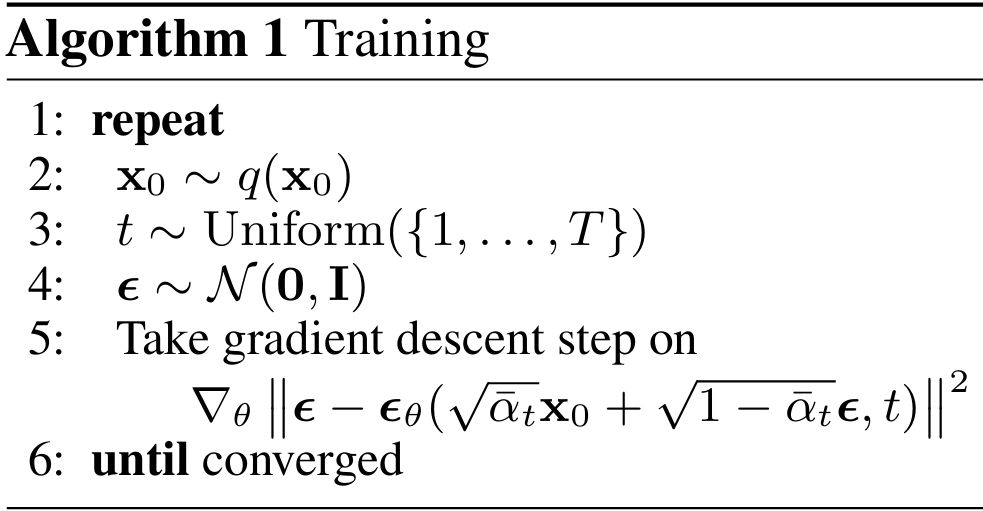
\includegraphics[width=\textwidth]{image/pseudo1.png}
        \caption{Pseudocode 1}
    \end{minipage}
    \hfill
    \begin{minipage}{0.5\textwidth}
        \centering
        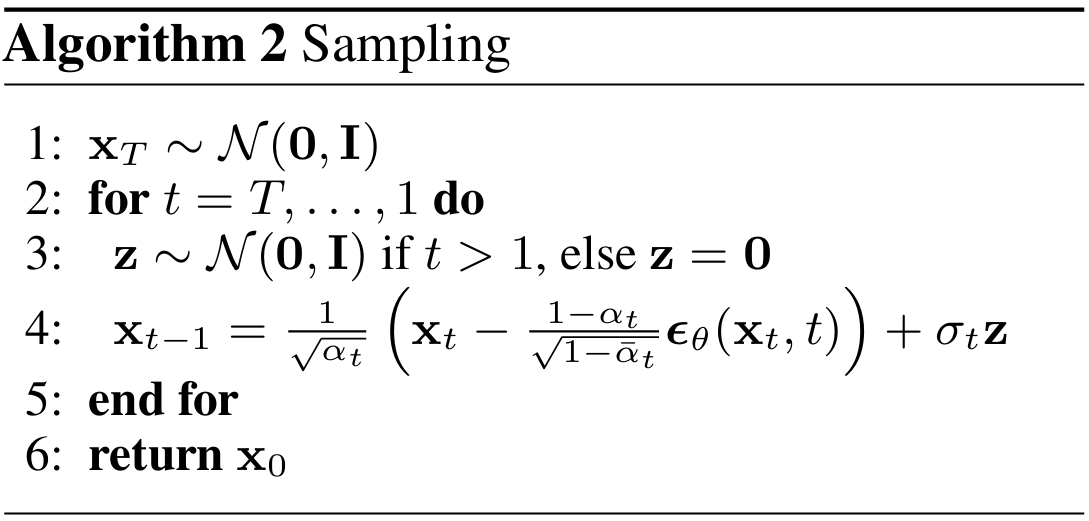
\includegraphics[width=\textwidth]{image/pseudo2.png}
        \caption{Pseudocode 2}
    \end{minipage}
\end{figure}

In the pseudocode above, \(\alpha_t = 1-\beta_t\),
\(\overline{\alpha_t} = \prod_{s-1}^t \alpha_s\), where \(\beta\)
denotes the beta schedule which increases linearly. \(\epsilon\) denotes
noise and \(x_0\) denotes the original data, meanwhile \(x_T\) denotes
that generated noise under normal distribution. Here we will apply the
algorithm above to our specific task.\\
The data stream and network component is presented in the figure below:

\begin{figure}
    \centering
    \begin{minipage}{0.5\textwidth}
        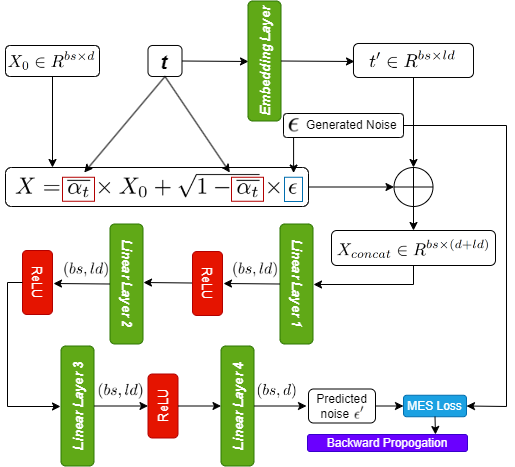
\includegraphics[width=\textwidth]{image/training_network.png}
        \caption{Training Network}
    \end{minipage}
\end{figure}

In the figure of training, \(X_0 \in R^{bs \times d}\) is the input data
distribution where \(bs\) denotes batch size and \(d\) denotes the
dimension of the input data. Using the generated noise \(\epsilon\) and
the original batch data under specific proportion, a noised sample is
generated. The randomly chosen specific timestep t is embedded into
latent space of dimension \(ld\), and it will be concatenated with the
noised sample. It should be noted that \(ld\) is actually a
hyperparameter. Then the concatenated tensor will be processed by three
blocks which individually consists of a Linear Layer and a ReLU
activation funcion. Finally, the processed tensor will be projected to
the wanted dimension \(d\) and is expected to be a close simulation of
the original generated noise \(\epsilon\). Here we use the MSE Loss as
the loss function for backpropogation. We emphasize that during
training, the time step t is randomly chosen, not orderly chosen, so as
to fully maximize every batch of data since in this way every batch data
can be cooperated with a different timestep t which, to some extent,
improve the robustness of the network. The noise predictor in this
implementation consists of four linear layers, three activation
functions, and involves an embedding layer for projecting discrete
timestep into continuous latent space.

\begin{figure}
    \centering
    \begin{minipage}{0.8\textwidth}
        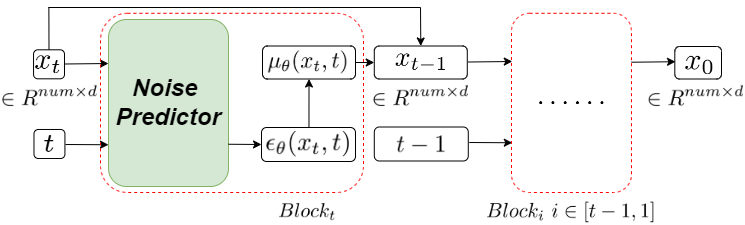
\includegraphics[width=\textwidth]{image/sampling.png}
        \caption{Sampling Network}
    \end{minipage}
\end{figure}

In the figure of sampling presented above, we firstly generate a noise tensor with
dimension \(num \times d\), which subdues normal dirtribution. Then
starting from the timestep t to 1, we will input the noised distribution
and the timestep into the noise predictor to generated a simulated
noise. Then we will use the noised data and simulated noise to generated
the data one step ahead, in the proportion illustrated in the pseudocode
of sampling. The generated \(X_{t-1}\) will be the input of the next
block, together with timestep \(t-1\) correspondingly. This process will
be repeated \(t\) times until \(X_0\) is generated, which should be
expected to yield the same distribution of the input data.

    \subsection*{5.3 Experiment}\label{experiment}

Unless additionally stated, we set up 4000 epochs and 100 timesteps. The
dimension of the hidden space for timestep \(t\) is 128, and the batch
size is set to 32 with dataloader's shuffling mode on. It is noticeable
that the timestep isn't rather large, since it is generally considered
that the data distribution is not way too complicated and excessive
training and inferencing isn't necessary. \#\#\# Result and
Visualization on 3D Experiment We train our model on the dataset of
\(R^{100, 3}\), i.e., on the dataset consisting of 100 data on 3
people's money while the total amount of money is 5, specifically
speaking. Since the data visualization for three dimensional dataset is
quite accessable, here we visualize the data distribution of the
original dataset and generated dataset that comprises 1000 pieces of
data, respectively. The visualization code is presented in Appendix.B.
Note that the figures of visualization are from the result we run on our
computer, not this Jupyter Notebook. You can use the visualization code
in Appendix.A and the `simulated\_data\_from\_raw\_1.npy' file this
jupyter created to visualize it yourself.

\begin{figure}[H]
    \centering
    \begin{minipage}{0.3\textwidth}
        \centering
        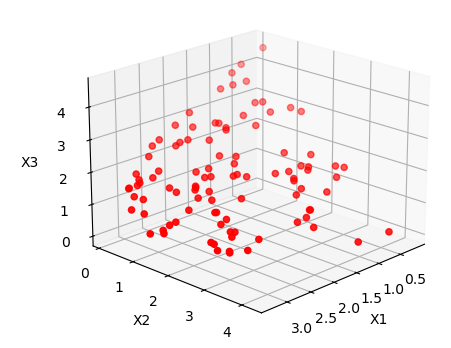
\includegraphics[width=\textwidth]{image/vis_collected.png}
    \end{minipage}
    \hfill
    \begin{minipage}{0.3\textwidth}
        \centering
        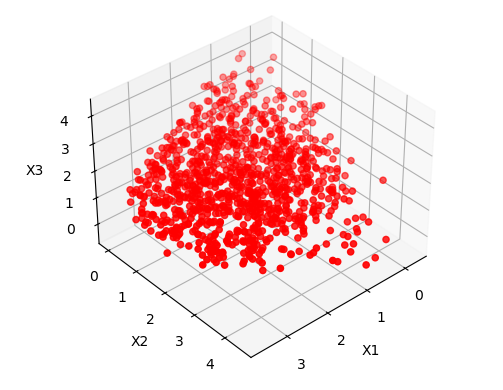
\includegraphics[width=\textwidth]{image/dif_col_generated_1.png}
    \end{minipage}
    \hfill
    \begin{minipage}{0.3\textwidth}
        \centering
        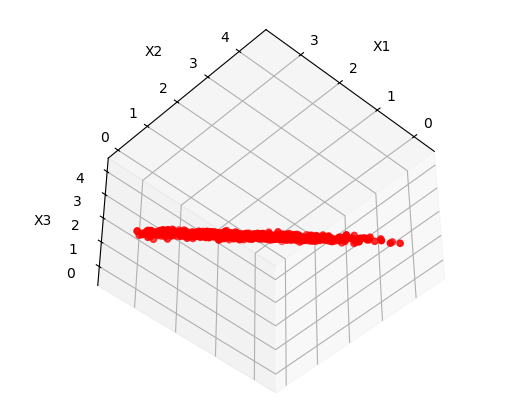
\includegraphics[width=\textwidth]{image/dif_col_generated_2.png}
    \end{minipage}
\end{figure}

From the figure above, starting from left to right, the pictures are
about the visualization for the original data, the visualization the
generated data, and another view into the visualization of the generated
data. It is manifest that the simulated data subdues the distribution of
the orignal data well, which is indicated by the tiny jittering of the
plane in the figure. This is intuitive that the simulation is quite good
since the hidden distribution of the original data is not obscure, and
the network can easily learn the linear paterns behind the data. Not to
further mention that the data is only three dimensional.

    \subsection*{5.4 Result and Visualization on 4D experiment}\label{result-and-visualization-on-4d-experiment}

We also train our model on a (100, 4) dataset. Since it is hard to do
visualization for 4 dimensional data, we convert the npy file to csv and
further do Kolmogorov-Smirnov Test. The code and test results are
presented below, indicating that the newly generated data share the same
latent distribution with the old collected data.

\begin{tcolorbox}[breakable, size=fbox, boxrule=1pt, pad at break*=1mm,colback=cellbackground, colframe=cellborder]
\prompt{In}{incolor}{8}{\boxspacing}
\begin{Verbatim}[commandchars=\\\{\}]
\PY{n}{data} \PY{o}{=} \PY{n}{np}\PY{o}{.}\PY{n}{load}\PY{p}{(}\PY{l+s+s1}{\PYZsq{}}\PY{l+s+s1}{data/simulated\PYZus{}data\PYZus{}from\PYZus{}raw\PYZus{}2\PYZus{}not\PYZus{}ipynb.npy}\PY{l+s+s1}{\PYZsq{}}\PY{p}{)}  
\PY{n+nb}{print}\PY{p}{(}\PY{l+s+s2}{\PYZdq{}}\PY{l+s+s2}{There are totally}\PY{l+s+s2}{\PYZdq{}}\PY{p}{,} \PY{n}{data}\PY{o}{.}\PY{n}{shape}\PY{p}{[}\PY{l+m+mi}{0}\PY{p}{]}\PY{p}{,} \PY{l+s+s2}{\PYZdq{}}\PY{l+s+s2}{pieces of samples, and there are}\PY{l+s+s2}{\PYZdq{}}\PY{p}{,} \PY{n}{data}\PY{o}{.}\PY{n}{shape}\PY{p}{[}\PY{l+m+mi}{1}\PY{p}{]}\PY{p}{,} \PY{l+s+s2}{\PYZdq{}}\PY{l+s+s2}{people in total.}\PY{l+s+s2}{\PYZdq{}}\PY{p}{)}

\PY{n}{df} \PY{o}{=} \PY{n}{pd}\PY{o}{.}\PY{n}{DataFrame}\PY{p}{(}\PY{n}{data}\PY{p}{)}

\PY{n}{df}\PY{o}{.}\PY{n}{to\PYZus{}csv}\PY{p}{(}\PY{l+s+s1}{\PYZsq{}}\PY{l+s+s1}{data/csv/diffusion\PYZus{}generated\PYZus{}four.csv}\PY{l+s+s1}{\PYZsq{}}\PY{p}{,} \PY{n}{index}\PY{o}{=}\PY{k+kc}{False}\PY{p}{)} 

\PY{c+c1}{\PYZsh{} Perform the comparison}
\PY{n}{results} \PY{o}{=} \PY{n}{compare\PYZus{}distributions}\PY{p}{(}\PY{l+s+s1}{\PYZsq{}}\PY{l+s+s1}{data/csv/data2.csv}\PY{l+s+s1}{\PYZsq{}}\PY{p}{,} \PY{l+s+s1}{\PYZsq{}}\PY{l+s+s1}{data/csv/diffusion\PYZus{}generated\PYZus{}four.csv}\PY{l+s+s1}{\PYZsq{}}\PY{p}{)}

\PY{c+c1}{\PYZsh{} Print detailed results}
\PY{n+nb}{print}\PY{p}{(}\PY{l+s+s2}{\PYZdq{}}\PY{l+s+s2}{Kolmogorov\PYZhy{}Smirnov Test Results:}\PY{l+s+s2}{\PYZdq{}}\PY{p}{)}
\PY{k}{for} \PY{n}{column}\PY{p}{,} \PY{n}{result} \PY{o+ow}{in} \PY{n}{results}\PY{o}{.}\PY{n}{items}\PY{p}{(}\PY{p}{)}\PY{p}{:}
    \PY{n+nb}{print}\PY{p}{(}\PY{l+s+sa}{f}\PY{l+s+s2}{\PYZdq{}}\PY{l+s+se}{\PYZbs{}n}\PY{l+s+s2}{\PYZhy{} **Column }\PY{l+s+si}{\PYZob{}}\PY{n}{column}\PY{l+s+si}{\PYZcb{}}\PY{l+s+s2}{**:}\PY{l+s+s2}{\PYZdq{}}\PY{p}{)}
    \PY{n+nb}{print}\PY{p}{(}\PY{l+s+sa}{f}\PY{l+s+s2}{\PYZdq{}}\PY{l+s+s2}{  \PYZhy{} KS Statistic: }\PY{l+s+si}{\PYZob{}}\PY{n}{result}\PY{p}{[}\PY{l+s+s1}{\PYZsq{}}\PY{l+s+s1}{statistic}\PY{l+s+s1}{\PYZsq{}}\PY{p}{]}\PY{l+s+si}{\PYZcb{}}\PY{l+s+s2}{\PYZdq{}}\PY{p}{)}
    \PY{n+nb}{print}\PY{p}{(}\PY{l+s+sa}{f}\PY{l+s+s2}{\PYZdq{}}\PY{l+s+s2}{  \PYZhy{} P\PYZhy{}value: }\PY{l+s+si}{\PYZob{}}\PY{n}{result}\PY{p}{[}\PY{l+s+s1}{\PYZsq{}}\PY{l+s+s1}{p\PYZus{}value}\PY{l+s+s1}{\PYZsq{}}\PY{p}{]}\PY{l+s+si}{\PYZcb{}}\PY{l+s+s2}{\PYZdq{}}\PY{p}{)}
    \PY{n+nb}{print}\PY{p}{(}\PY{l+s+sa}{f}\PY{l+s+s2}{\PYZdq{}}\PY{l+s+s2}{  \PYZhy{} Significant Difference: }\PY{l+s+si}{\PYZob{}}\PY{l+s+s1}{\PYZsq{}}\PY{l+s+s1}{Yes}\PY{l+s+s1}{\PYZsq{}}\PY{+w}{ }\PY{k}{if}\PY{+w}{ }\PY{n}{result}\PY{p}{[}\PY{l+s+s1}{\PYZsq{}}\PY{l+s+s1}{significant\PYZus{}diff}\PY{l+s+s1}{\PYZsq{}}\PY{p}{]}\PY{+w}{ }\PY{k}{else}\PY{+w}{ }\PY{l+s+s1}{\PYZsq{}}\PY{l+s+s1}{No}\PY{l+s+s1}{\PYZsq{}}\PY{l+s+si}{\PYZcb{}}\PY{l+s+s2}{\PYZdq{}}\PY{p}{)}

\PY{c+c1}{\PYZsh{} Additional interpretation}
\PY{n}{significant\PYZus{}columns} \PY{o}{=} \PY{p}{[}\PY{n}{col} \PY{k}{for} \PY{n}{col}\PY{p}{,} \PY{n}{res} \PY{o+ow}{in} \PY{n}{results}\PY{o}{.}\PY{n}{items}\PY{p}{(}\PY{p}{)} \PY{k}{if} \PY{n}{res}\PY{p}{[}\PY{l+s+s1}{\PYZsq{}}\PY{l+s+s1}{significant\PYZus{}diff}\PY{l+s+s1}{\PYZsq{}}\PY{p}{]}\PY{p}{]}
\PY{n+nb}{print}\PY{p}{(}\PY{l+s+s2}{\PYZdq{}}\PY{l+s+se}{\PYZbs{}n}\PY{l+s+s2}{Conclusion:}\PY{l+s+s2}{\PYZdq{}}\PY{p}{)}
\PY{k}{if} \PY{o+ow}{not} \PY{n}{significant\PYZus{}columns}\PY{p}{:}
    \PY{n+nb}{print}\PY{p}{(}\PY{l+s+s2}{\PYZdq{}}\PY{l+s+s2}{All columns have p\PYZhy{}values greater than 0.05, so we cannot reject the null hypothesis. This indicates no significant distribution differences between actual measurements and ideal simulations across the columns.}\PY{l+s+s2}{\PYZdq{}}\PY{p}{)}
\PY{k}{else}\PY{p}{:}
    \PY{n+nb}{print}\PY{p}{(}\PY{l+s+sa}{f}\PY{l+s+s2}{\PYZdq{}}\PY{l+s+s2}{Columns }\PY{l+s+si}{\PYZob{}}\PY{l+s+s1}{\PYZsq{}}\PY{l+s+s1}{, }\PY{l+s+s1}{\PYZsq{}}\PY{o}{.}\PY{n}{join}\PY{p}{(}\PY{n+nb}{map}\PY{p}{(}\PY{n+nb}{str}\PY{p}{,}\PY{+w}{ }\PY{n}{significant\PYZus{}columns}\PY{p}{)}\PY{p}{)}\PY{l+s+si}{\PYZcb{}}\PY{l+s+s2}{ show significant distribution differences. Other columns do not have significant differences.}\PY{l+s+s2}{\PYZdq{}}\PY{p}{)}
\end{Verbatim}
\end{tcolorbox}

    \begin{Verbatim}[commandchars=\\\{\}]
There are totally 1000 pieces of samples, and there are 4 people in total.
Kolmogorov-Smirnov Test Results:

- **Column 0**:
  - KS Statistic: 0.0636
  - P-value: 0.8349
  - Significant Difference: No

- **Column 1**:
  - KS Statistic: 0.0694
  - P-value: 0.7501
  - Significant Difference: No

- **Column 2**:
  - KS Statistic: 0.1262
  - P-value: 0.1036
  - Significant Difference: No

- **Column 3**:
  - KS Statistic: 0.1064
  - P-value: 0.2403
  - Significant Difference: No

Conclusion:
All columns have p-values greater than 0.05, so we cannot reject the null
hypothesis. This indicates no significant distribution differences between
actual measurements and ideal simulations across the columns.
    \end{Verbatim}

    \section*{6. Further Discussion and Theoretical Analysis}\label{further-discussion-and-theoretical-analysis}

\subsection*{6.1 Clicking Strategy}\label{clicking-strategy}

Since the expectation money of each person is identical which is proved
in Appendix.C, so actually when the number of clicked red envelope
containing the same total money grows to infinity, the expectation will
always be the same. But it can be proved that: the later you click the
envelope, the higher your money variance is. The proof is presented in
Appendix.C. So if you want to take risks to receive more money
relatively to others, you can click the red envelope later. Meanwhile,
if you want to secure median amount of money and you are satisfied with
it, you can click the red envelop as early as possible. In this
strategy, the number of people in Wechat Group and the number of people
who have already obtained the red envelope doesn't matter. The only
decision you have to make is about how soon or how late you will click
the red envelope.

\subsection*{6.2 Holiday Factor}

Will the distribution change
when it comes to special days? Intuitively, this shouldn't be true.
Still, we collected additional datesets on Jan 1st, 2025, with 5 yuan in
total, 25 trials, three or four people respectively. Then we will run
only Kolmogorov-Smirnov test on these two datasets since the sample
number is too small.

The result on the data containing three people:

    \begin{tcolorbox}[breakable, size=fbox, boxrule=1pt, pad at break*=1mm,colback=cellbackground, colframe=cellborder]
\prompt{In}{incolor}{28}{\boxspacing}
\begin{Verbatim}[commandchars=\\\{\}]
\PY{c+c1}{\PYZsh{} Perform the comparison}
\PY{n}{results} \PY{o}{=} \PY{n}{compare\PYZus{}distributions}\PY{p}{(}\PY{l+s+s1}{\PYZsq{}}\PY{l+s+s1}{data/csv/data1.csv}\PY{l+s+s1}{\PYZsq{}}\PY{p}{,} \PY{l+s+s1}{\PYZsq{}}\PY{l+s+s1}{data/csv/data4.csv}\PY{l+s+s1}{\PYZsq{}}\PY{p}{)}

\PY{c+c1}{\PYZsh{} Print detailed results}
\PY{n+nb}{print}\PY{p}{(}\PY{l+s+s2}{\PYZdq{}}\PY{l+s+s2}{Kolmogorov\PYZhy{}Smirnov Test Results:}\PY{l+s+s2}{\PYZdq{}}\PY{p}{)}
\PY{k}{for} \PY{n}{column}\PY{p}{,} \PY{n}{result} \PY{o+ow}{in} \PY{n}{results}\PY{o}{.}\PY{n}{items}\PY{p}{(}\PY{p}{)}\PY{p}{:}
    \PY{n+nb}{print}\PY{p}{(}\PY{l+s+sa}{f}\PY{l+s+s2}{\PYZdq{}}\PY{l+s+se}{\PYZbs{}n}\PY{l+s+s2}{\PYZhy{} **Column }\PY{l+s+si}{\PYZob{}}\PY{n}{column}\PY{l+s+si}{\PYZcb{}}\PY{l+s+s2}{**:}\PY{l+s+s2}{\PYZdq{}}\PY{p}{)}
    \PY{n+nb}{print}\PY{p}{(}\PY{l+s+sa}{f}\PY{l+s+s2}{\PYZdq{}}\PY{l+s+s2}{  \PYZhy{} KS Statistic: }\PY{l+s+si}{\PYZob{}}\PY{n}{result}\PY{p}{[}\PY{l+s+s1}{\PYZsq{}}\PY{l+s+s1}{statistic}\PY{l+s+s1}{\PYZsq{}}\PY{p}{]}\PY{l+s+si}{\PYZcb{}}\PY{l+s+s2}{\PYZdq{}}\PY{p}{)}
    \PY{n+nb}{print}\PY{p}{(}\PY{l+s+sa}{f}\PY{l+s+s2}{\PYZdq{}}\PY{l+s+s2}{  \PYZhy{} P\PYZhy{}value: }\PY{l+s+si}{\PYZob{}}\PY{n}{result}\PY{p}{[}\PY{l+s+s1}{\PYZsq{}}\PY{l+s+s1}{p\PYZus{}value}\PY{l+s+s1}{\PYZsq{}}\PY{p}{]}\PY{l+s+si}{\PYZcb{}}\PY{l+s+s2}{\PYZdq{}}\PY{p}{)}
    \PY{n+nb}{print}\PY{p}{(}\PY{l+s+sa}{f}\PY{l+s+s2}{\PYZdq{}}\PY{l+s+s2}{  \PYZhy{} Significant Difference: }\PY{l+s+si}{\PYZob{}}\PY{l+s+s1}{\PYZsq{}}\PY{l+s+s1}{Yes}\PY{l+s+s1}{\PYZsq{}}\PY{+w}{ }\PY{k}{if}\PY{+w}{ }\PY{n}{result}\PY{p}{[}\PY{l+s+s1}{\PYZsq{}}\PY{l+s+s1}{significant\PYZus{}diff}\PY{l+s+s1}{\PYZsq{}}\PY{p}{]}\PY{+w}{ }\PY{k}{else}\PY{+w}{ }\PY{l+s+s1}{\PYZsq{}}\PY{l+s+s1}{No}\PY{l+s+s1}{\PYZsq{}}\PY{l+s+si}{\PYZcb{}}\PY{l+s+s2}{\PYZdq{}}\PY{p}{)}

\PY{c+c1}{\PYZsh{} Additional interpretation}
\PY{n}{significant\PYZus{}columns} \PY{o}{=} \PY{p}{[}\PY{n}{col} \PY{k}{for} \PY{n}{col}\PY{p}{,} \PY{n}{res} \PY{o+ow}{in} \PY{n}{results}\PY{o}{.}\PY{n}{items}\PY{p}{(}\PY{p}{)} \PY{k}{if} \PY{n}{res}\PY{p}{[}\PY{l+s+s1}{\PYZsq{}}\PY{l+s+s1}{significant\PYZus{}diff}\PY{l+s+s1}{\PYZsq{}}\PY{p}{]}\PY{p}{]}
\PY{n+nb}{print}\PY{p}{(}\PY{l+s+s2}{\PYZdq{}}\PY{l+s+se}{\PYZbs{}n}\PY{l+s+s2}{Conclusion:}\PY{l+s+s2}{\PYZdq{}}\PY{p}{)}
\PY{k}{if} \PY{o+ow}{not} \PY{n}{significant\PYZus{}columns}\PY{p}{:}
    \PY{n+nb}{print}\PY{p}{(}\PY{l+s+s2}{\PYZdq{}}\PY{l+s+s2}{All columns have p\PYZhy{}values greater than 0.05, so we cannot reject the null hypothesis. This indicates no significant distribution differences between actual measurements and ideal simulations across the columns.}\PY{l+s+s2}{\PYZdq{}}\PY{p}{)}
\PY{k}{else}\PY{p}{:}
    \PY{n+nb}{print}\PY{p}{(}\PY{l+s+sa}{f}\PY{l+s+s2}{\PYZdq{}}\PY{l+s+s2}{Columns }\PY{l+s+si}{\PYZob{}}\PY{l+s+s1}{\PYZsq{}}\PY{l+s+s1}{, }\PY{l+s+s1}{\PYZsq{}}\PY{o}{.}\PY{n}{join}\PY{p}{(}\PY{n+nb}{map}\PY{p}{(}\PY{n+nb}{str}\PY{p}{,}\PY{+w}{ }\PY{n}{significant\PYZus{}columns}\PY{p}{)}\PY{p}{)}\PY{l+s+si}{\PYZcb{}}\PY{l+s+s2}{ show significant distribution differences. Other columns do not have significant differences.}\PY{l+s+s2}{\PYZdq{}}\PY{p}{)}
\end{Verbatim}
\end{tcolorbox}

    \begin{Verbatim}[commandchars=\\\{\}]
Kolmogorov-Smirnov Test Results:

- **Column 0**:
  - KS Statistic: 0.1833
  - P-value: 0.4741
  - Significant Difference: No

- **Column 1**:
  - KS Statistic: 0.2467
  - P-value: 0.1588
  - Significant Difference: No

- **Column 2**:
  - KS Statistic: 0.21
  - P-value: 0.3121
  - Significant Difference: No

Conclusion:
All columns have p-values greater than 0.05, so we cannot reject the null
hypothesis. This indicates no significant distribution differences between
actual measurements and ideal simulations across the columns.
    \end{Verbatim}

    The result on the data containing four people:

    \begin{tcolorbox}[breakable, size=fbox, boxrule=1pt, pad at break*=1mm,colback=cellbackground, colframe=cellborder]
\prompt{In}{incolor}{29}{\boxspacing}
\begin{Verbatim}[commandchars=\\\{\}]
\PY{c+c1}{\PYZsh{} Perform the comparison}
\PY{n}{results} \PY{o}{=} \PY{n}{compare\PYZus{}distributions}\PY{p}{(}\PY{l+s+s1}{\PYZsq{}}\PY{l+s+s1}{data/csv/data2.csv}\PY{l+s+s1}{\PYZsq{}}\PY{p}{,} \PY{l+s+s1}{\PYZsq{}}\PY{l+s+s1}{data/csv/data5.csv}\PY{l+s+s1}{\PYZsq{}}\PY{p}{)}

\PY{c+c1}{\PYZsh{} Print detailed results}
\PY{n+nb}{print}\PY{p}{(}\PY{l+s+s2}{\PYZdq{}}\PY{l+s+s2}{Kolmogorov\PYZhy{}Smirnov Test Results:}\PY{l+s+s2}{\PYZdq{}}\PY{p}{)}
\PY{k}{for} \PY{n}{column}\PY{p}{,} \PY{n}{result} \PY{o+ow}{in} \PY{n}{results}\PY{o}{.}\PY{n}{items}\PY{p}{(}\PY{p}{)}\PY{p}{:}
    \PY{n+nb}{print}\PY{p}{(}\PY{l+s+sa}{f}\PY{l+s+s2}{\PYZdq{}}\PY{l+s+se}{\PYZbs{}n}\PY{l+s+s2}{\PYZhy{} **Column }\PY{l+s+si}{\PYZob{}}\PY{n}{column}\PY{l+s+si}{\PYZcb{}}\PY{l+s+s2}{**:}\PY{l+s+s2}{\PYZdq{}}\PY{p}{)}
    \PY{n+nb}{print}\PY{p}{(}\PY{l+s+sa}{f}\PY{l+s+s2}{\PYZdq{}}\PY{l+s+s2}{  \PYZhy{} KS Statistic: }\PY{l+s+si}{\PYZob{}}\PY{n}{result}\PY{p}{[}\PY{l+s+s1}{\PYZsq{}}\PY{l+s+s1}{statistic}\PY{l+s+s1}{\PYZsq{}}\PY{p}{]}\PY{l+s+si}{\PYZcb{}}\PY{l+s+s2}{\PYZdq{}}\PY{p}{)}
    \PY{n+nb}{print}\PY{p}{(}\PY{l+s+sa}{f}\PY{l+s+s2}{\PYZdq{}}\PY{l+s+s2}{  \PYZhy{} P\PYZhy{}value: }\PY{l+s+si}{\PYZob{}}\PY{n}{result}\PY{p}{[}\PY{l+s+s1}{\PYZsq{}}\PY{l+s+s1}{p\PYZus{}value}\PY{l+s+s1}{\PYZsq{}}\PY{p}{]}\PY{l+s+si}{\PYZcb{}}\PY{l+s+s2}{\PYZdq{}}\PY{p}{)}
    \PY{n+nb}{print}\PY{p}{(}\PY{l+s+sa}{f}\PY{l+s+s2}{\PYZdq{}}\PY{l+s+s2}{  \PYZhy{} Significant Difference: }\PY{l+s+si}{\PYZob{}}\PY{l+s+s1}{\PYZsq{}}\PY{l+s+s1}{Yes}\PY{l+s+s1}{\PYZsq{}}\PY{+w}{ }\PY{k}{if}\PY{+w}{ }\PY{n}{result}\PY{p}{[}\PY{l+s+s1}{\PYZsq{}}\PY{l+s+s1}{significant\PYZus{}diff}\PY{l+s+s1}{\PYZsq{}}\PY{p}{]}\PY{+w}{ }\PY{k}{else}\PY{+w}{ }\PY{l+s+s1}{\PYZsq{}}\PY{l+s+s1}{No}\PY{l+s+s1}{\PYZsq{}}\PY{l+s+si}{\PYZcb{}}\PY{l+s+s2}{\PYZdq{}}\PY{p}{)}

\PY{c+c1}{\PYZsh{} Additional interpretation}
\PY{n}{significant\PYZus{}columns} \PY{o}{=} \PY{p}{[}\PY{n}{col} \PY{k}{for} \PY{n}{col}\PY{p}{,} \PY{n}{res} \PY{o+ow}{in} \PY{n}{results}\PY{o}{.}\PY{n}{items}\PY{p}{(}\PY{p}{)} \PY{k}{if} \PY{n}{res}\PY{p}{[}\PY{l+s+s1}{\PYZsq{}}\PY{l+s+s1}{significant\PYZus{}diff}\PY{l+s+s1}{\PYZsq{}}\PY{p}{]}\PY{p}{]}
\PY{n+nb}{print}\PY{p}{(}\PY{l+s+s2}{\PYZdq{}}\PY{l+s+se}{\PYZbs{}n}\PY{l+s+s2}{Conclusion:}\PY{l+s+s2}{\PYZdq{}}\PY{p}{)}
\PY{k}{if} \PY{o+ow}{not} \PY{n}{significant\PYZus{}columns}\PY{p}{:}
    \PY{n+nb}{print}\PY{p}{(}\PY{l+s+s2}{\PYZdq{}}\PY{l+s+s2}{All columns have p\PYZhy{}values greater than 0.05, so we cannot reject the null hypothesis. This indicates no significant distribution differences between actual measurements and ideal simulations across the columns.}\PY{l+s+s2}{\PYZdq{}}\PY{p}{)}
\PY{k}{else}\PY{p}{:}
    \PY{n+nb}{print}\PY{p}{(}\PY{l+s+sa}{f}\PY{l+s+s2}{\PYZdq{}}\PY{l+s+s2}{Columns }\PY{l+s+si}{\PYZob{}}\PY{l+s+s1}{\PYZsq{}}\PY{l+s+s1}{, }\PY{l+s+s1}{\PYZsq{}}\PY{o}{.}\PY{n}{join}\PY{p}{(}\PY{n+nb}{map}\PY{p}{(}\PY{n+nb}{str}\PY{p}{,}\PY{+w}{ }\PY{n}{significant\PYZus{}columns}\PY{p}{)}\PY{p}{)}\PY{l+s+si}{\PYZcb{}}\PY{l+s+s2}{ show significant distribution differences. Other columns do not have significant differences.}\PY{l+s+s2}{\PYZdq{}}\PY{p}{)}
\end{Verbatim}
\end{tcolorbox}

    \begin{Verbatim}[commandchars=\\\{\}]
Kolmogorov-Smirnov Test Results:

- **Column 0**:
  - KS Statistic: 0.3081
  - P-value: 0.0398
  - Significant Difference: Yes

- **Column 1**:
  - KS Statistic: 0.2513
  - P-value: 0.1443
  - Significant Difference: No

- **Column 2**:
  - KS Statistic: 0.1098
  - P-value: 0.9503
  - Significant Difference: No

- **Column 3**:
  - KS Statistic: 0.2652
  - P-value: 0.1084
  - Significant Difference: No

Conclusion:
Columns 0 show significant distribution differences. Other columns do not have
significant differences.
    \end{Verbatim}

    The result below hints that the distribution are the same, no matter
whether it is a special day or not. Note that in the result of four
people, p-value equals 0.04, which is slightly smaller than 0.05. This
is considered normal since the number of sample is small, and the money
distribution of the first people is purely randomly distributed. In
conclusion, we tend to disagree that holiday could be a possible factor
effecting the data distribution

    \subsubsection*{6.3 User-Specific Mechanism}\label{user-specific-mechanism}

Consider a special Wechat Group, where everyone want to have rather
considerable amount of money when receiving red envelopes, or someone is
a super vip and should receive more money. This requires the algorithm
to have control over the overall distribution robustly. We deesign the
following algorithm. Assuming there are N people and M yuan: \[
Y_1, Y_2, \dots, Y_n \sim N(0, \sigma ^2)
\] \[
w_1, w_2, \dots, w_n \in \mathbf{R^+}
\] \[
X_i = N\frac{w_iY_i}{\sum_{i=1}^N Y_i}
\] where \(\sigma, w_i\) are hyperparameters. The \(i-th\) person ,
whose weight is \(w_i\), will take away the number according to his
weight index, i.e., \(X_i\). Note that in this algorithm, the numbers
are determined previously. We use \(\sigma\) to control the initial
variance of data distribution, and we use \(w_i\) to designate weight to
each individual. For instance, Pony is a VVVIP user of Penguin social
app, and Penguin company have rule that VVVIP will have more money when
receiving envelope. Therefore we can set \(w_{\text{pony}}\) relatively rather
large. When Pony click the red envelope, he takes away \(X_{\text{pony}}\)
yuan, whose weight is \(w_{\text{pony}}\). For another example, for a group of
children, since we don't want to break their heart, we want to share the
money as fair as possible. We can set \(\sigma\) rather small, and set
there weights \(w_i\) identical.

\section*{7. Limitation}

This work mainly elaborate on the possible model of data distribution and focus on the application of diffusion model. Still we believe that there are some limitations of this report. 

\begin{itemize}
    \item Shortage of Dataset: The process of data collecting is time-comsuming and exhausting. Due to lack of ample time, we are only able to collect two main datasets and two additional datasets for discussion of holiday factors. Generally speaking, the more samples we have, the better it is. Fortunately that the data distribution are strictly executed during clicking the red envelopes and the distribution pattern are not complicated and as a result the diffusion model can converge to this pattern easily.
    \item More Possible Factors: In this work, we only concentrate on the topic that whether the holiday is going to change the distribution, but in fact there are lots of potential factors. There are other probable factors like the number of people in the group, whether users are abroad, are not covered in this report. Moreover, we only test on the New Year's Day, so jumping to the conclusion that holiday isn't a factor may be inaccurate.
    \item Generalizations: There are Red Envelope everywhere, like QQ (Penguin Company), Tiktok, etc. It is also an intriguing topic about whether all the red envelope in other platforms share the same mechanism as Wechat's. The generalization of Double Expectation Algorithm are still yet to be verified.
\end{itemize}

\section*{Conclusion}

In this report, we delve into the hidden distribution mechanism of Wechat Red Envelope. We first try to use traditional distribution models to fit the data, but all the results are far from satisfaction. Then according to some key observations and assumptions, inspired by some previous related blogs or work, Double Expectation Model is proposed. We run Chi-Square test and Kolmogorov-Smirnov test to testify the matching degree of our model. Additionally, we use the latest diffusion model to learn the data distribution and further generate more data. We run the verification test on the generated data as well, indicating that the model has learned the latent distribution well. Finally, we discussed further on clicking strategy, possible factors, and possibly more robust distribution algorithm.

\section*{Appendix}\label{appendix}

\subsection*{A. Visualization Code}\label{a.-visualization-code}

\begin{tcolorbox}[breakable, size=fbox, boxrule=1pt, pad at break*=1mm,colback=cellbackground, colframe=cellborder]
\prompt{In}{incolor}{ }{\boxspacing}
\begin{Verbatim}[commandchars=\\\{\}]
\PY{k+kn}{import} \PY{n+nn}{torch}
\PY{k+kn}{import} \PY{n+nn}{matplotlib}\PY{n+nn}{.}\PY{n+nn}{pyplot} \PY{k}{as} \PY{n+nn}{plt}
\PY{k+kn}{import} \PY{n+nn}{numpy} \PY{k}{as} \PY{n+nn}{np}

\PY{n}{data} \PY{o}{=} \PY{n}{np}\PY{o}{.}\PY{n}{load}\PY{p}{(}\PY{l+s+s1}{\PYZsq{}}\PY{l+s+s1}{code/data/toy.npy}\PY{l+s+s1}{\PYZsq{}}\PY{p}{)}
\PY{n+nb}{print}\PY{p}{(}\PY{n}{data}\PY{o}{.}\PY{n}{shape}\PY{p}{)}
\PY{n}{data} \PY{o}{=} \PY{n}{data}\PY{p}{[}\PY{p}{:}\PY{p}{,} \PY{p}{:}\PY{l+m+mi}{3}\PY{p}{]}
\PY{c+c1}{\PYZsh{} Data preprocessing}
\PY{n}{dataset} \PY{o}{=} \PY{n}{torch}\PY{o}{.}\PY{n}{Tensor}\PY{p}{(}\PY{n}{data}\PY{p}{)}\PY{o}{.}\PY{n}{float}\PY{p}{(}\PY{p}{)}  \PY{c+c1}{\PYZsh{} shape: (10000, 3)}

\PY{c+c1}{\PYZsh{} Visualize data}
\PY{n}{fig} \PY{o}{=} \PY{n}{plt}\PY{o}{.}\PY{n}{figure}\PY{p}{(}\PY{p}{)}
\PY{n}{ax} \PY{o}{=} \PY{n}{fig}\PY{o}{.}\PY{n}{add\PYZus{}subplot}\PY{p}{(}\PY{l+m+mi}{111}\PY{p}{,} \PY{n}{projection}\PY{o}{=}\PY{l+s+s1}{\PYZsq{}}\PY{l+s+s1}{3d}\PY{l+s+s1}{\PYZsq{}}\PY{p}{)}
\PY{n}{ax}\PY{o}{.}\PY{n}{scatter}\PY{p}{(}\PY{n}{data}\PY{p}{[}\PY{p}{:}\PY{p}{,} \PY{l+m+mi}{0}\PY{p}{]}\PY{p}{,} \PY{n}{data}\PY{p}{[}\PY{p}{:}\PY{p}{,} \PY{l+m+mi}{1}\PY{p}{]}\PY{p}{,} \PY{n}{data}\PY{p}{[}\PY{p}{:}\PY{p}{,} \PY{l+m+mi}{2}\PY{p}{]}\PY{p}{,} \PY{n}{color}\PY{o}{=}\PY{l+s+s1}{\PYZsq{}}\PY{l+s+s1}{red}\PY{l+s+s1}{\PYZsq{}}\PY{p}{,} \PY{n}{s}\PY{o}{=}\PY{l+m+mi}{10}\PY{p}{,} \PY{n}{edgecolors}\PY{o}{=}\PY{l+s+s1}{\PYZsq{}}\PY{l+s+s1}{black}\PY{l+s+s1}{\PYZsq{}}\PY{p}{)}
\PY{n}{ax}\PY{o}{.}\PY{n}{set\PYZus{}xlabel}\PY{p}{(}\PY{l+s+s1}{\PYZsq{}}\PY{l+s+s1}{X1}\PY{l+s+s1}{\PYZsq{}}\PY{p}{)}
\PY{n}{ax}\PY{o}{.}\PY{n}{set\PYZus{}ylabel}\PY{p}{(}\PY{l+s+s1}{\PYZsq{}}\PY{l+s+s1}{X2}\PY{l+s+s1}{\PYZsq{}}\PY{p}{)}
\PY{n}{ax}\PY{o}{.}\PY{n}{set\PYZus{}zlabel}\PY{p}{(}\PY{l+s+s1}{\PYZsq{}}\PY{l+s+s1}{X3}\PY{l+s+s1}{\PYZsq{}}\PY{p}{)}
\PY{n}{plt}\PY{o}{.}\PY{n}{show}\PY{p}{(}\PY{p}{)}
\end{Verbatim}
\end{tcolorbox}
    
        \subsection*{B. From csv to npy}\label{b.-from-csv-to-npy}
    
    \begin{tcolorbox}[breakable, size=fbox, boxrule=1pt, pad at break*=1mm,colback=cellbackground, colframe=cellborder]
\prompt{In}{incolor}{ }{\boxspacing}
\begin{Verbatim}[commandchars=\\\{\}]
\PY{k+kn}{import} \PY{n+nn}{pandas} \PY{k}{as} \PY{n+nn}{pd}
\PY{k+kn}{import} \PY{n+nn}{numpy} \PY{k}{as} \PY{n+nn}{np}

\PY{c+c1}{\PYZsh{} Load the data from a CSV file}
\PY{n}{df} \PY{o}{=} \PY{n}{pd}\PY{o}{.}\PY{n}{read\PYZus{}csv}\PY{p}{(}\PY{l+s+s1}{\PYZsq{}}\PY{l+s+s1}{\PYZsq{}}\PY{p}{)}

\PY{c+c1}{\PYZsh{} Convert the data to a numpy array}
\PY{n}{data} \PY{o}{=} \PY{n}{df}\PY{o}{.}\PY{n}{to\PYZus{}numpy}\PY{p}{(}\PY{p}{)}

\PY{c+c1}{\PYZsh{} Save the data as a .npy file}
\PY{n}{np}\PY{o}{.}\PY{n}{save}\PY{p}{(}\PY{l+s+s1}{\PYZsq{}}\PY{l+s+s1}{\PYZsq{}}\PY{p}{,} \PY{n}{data}\PY{p}{)}
\end{Verbatim}
\end{tcolorbox}

\subsection*{C. Proof on Variation Theorem}\label{c.-proof-on-variation-theorem}

Note that the proof is mainly borrowed from the video\textsuperscript{\cite{bilibili}}.

Let the number of red packets be \(n\), and the total amount be \(S\).
Let \(X_i\) be the amount of money the \(i\)-th person grabs, and
\(S_i\) be the total amount of money grabbed after the \(i\)-th person.
Define \(X_0=0, S_0=0\).

Given:

\[
X_1 \sim \text{Uniform}\left(0,\frac{2S}{n}\right)
\]
\[
\left\{ \begin{array}{l} X_{i+1} \mid S_i \sim \text{Uniform}\left(0,\frac{2(S-S_i)}{n-i}\right), i=1,\cdots, n-2. \end{array} \right \}
\]
\[
X_n = S - S_{n-1}
\]

Proof:
\[
E X_1 = E X_2 = \cdots = E X_n, \text{Var} X_1 < \text{Var} X_2 < \cdots < \text{Var} X_{n-1} = \text{Var} X_n
\]

Firstly, from the generation mechanism, we know that
\(X_{n-1} \sim X_n\) (identically distributed). For
\(m \leq n-1, k \geq 1\),

\[
\begin{aligned}
E S_m^k &= \int_{\mathbb{R}} x^k f_{S_m}(x) dx = \int_{\mathbb{R}} x^k \left( \int_{\mathbb{R}} f_{S_m}(S_{m-1}(x \mid y)) f_{S_{m-1}}(y) dy \right) dx \\
&= \int_{\mathbb{R}} x^k \left( \int_{\mathbb{R}} \frac{n-m+1}{2(S-y)} I_{\left(y, y+\frac{2(S-y)}{n-m+1}\right)}(x) f_{S_{m-1}}(y) dy \right) dx \\
&= \int_{\mathbb{R}} \frac{n-m+1}{2(S-y)} f_{S_{m-1}}(y) \left( \int_{\mathbb{R}} x^k I_{\left(y, y+\frac{2(S-y)}{n-m+1}\right)}(x) dx \right) dy \\
\end{aligned}
\]

Mean when \(k=1\):
\[
S_m = \int_{\mathbb{R}} \left( \frac{S}{n-m+1} + \frac{n-m}{n-m+1} y \right) f_{S_{m-1}}(y) dy = \frac{S}{n-m+1} + \frac{n-m}{n-m+1} E S_{m-1}
\]

Substituting the initial condition \(E S_1 = S/n\) and solving the
recursive equation yields:
\[
\frac{S-E S_m}{n-m} = \frac{S-E S_{m-1}}{n-(m-1)} \Rightarrow E S_m = \frac{mS}{n} \Rightarrow E X_m = \frac{S}{n}, \quad m=1,\cdots, n-1
\]

Variance since \(\text{Var} X = E X^2 - (E X)^2\), we only need to
compare \(E X_m^2\): first find \(E S_m^2\) and then seek the
relationship between \(E X_m^2\) and \(E S_m^2\).

When \(k=2\),
\[
E S_m^2 = \int_{\mathbb{R}} \frac{1}{6} f_{S_{m-1}}(y) \left( \frac{12(S-y) y}{n-m+1} + 6 y^2 + \frac{8(S-y)^2}{(n-m+1)^2} \right) dy
\]

which simplifies to
\[
3(n-m+1) E S_m^2 = \frac{6(m-1)(n-m+1)-8(m-1)+4n}{n} S^2 + (3(n-m+1)^2+4-6(n-m+1)) E_{S_{m-1}}^2,\quad (1)
\]

Similarly, for \(m \leq n-1, k \geq 1\),
\[
E X_m^k = \int_{\mathbb{R}} x^k f_m(x) dx = \int_{\mathbb{R}} x^k \left( \int_{\mathbb{R}} f_{x_m \mid S_{m-1}}(x \mid y) f_{S_{m-1}}(y) dy \right) dx
\]
\[
\begin{aligned}
\int_{\mathbb{R}} x^k \left( \int_{\mathbb{R}} \frac{n-m+1}{2(S-y)} I_{(0,\frac{2(S-y)}{n-m+1})}(x) f_{S_{m-1}}(y) dy \right) dx = \int_{\mathbb{R}} \frac{2^k(S-y)^k}{(k+1)(n-m+1)^k} f_{S_{m-1}}(y) dy
\end{aligned}
\]

When \(k=1\), \(E X_m\) can be calculated more quicklySetting \(k=2\),
we simplify to
\[
3(n-m+1)^2 E X_m^2 = \frac{4(n-2m+2)}{n} S^2 + 4 E S_{m-1}^2, \quad (2)
\]
Substituting (2) into (1) gives
\begin{align*}
    &3(n-m)^2 E X_{m+1}^2 = (3(n-m)^2+1) E X_m^2 \Rightarrow E X_{m+1}^2 \\
    =\,\, &\frac{4 S^2}{3 n^2} \prod_{k=1}^m \left( 1+\frac{1}{3(n-m)^2} \right), \quad m=1,\cdots, n-2
\end{align*}

Thus, we obtain
\[
\text{Var} X_1 < \text{Var} X_2 < \cdots < \text{Var} X_{n-1} = \text{Var} X_n
\]

Q.E.D.

    \printbibliography

    % Add a bibliography block to the postdoc
    
    
    
\end{document}
